\documentclass{unicam_thesis}
\usepackage[utf8]{inputenc}
\usepackage{listings}
%\usepackage[backend=bibtex]{biblatex}
\usepackage{color}
\definecolor{lightgray}{rgb}{.9,.9,.9}
\definecolor{darkgray}{rgb}{.4,.4,.4}
\definecolor{purple}{rgb}{0.65, 0.12, 0.82}
\lstdefinelanguage{Java}{
  keywords={typeof, new, true, false, catch, function, return, null, catch, switch, var, val, if, in, while, do, else, case, break, string, number, void, T, when, then, end, rule},
  keywordstyle=\color{purple}\bfseries,
  ndkeywords={class, export, boolean, throw, implements, import, this, public, private, abstract, import},
  ndkeywordstyle=\color{blue}\bfseries,
  identifierstyle=\color{black},
  sensitive=false,
  comment=[l]{//},
  morecomment=[s]{/*}{*/},
  commentstyle=\color{darkgray}\ttfamily,
  stringstyle=\color{red}\ttfamily,
  morestring=[b]',
  morestring=[b]"
}

\lstset{
   language=Java,
   backgroundcolor=\color{white},
   extendedchars=true,
   basicstyle=\footnotesize\ttfamily,
   showstringspaces=false,
   showspaces=false,
   numbers=left,
   numberstyle=\footnotesize,
   numbersep=9pt,
   tabsize=2,
   breaklines=true,
   showtabs=false,
   captionpos=b
}
%%%%%%%%%%%%%%%%%%%%%%%%%%%%
% TESI DATI FRONTESPIZIO
%%%%%%%%%%%%%%%%%%%%%%%%%%%%

\title{Analisi del framework openHAB e sviluppo di un binding per un sistema IOT}

\university{Universit\`a degli Studi di Camerino}%
\school{Scienze e Tecnologie}%
\course{Laurea in Informatica (Classe L-31)}%


\author{Geremia Pompei}%
\advisor{Michele Loreti}%
\academicyear{2020/2021}%
\matricola{105333}%

%%%%%%%%%%%%%%%%%%%%%%%%%%%%
% FINE DATI FRONTESPIZIO
%%%%%%%%%%%%%%%%%%%%%%%%%%%%

\theoremstyle{definition} \newtheorem{esempio}{Esempio}[chapter]
\theoremstyle{definition}
\newtheorem{definizione}{Definizione}[chapter] \theoremstyle{plain}
\newtheorem{teorema}{Teorema}[chapter]

\graphicspath{{Screenshot/},{Immagini/},{API/},{Source/}}
\bibliography{biblio.bib}
%\addbibresource{biblio.bib}
\begin{document}

\maketitle

\tableofcontents
\lstlistoflistings
\listoffigures
\listoftables

\chapter{Introduzione}

\textbf{OpenHAB} sta per {\em Open Automation Bus} ed è una piattaforma di automazione domestica. Come dice il nome è {\em open source} ed il suo punto di forza è l'indipendenza dalla tecnologia; infatti i dispositivi intelligenti possono connettersi a prescindere dalla marca o dal tipo di device. Tale software installato in un dispositivo che funge da server permette di controllare l'intera casa intelligente. Inoltre {\em openHAB} fornisce un approccio comune alle regole di automazione dell'intero sistema così da rendere più immediato e semplice l'utilizzo. Punti di forza sono anche la flessibilità nell'integrazione di molti prodotti smart e l'alto grado personalizzazione.

\section{Motivazione}
Il motivo che porta allo studio e approfondimento di {\em openHAB} \'e soprattutto la sua caratteristica ad essere molto versatile alla configurazione con diversi dispositivi. Ci\'o permette quindi di abbinarlo in diversi contesti con elementi totalmente differenti tra loro. In questo caso verr\'a configurato per dialogare con un sistema IOT totalmente sviluppato da zero. Avendo come scopo principale quello di essere dinamico sar\'a un gioco da ragazzi controllare dispositivi sviluppati autonomamente in maniera semplice ed efficace tramite {\em openHAB}.

\section{Obiettivi}
L'obiettivo di questa tesi \'e studiare e approfondire openHAB per poi configurarlo e andarlo ad usare con un piccolo sistema IOT chiamato {\em Smart Garden} per il controllo del proprio giardino in maniera centralizzate insieme agli altri sistemi High Tech disponibili nella propria abitazione. Ci\'o permetter\'a in un futuro momento anche l'interazione di tale sistema IOT con altri configurando regole cos\'i da rendere la propria casa il pi\'u smart e comoda possibile.

\section{Struttura della Tesi}
La Tesi inizier\'a con l'analisi del framework entrando nei dettagli della propria logica interna definendo i vari elementi e l'interazione con essi. Si approfondiranno quindi aspetti legati alla modellazione base di {\em openHAB} e come questa pu\'o essere applicata alla domotica casalinga oltre alla comunicazione con il framework dall'esterno tramite un protocollo di rete.

Successivamente si approfondir\'a lo studio sul {\em protocollo MQTT} riguardo a come funziona e quali sono gli elementi al suo interno. Ci\'o sar\'a utile per la sezione successiva relativa all'associazione di {\em openHAB} tramite tale protocollo. Qu\'i verr\'a spiegato come viene vista l'associazione nel framework e come pu\'o essere configurata in base alle tipologie di elementi messi gi\'a a disposizione da esso.

Infine si parler\'a del sistema IOT sviluppato e di come questo interagisce con openHAB. Si approfondir\'a l'idea di base e lo sviluppo dietro lo {\em Smart Garden} e la sua associazione con il protocollo MQTT. In seguito verr\'a approfondita la configurazione di {\em openHAB} per dialogare con il sistema IOT.
\chapter{Struttura di openHAB}
\begin{figure}
    \centering
    
\includegraphics{Immagini/openhab_logo.png}
    \caption{openHAB Logo}
    \label{fig:openhab_logo}
\end{figure}

Per cominciare ad utilizzare {\em openHAB } bisogna eseguire dei passaggi iniziali
\begin{enumerate}
    \item possedere un \textbf{computer} sul quale eseguire il software. Vi sono molti device disponibili per eseguire openHAB. Il più minimale e famoso è sicuramente \textbf{Raspberry Pi} perché integra perfettamente \textbf{openHABian}, ovvero una distribuzione {\em Linux} completamente auto-configurata per soddisfare le esigenze degli utenti openHAB. Essa contiene l'immagine completa della scheda SD già preconfigurata e lo strumento di configurazione openHABian. Un altro dispositivo molto diffuso sul quale eseguire {\em openHAB} è \textbf{DiskStation di Synology}, ovvero un server NAS. Tale approccio è meno economico ma migliore se già si possiede tale dispositivo. OpenHAB può essere eseguito anche su un normale \textbf{computer domestico} anche se è preferibile utilizzare un sistema dedicato.
    \item installare {\em openHAB} e i vari \textbf{software} per farlo funzionare. {\em OpenHAB} è stato scritto in {\em java}, dunque dipende dalla {\em Java Virtual Machine}. La JVM è disponibile di default nei nuovi dispositivi, in caso contrario bisogna scaricarla. La versione attualmente supportata è la \textbf{JVM Java 11} e \textbf{Azul Zulu} è la piattaforma consigliata per {\em openHAB}. Il software openHAB è disponibile per diverse versioni \textbf{macOS} e \textbf{Windows} e molte distribuzioni \textbf{Linux} come {\em Ubuntu}, {\em Raspbian}, ... Dopo aver installato il software vi sono passi aggiuntivi da fare come configurare una rete condivisa per editare in maniera agevole i file di configurazione. Per tale scopo viene utilizzato {\em Linux Samba Share} lato server, mentre lato client {\em Visual Studio Code} con {\em openHAB VS Code Extension}.
    \item far interagire i vari \textbf{dispositivi smart} con il server {\em openHAB}. Un dispositivo intelligente è un dispositivo elettronico, generalmente connesso ad altri dispositivi o reti tramite diversi protocolli. {\em OpenHAB} permette di collegarsi direttamente a loro e gestirli in maniera semplice e automatizzata.
\end{enumerate}

\section{Concetti Principali}
\begin{table}[]
    \centering
    \begin{tabular}{ l | p{10cm} }
        \textbf{Concetto} & \textbf{Descrizione}\\
        \hline
         Binding &  sono i componenti openHAB che forniscono l'interfaccia per interagire elettronicamente con i dispositivi\\
         Things & sono la prima rappresentazione generata da openHAB dei dispositivi\\
         Channels & sono la connessione openHAB tra ``Things'' e ``Items''\\
         Items & sono la rappresentazione generata da openHAB delle informazioni sui dispositivi\\
         Rules & vengono eseguite azioni automatiche (nella forma più semplice: se ``questo'' accade, openHAB farà ``quello'')\\
         Sitemap & interfaccia utente (sito web) generata da openHAB che presenta le informazioni e consente le interazioni
    \end{tabular}
    \caption{Concetti}
    \label{tab:concetti}
\end{table}

I concetti principali sono rappresentati nella Tabella \ref{tab:concetti}.

\subsection{Binding} \label{chap:binding_intro} Sono pacchetti software installati dall'utente che hanno lo scopo di stabilire una connessione tra il dispositivo e la thing. Essi traducono tutti i comandi tra {\em openHAB} e la {\em thing}. I binding sono elencati nella sezione {\em Add-on} della documentazione ufficiale. Per ogni {\em binding} vengono fornite istruzioni dettagliate ed esempi che includono una guida alla configurazione dell'associazione, l'elenco delle {\em things} supportate e i {\em channels} che le {\em things} forniscono.

\subsection{Things} Sono le entità che possono essere fisicamente connesse al sistema e che potenzialmente forniscono più di una funzionalità. Esse non sono identificabili come device ma come il web service che questi che queste possiedono per essere controllate. Le {\em things} sono rilevanti per i processi di setup e configurazione ma non a runtime. Esse possono avere sia proprietà facoltative che obbligatorie (come indirizzo ip, access token, ...).

Un tipo particolare di {\em thing} è un \textbf{bridge}. Essi sono {\em thing} che devono essere aggiunte al sistema per aver accesso ad altre {\em thing}. 

Poiché molte {\em things} possono essere scoperte automaticamente, sono disponibili meccanismi speciali che si occupano di tale gestione.

Ogni {\em thing} ha uno stato che aiuta a identificare possibili problemi con il dispositivo o il servizio. Possiamo vedere l'elenco degli stati alla Tabella \ref{tab:things_states}.

\begin{table}[]
    \centering
    \begin{tabular}{ l | p{10cm} }
        \textbf{State} & \textbf{Descrizione}\\
        \hline
        UNINITIALIZED & Stato iniziale di una {\em thing} quando viene aggiunta o il framework viene avviato. Questo stato viene assegnato anche se il processo di inizializzazione non è riuscito o l'associazione non è disponibile. I comandi inviati ai {\em channels} non verranno elaborati.\\
        INITIALIZING & Stato che viene assegnato mentre l'associazione inizializza la  {\em thing}. Dipende dall'associazione quanto tempo impiega il processo di inizializzazione. I comandi inviati ai {\em channels} non verranno elaborati.\\
        UNKNOWN & Il device è completamente inizializzato ma, a causa della natura del dispositivo/servizio rappresentato, non è ancora in grado di dire realmente se la thing è ONLINE o OFFLINE. Pertanto, la {\em thing} potrebbe già funzionare correttamente e potrebbe o non potrebbe elaborare i comandi. Ma il framework è autorizzato a inviare comandi, perché alcuni dispositivi basati su radio possono andare ONLINE se viene inviato loro un comando. Il conduttore dovrebbe aver cura di passare la {\em thing} a ONLINE o OFFLINE il prima possibile.\\
        ONLINE & Si presume che il dispositivo/servizio rappresentato da una {\em thing} funzioni correttamente e possa elaborare i comandi.\\
        OFFLINE & Si presume che il dispositivo/servizio rappresentato da una {\em thing} non funzioni correttamente e potrebbe non elaborare i comandi. Ma il framework è autorizzato a inviare comandi, perché alcuni dispositivi basati su radio potrebbero tornare a ONLINE se viene inviato loro un comando.\\
        REMOVING & Il dispositivo/servizio rappresentato da una {\em thing} dovrebbe essere rimosso, ma l'associazione non ha ancora confermato l'eliminazione. Alcune associazioni devono comunicare con il dispositivo per annullarne l'associazione dal sistema. Probabilmente la {\em thing} non funziona e i comandi non possono essere elaborati.\\
        REMOVED & Stato indicante che il dispositivo/servizio rappresentato da una {\em thing} è stato rimosso dal sistema esterno dopo che la REMOVING è stata avviata dal framework. Di solito tale stato è uno stato intermedio perché la {\em thing} viene rimossa dal database dopo che esso è stato assegnato.
    \end{tabular}
    \caption{Things states}
    \label{tab:things_states}
\end{table}

\begin{figure}
    \centering
    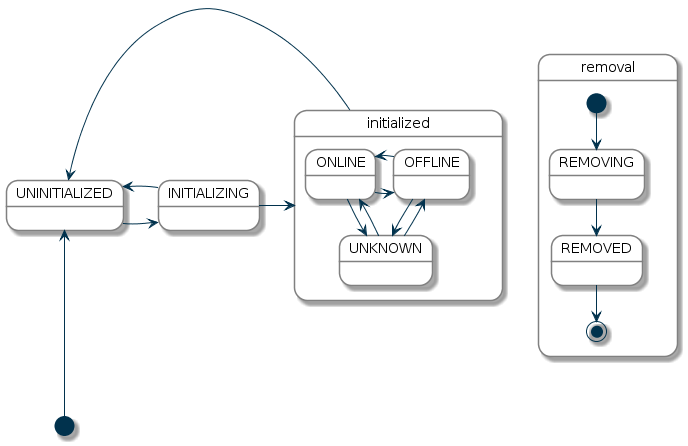
\includegraphics[width=12cm]{Immagini/status_transitions}
    \caption{Transizioni di Stato}
    \label{fig:status_transitions}
\end{figure}

Gli stati UNINITIALIZED, INITIALIZED, REMOVING e REMOVED sono impostati dal framework mentre UNKNOWN, ONLINE e OFFLINE sono assegnati dal binding. Sono rappresentate le transizioni tra i vari stati alla Figura \ref{fig:status_transitions}.

\subsection{Channels} Vengono forniti dalle {\em things} e rappresentano le diverse loro funzioni. Dove la {\em thing} è un'entità fisica o la fonte di informazione, il {\em channel} è una funzione concreta di questa. Una lampadina fisica({\em thing}) potrebbe avere un canale della temperatura del colore({\em channel 1}) e un canale del colore({channel 2}), che forniscono entrambi la funzionalità dell'unica {\em thing} della lampadina al sistema. Per le fonti di informazione, la {\em thing} potrebbe essere il tempo locale con informazioni da un servizio web con diversi {\em channels} come temperatura, pressione e umidità. I {\em channels} sono collegati agli {\em items} e questi collegamenti sono il collante tra livello fisico e virtuale. Stabilito il collegamento una {\em thing} reagisce agli eventi inviati per un {\em item} collegato ad uno dei suoi {\em channels} e a sua volta una {\em thing} può inviare eventi attraverso gli {\em item} sfruttando uno dei suoi {\em channel}.

\subsection{Items} {\em OpenHAB} applica una forte separazione tra mondo fisico ({\em Things}) e mondo virtuale ({\em Items}). Gli {\em Items} rappresentano in particolarità le funzionalità usate dall'applicazione. Essi hanno uno {\em stato} e vengono usati attraverso degli {\em eventi}. Gli {\em Items} disponibili sono rappresentati alla Tabella \ref{tab:items}.

\begin{table}[]
    \centering
    \begin{tabular}{l|p{5cm}|p{5cm}}
        \textbf{Nome Item} & \textbf{Descrizione} & \textbf{Tipo di Comando} \\
        \hline
        Color & Informazione sul colore(RGB) & OnOff, IncreaseDecrease, Percent, HSB\\
        Contact & Stato di memorizzazione dell'articolo & OpenClosed\\
        DateTime & Memorizzazione data e ora & -\\
        Dimmer & Valore percentuale del dimmer & OnOff, IncreaseDecrease, Percent\\
        Group & Oggetto che ne raccoglie altri & -\\
        Image & Contiene i dati binari dell'immagine & -\\
        Location & Memorizza le coordinate GPS & Point\\
        Number & Memorizza valori nel formato numero e può avere una dimensione opzionale per il suffizzo & Decimal\\
        Number:\textless dimension\textgreater & Come Number ma con un'informazione addizionale per l'unità supportata & Quantity\\
        Player & Permette di controllare i players come i riproduttori musicali & PlayPause, NextPrevious, RewindFastforward\\
        Rollershutter & Tipicamente utilizzati per le tapparelle & UpDown, StopMove, Percent\\
        String & Memorizza testi & String\\
        Switch & Usati tipicamente per le luci & OnOff
    \end{tabular}
    \caption{Items}
    \label{tab:items}
\end{table}

Gli {\em items} \textbf{group} possono contenere {\em items} o {\em groups} al loro interno. In questo modo a livello di interfaccia utente viene vista una sola voce per il {\em group} che poi può fornire in dettaglio la vista di ogni singolo membro. Il raggruppamento ciclico non è vietato ma fortemente sconsigliato. Un esempio rappresentante la configurazione di un gruppo è alla Figura \ref{fig:group_item_example}.

\begin{figure}
    \centering
    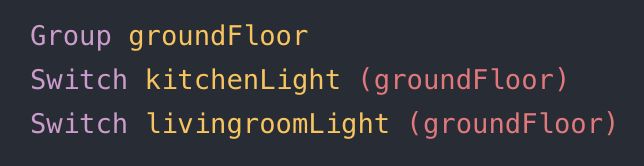
\includegraphics{Immagini/GroupItemExample}
    \caption{Esempio Group Item}
    \label{fig:group_item_example}
\end{figure}

{\em Group items} possono derivare il proprio stato dai loro membri; per fare ciò i {\em group} devono essere costruiti a partire da un {\em base item} e una {\em group function}. Nel calcolare lo stato la {\em group function} attraversa i membri di gruppi e sottogruppi e se trova un {\em item} che definisce lui stesso uno stato allora viene preso questo come stato del gruppo.

Il {\em formato} dei vari {\em items sarà}
\begin{itemize}
    \item \textbf{StringType}: normali java strings
    \item \textbf{DateTimeType}: java SimpleDateFormat.parse() usando come matching pattern yyyy-MM-dd'T'HH:mm:ss.SSSZ, yyyy-MM-dd'T'HH:mm:ss.SSSz, yyyy-MM-dd'T'HH:mm:ss.SSSX, yyyy-MM-dd'T'HH:mm:ssz, yyyy-MM-dd'T'HH:mm:ss
    \item \textbf{DecimalType, PercentType}: java BigDecimal e java PercentType con valori tra 0 e 100
    \item \textbf{QuantityType}: valore numerico più un unità numerica
    \item \textbf{HSBType}: tre valori numerici separati dalla virgola che corrispondono a {\em Hue} (tonalità) compreso tra 0 e 360, {\em Saturation} (saturazione) compresa tra 0 e 100 e {\em Brightness} (luminosità) compresa tra 0 e 100
    \item \textbf{PointType}: sono tre valori numerici separati dalla virgola che indicano {\em latitudine}, {\em longitudine} e {\em altitudine}. I primi due vengono rappresentati in gradi mentre il terzo in metri.
    \item  \textbf{EnumTypes}: rappresentati alla Tabella \ref{tab:enum_types}
\end{itemize}

\begin{table}[]
    \centering
    \begin{tabular}{l|l}
        \textbf{Type} & \textbf{Valore supportato} \\
        \hline
        IncreaseDecreaseType & INCREASE, DECREASE\\
        NextPreviousType & NEXT, PREVIOUS\\
        OnOffType & ON, OFF\\
        OpenClosedType & OPEN, CLOSED\\
        PlayPauseType & PLAY, PAUSE\\
        RewindFastforwardType & REWIND, FASTFORWARD\\
        StopMoveType & STOP, MOVE\\
        UpDownType & UP, DOWN
    \end{tabular}
    \caption{EnumTypes}
    \label{tab:enum_types}
\end{table}

A volte è necessario allegare informazioni aggiuntive agli elementi per determinati casi d'uso. Potrebbe trattarsi di un'applicazione che necessita di alcuni suggerimenti per rendere gli {\em items} in modo generico, o un'integrazione con assistenti vocali, o qualsiasi altro servizio che accede agli {\em items} e ha bisogno di comprenderne il significato. Per questo ci sono gli {\em items metadata} che possono essere allegati agli {\em item} utilizzando namespaces. Ogni metadata è una entry che ha un valore principale o una coppia opzionale di chiave/valore (esempio: Switch MyFan "My Fan" {homekit="Fan.v2", alexa="Fan" [type="oscillating", speedSteps=3]}).

\subsection{Rules} Servono per automatizzare dei processi. Ogni regola invoca uno script che esegue dei tasks. Le {\em rules} sono nella cartella \textbf{\$OPENHAB\_CONF/rules}. Vi sono degli esempi dai quali partire nel demo file chamato {\em demo.rules}. Un file può contenere diverse regole che condividono lo stesso contesto di esecuzione. Le regole possono essere manipolate anche da UI. Ciò è possibile tramite l'accesso al web server tramite browser e andando nella sezione Settings/Rules. Quì tramite l'icona + è possibile aggiungere una nuova regola inserendo un {\em nome} e impostando un {\em trigger}. In seguito bisogna aggiungere un'azione che verrà scaturita dell'attivazione del trigger. Questa è lo script che andremo ad aggiungere. \'E possibile inserire o un ECMAScript in javascript o un Rule DSL in un linguaggio proprietario di openHAB. L'estensione {\em openHAB VS Code Extension} aiuta il programmatore a scrivere in modo corretto le {\em rules} per Rule DSL.

Il {\em rule file} è strutturato in 
\begin{itemize}
    \item Imports
    \item Variable Declarations
    \item Rules
\end{itemize}

\paragraph{Imports} sono come in java; infatti non fanno altro che importare delle librerie per usarle all'interno del file. Esempio al Codice \ref{code:rules_import}.

\begin{lstlisting}[caption=Import, label=code:rules_import]
import java.net.URI
\end{lstlisting}

\paragraph{Variable Declarations} sono variabili usate dalle {\em rules} del file. Esse possono avere o no un valore iniziale e possono essere modificabili o read-only. Esempio al Codice \ref{code:rules_variable_declarations}.

\begin{lstlisting}[caption=Variable Declarations, label=code:rules_variable_declarations]
// a variable with an initial value. Note that the variable type is automatically inferred
var counter = 0

// a read-only value, again the type is automatically inferred
val msg = "This is a message"

// an uninitialized variable where we have to provide the type (as it cannot be inferred from an initial value)
var Number x
\end{lstlisting}

\paragraph{Rules} contengono la lista di regole e la loro sintassi deve essere come quella dell'esempio al Codice \ref{code:rules_rules}

\begin{lstlisting}[caption=Rules,label=code:rules_rules]
rule "<RULE_NAME>"
when
    <TRIGGER_CONDITION> [or <TRIGGER_CONDITION2> [or ...]]
then
    <SCRIPT_BLOCK>
end
\end{lstlisting}

\begin{itemize}
    \item \textless RULE\_NAME\textgreater: ogni regola deve avere un nome univoco e possibilmente con un significato associato
    \item \textless TRIGGER\_CONDITION\textgreater: sono le condizioni tramite le quali vengono applicate le regole. Una regola viene eseguita quando si verifica la sua condizione. Possono essere aggiunte più condizioni separate dalla parola chiave {\em or}
    \item \textless SCRIPT\_BLOCK\textgreater: corrisponde alla logica che viene eseguita quando una certa condizione diventa vera
\end{itemize}

\subsubsection{Triggers}
Vi sono differenti tipi di {\em trigger} che possono essere inseriti
\begin{itemize}
    \item \textbf{Item}(-Event)-based triggers: reagiscono agli eventi sul bus degli eventi openHAB, ovvero reagiscono a comandi o aggiornamenti di stato degli {\em Items}
    \item \textbf{Member of}(-Event)-based triggers: reagiscono agli eventi sul bus degli eventi openHAB per gli {\em Items} che fanno parte del gruppo fornito
    \item \textbf{Time}-based triggers: reagiscono ad una certa ora preimpostata
    \item \textbf{System}-based triggers: reagiscono ad un certo stato del sistema
    \item \textbf{Thing}-based triggers: reagiscono ad uno stato di una {\em thing}, per esempio il cambio tra online e offline
\end{itemize}

\paragraph{Event-based Triggers}: \'E possibile ascoltare i comandi per un {\em item} specifico, sugli aggiornamenti di stato. Può essere scelto se catturare solo un comando/stato specifico o uno qualsiasi. La sintassi per questi casi è al Codice \ref{code:event-based_triggers}.

\begin{lstlisting}[caption=Event-based Triggers,label=code:event-based_triggers]
Item <item> received command [<command>]
Item <item> received update [<state>]
Item <item> changed [from <state>] [to <state>]
\end{lstlisting}

\paragraph{Member of Triggers}: come event-based triggers ma dei membri di un gruppo dato. Le variabili implicite vengono popolate dall'{\em item} che causa l'evento. La variabile {\em triggerItem} viene popolata dalll'{\em item} che ha causato il trigger della {\em rule}. Esempio al Codice \ref{code:member_of_triggers}. I {\em member of triggers} lavorano con i membri diretti di un gruppo e non con gruppi nidificati.

\begin{lstlisting}[caption=Member of Triggers,label=code:member_of_triggers]
Member of <group> received command [<command>]
Member of <group> received update [<state>]
Member of <group> changed [from <state>] [to <state>]
\end{lstlisting}

\paragraph{Time-based Triggers}: si possono usare espressioni predefinite per le ore o espressioni cronologiche. I campi di un'espressione cronologica possono essere 6 o 7:
\begin{enumerate}
    \item Seconds
    \item Minutes
    \item Hours
    \item Day-of-Month
    \item Month
    \item Day-of-week
    \item Year (opzionale)
\end{enumerate}
Un esempio è al Codice \ref{code:time-based_triggers}.

\begin{lstlisting}[caption=Time-based Triggers,label=code:time-based_triggers]
Time is midnight
Time is noon
Time cron "<cron expression>"
\end{lstlisting}

\paragraph{System-based Triggers}: si dovrebbe usare System started trigger per inizializzare i valori allo startup se non lo sono. Esempio al Codice \ref{code:system-based_triggers}.

\begin{lstlisting}[caption=System-based Triggers,label=code:system-based_triggers]
rule "Speedtest init"
when
    System started
then
    createTimer(now.plusSeconds(30), [|
        if (Speedtest_Summary.state == NULL || Speedtest_Summary.state == "") Speedtest_Summary.postUpdate("unknown")
    ])
end
\end{lstlisting}

\paragraph{Thing-based Triggers}: si possono catturare eventi di cambiamento o aggiornamento di uno stato generato da una particolare {\em thing}. Si possono catturare uno specifico aggiornamento/cambiamento di stato o qualsiasi. La sintassi è mostrata con un esempio al Codice \ref{code:thing-based_triggers}.

\begin{lstlisting}[caption=Thing-based Triggers,label=code:thing-based_triggers]
Thing <thingUID> received update [<status>]
Thing <thingUID> changed [from <status>] [to <status>]
\end{lstlisting}

\paragraph{Channel-based Triggers} alcuni add-ons forniscono dei {\em trigger channels}. Un {\em trigger channel} fornisce informazioni su eventi discreti e non continui. Si può reagire ad uno specifico o ad ogni trigger che il {\em channel} fornisce. Vi è l'esempio al Codice \ref{code:channel-based_triggers}.

\begin{lstlisting}[caption=Channel-based Triggers,label=code:channel-based_triggers]
Channel "<triggerChannel>" triggered [<triggerEvent>]
\end{lstlisting}

\subsubsection{Scripts}

Il linguaggio delle espressioni usato negli {\em scripts} è lo stesso usato nel linguaggio Xtend. La sintassi è simile a java ma ci sono molte caratteristiche che permettono di scrivere il codice in modo più coinciso (come nell'uso delle collections). Non c'è bisogno che gli {\em scripts} vengano compilati ma possono essere interpretati. OpenHAB fornisce accesso a 
\begin{itemize}
    \item tutti gli {\em items} definiti, accessibili dal proprio nome
    \item tutti gli {\em stati/comandi} enumerati (ON, OFF, DOWN, ...)
    \item tutte le {\em standard actions}
\end{itemize}
Tramite la combinazione di questi possono essere creati {\em scripts} come l'esempio al Codice \ref{code:script_example}

\begin{lstlisting}[caption=Esempio Script,label=code:script_example]
if (Temperature.state < 20) {
    Heating.sendCommand(ON)
}
\end{lstlisting}

Le {\em Rules} vengono usate per manipolare lo stato o il valore di un {\em item}. Due comandi possono essere
\begin{itemize}
    \item MyItem.postUpdate(\textless new\_state\textgreater) - cambia lo stato di un {\em item} senza causare azioni implicite.
    \item MyItem.sendCommand(\textless new\_state\textgreater ) - cambia lo stato di un {\em item} e scatena i trigger di potenziali altre azioni.
\end{itemize}

Spesso nelle {\em rules} è necessario manipolare lo stato di un {\em item}. Ogni {\em item} in openHAB ha uno stato accessibile tramite l'attributo {\em state} (esempio: MyItem.state). Per usare uno stato di un {\em item} è necessario conoscere il {\em tipo} di stato e come convertire questo in valori di tipi primitivi con i quali possono essere fatte operazioni. Vengono divisi i tipi di comando e i tipi di stato. Per semplicità è possibile aggiungere la parola ``{\em type"} alla fine del comando per capire il tipo di stato come all'esempio al Codice \ref{code:example_state_type}.

\begin{lstlisting}[caption=Esempio State Type,label=code:example_state_type]
MyColorItem.sendCommand(ON) // --> OnOffType
MyColorItem.sendCommand(INCREASE) // --> IncreaseDecreaseType
MyColorItem.sendCommand(new PercentType(50)) // --> PercentType
MyColorItem.sendCommand(new HSBType(new DecimalType(123), new PercentType(45), new PercentType(67))) // --> HSBType
\end{lstlisting}

I {\em group} possono essere dichiarati con qualsiasi {\em item type} e lo stato interno del gruppo sarà di quel tipo (esempio: Group:Switch sarà OnOffType). Ciascun tipo di stato fornisce dei metodi utili per conversioni e calcoli. Variabili predefinite sono disponibili e possono essere utilizzate nelle regole. Esse sono 
\begin{itemize}
    \item \textbf{receivedCommand} - implicitamente disponibile in ogni regola che ha almeno un command event trigger
    \item \textbf{previousState} - implicitamente disponibile in ogni regola che ha almeno uno status change event trigger
    \item \textbf{newState} - implicitamente disponibile in ogni regola che ha almeno uno status update o status change event trigger
    \item \textbf{triggeringItemName} - implicitamente disponibile in ogni regola che ha almeno uno status update, uno status change o un command event trigger
    \item \textbf{triggeringItem} - implicitamente disponibile in ogni regola che ha un ``Member of" trigger
    \item \textbf{receivedEvent} - implicitamente disponibile in ogni regola che ha un channel-based trigger
\end{itemize}

\subsection{Sitemap}
In openHAB {\em things} e {\em items} rappresentano gli oggetti fisici e logici della domotica dell'utente. Le {\em sitemap} vengono utilizzate per selezionare e preparare questi elementi al fine di comporre una presentazione orientata all'utente di questa configurazione per varie interfacce utente.

Le {\em sitemaps} sono file di testo con estensione .sitemap e vengono archiviate nella cartella \textbf{\$OPENHAB\_CONF/sitemaps}. Vi è di default un file demo denominato {\em demo.sitemap} da cui partire per configurarla in base alle proprie esigenze. Vi è un esempio del codice al Codice \ref{code:sitemap_code_example} e quello che viene prodotto dal codice alla Figura \ref{fig:sitemap_view_example}.

\begin{lstlisting}[caption=Esempio Codice di una Sitemap,label=code:sitemap_code_example]
sitemap demo label="My home automation" {
    Frame label="Date" {
        Text item=Date
    }
    Frame label="Demo" {
        Switch item=Lights icon="light"
        Text item=LR_Temperature label="Livingroom [%.1f °C]"
        Group item=Heating
        Text item=LR_Multimedia_Summary label="Multimedia [%s]" icon="video" {
            Selection item=LR_TV_Channel mappings=[0="off", 1="DasErste", 2="BBC One", 3="Cartoon Network"]
            Slider item=LR_TV_Volume
        }
    }
}
\end{lstlisting}

\begin{figure}
    \centering
    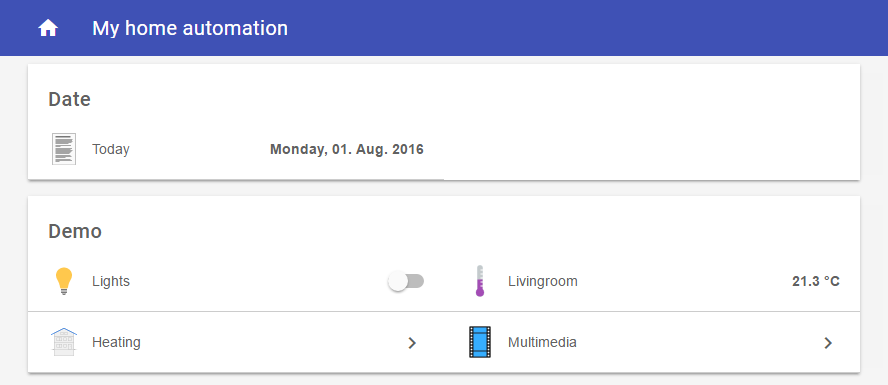
\includegraphics[width=12cm]{Immagini/SitemapViewExample}
    \caption{Esempio di View di una Sitemap}
    \label{fig:sitemap_view_example}
\end{figure}

\paragraph{Elements} le {\em sitemaps} sono composte da vari elementi. L'esempio contiene come elementi {\em Frame}, {\em Text} e {\em Switch}. Gli elementi presentano informazioni, consentono l'interazione e sono altamente configurabili in base allo stato del sistema. Una riga di definizione dell'elemento della {\em sitemap} produce un elemento dell'interfaccia utente corrispondente. Come mostrato nell'esempio, ogni elemento genera un testo descrittivo accanto a un'icona sul lato sinistro e uno stato e/o elementi di interazione sulla destra.

\paragraph{Parameters} è possibile configurare un determinato set di parametri per personalizzare la presentazione di un elemento. Nell'esempio mostrato {\em item} e {\em label} sono parametri. Quasi tutti i parametri sono opzionali, alcuni sono tuttavia necessari per ottenere un'interfaccia utente significativa. Per evitare righe di definizione degli elementi molto lunghe o non strutturate, i parametri possono essere suddivisi in più righe di codice.

\paragraph{Blocks} incapsulando gli elementi con parentesi graffe, è possibile annidare più elementi all'interno di altri. Il tipo di elemento {\em Frame} viene spesso utilizzato in combinazione con i blocchi di elementi. I frame vengono utilizzati per distinguere visivamente più elementi dello stesso argomento su una pagina dell'interfaccia. Quando si utilizzano blocchi di codice con altri tipi di elementi come {\em Text} o {\em Group}, questi elementi dell'interfaccia utente, oltre alla loro normale funzione, saranno collegamenti a una nuova vista, presentando gli elementi nidificati. Nell'esempio precedente, sono definiti più {\em Frame} e alcuni elementi non sono visibili nella vista principale ma sono accessibili dietro il loro elemento genitore. Questi sono indicati dall'icona di controllo ``\textgreater" a destra di un elemento.

\paragraph{Dependencies} una tipica {\em sitemap} contiene dozzine di singoli elementi. Lo stato del sistema e le possibili interazioni sono tuttavia spesso strettamente dipendenti. OpenHAB supporta queste dipendenze fornendo parametri per il comportamento dinamico.

L'elemento {\em sitemap} è obbligatorio nella definizione di una {\em sitemap}. Nell'esempio del Codice \ref{code:sitemap_code_example} alla riga 1 troviamo l'elemento {\em sitemap} con
\begin{itemize}
    \item {\em sitemapname} ovvero {\em demo}. Deve essere lo stesso nome del file, quindi il file contenete tale codice deve chiamarsi {\em demo.sitemap}.
    \item {\em label} ovvero {\em My home automation}. Esso è il testo della {\em sitemap} mostrato a video.
\end{itemize}

Gli elementi che possono essere utilizzati in una {\em sitemap} possono essere quelli della Tabella \ref{tab:sitemap_element_types}.

\begin{table}[]
    \centering
    \begin{tabular}{l|p{10cm}}
        \textbf{Element} & \textbf{Descrizione} \\
        \hline
        Chart & Aggiunge un oggetto grafico rappresentante una serie temporale per i dati persistiti\\
        Colorpicker & Permette l'utente di scegliere un colore da una color wheel\\
        Default & Esegue il rendering di un elemento nella rappresentazione dell'interfaccia utente predefinita specificata dal tipo di elemento specificato\\
        Frame & Stabilisce un'area contenente vari altri elementi della sitemap\\
        Group & Concentra tutti gli elementi di un dato gruppo in un blocco annidato\\
        Image & Rende un'immagine data da un URL\\
        Mapview & Visualizza una mappa OSM basata su un determinato elemento posizione\\
        Selection & Fornisce un menu a discesa o un popup modale che presenta i valori tra cui scegliere per un elemento\\
        Setpoint & Rende un valore compreso tra i pulsanti di aumento e diminuzione\\
        Slider & Presenta un valore in un cursore simile a una barra di avanzamento\\
        Switch & Rende un oggetto come interruttore ON/OFF o multi-pulsante\\
        Text & Rende un oggetto come testo\\
        Video & Visualizza un flusso video, dato un URL\\
        Webview & Visualizza il contenuto di una pagina web
    \end{tabular}
    \caption{Tipi di Elementi di una Sitemap}
    \label{tab:sitemap_element_types}
\end{table}

\section{Modello Semantico}
Uno degli scopi di openHAB è quello di astrarre gli smart device vedendoli nel modo più generico possibile così da mantenere una logica semplice e facilmante gestibile con l'annessione di qualsiasi altro dispositivo. Proprio per questo vengono usati gli {\em items} che nascondono l'oggetto fisico. Essi sono le entità principali con le quali lavorano le API Rest di openHAB. I vari {\em items} vengono raccolti in un modello semantico che permette di organizzarli in maniera semplice ed intuitiva in modo tale da semplificare l'uso da parte dell'utente.

\begin{figure}
    \centering
    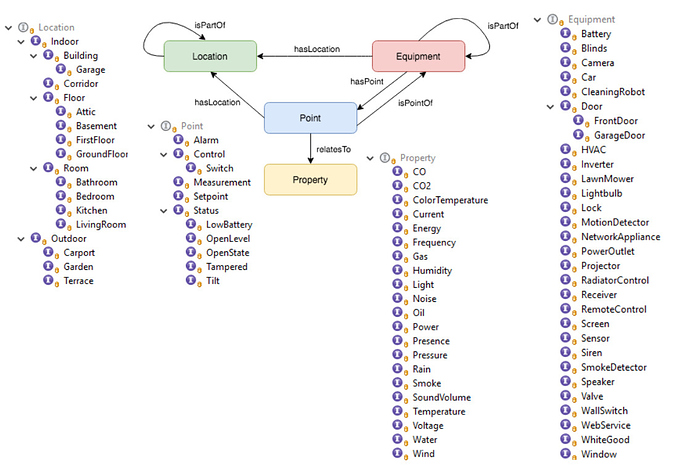
\includegraphics[width=12cm]{Immagini/ontology_relationships}
    \caption{Relazioni Ontologiche}
    \label{fig:ontology_relationships}
\end{figure}

Come rappresentato all'esempio della Figura \ref{fig:ontology_relationships} vi sono 4 concetti fondamentali nel modello semantico
\begin{itemize}
    \item \textbf{Location} è un {\em group item} che può contenere altre location, equipments e points e rappresenta una posizione fisica (edificio, stanza, ...). Una Location può essere membro di un solo Location Group
    \item \textbf{Equipment} è normalmente un {\em group item} che può contenere un equipment secondario e points. Un Equipment può essere membro diretto di una sola Location o un solo Equipment
    \item \textbf{Point} non è un gruppo, ma rappresenta qualsiasi altro tipo di elemento ed è solitamente collegato a un channel. Un Point può essere membro diretto di una sola Location o un solo Equipment
    \item \textbf{Property} è un tag aggiuntivo su un point item che indica che tipo di punto è (esempio: un termometro potrebbe essere un point di tipo misurazione con una property di tipo temperatura)
\end{itemize}

A Figura \ref{fig:example_model} vi è un esempio avanzato di modello.
\begin{figure}
    \centering
    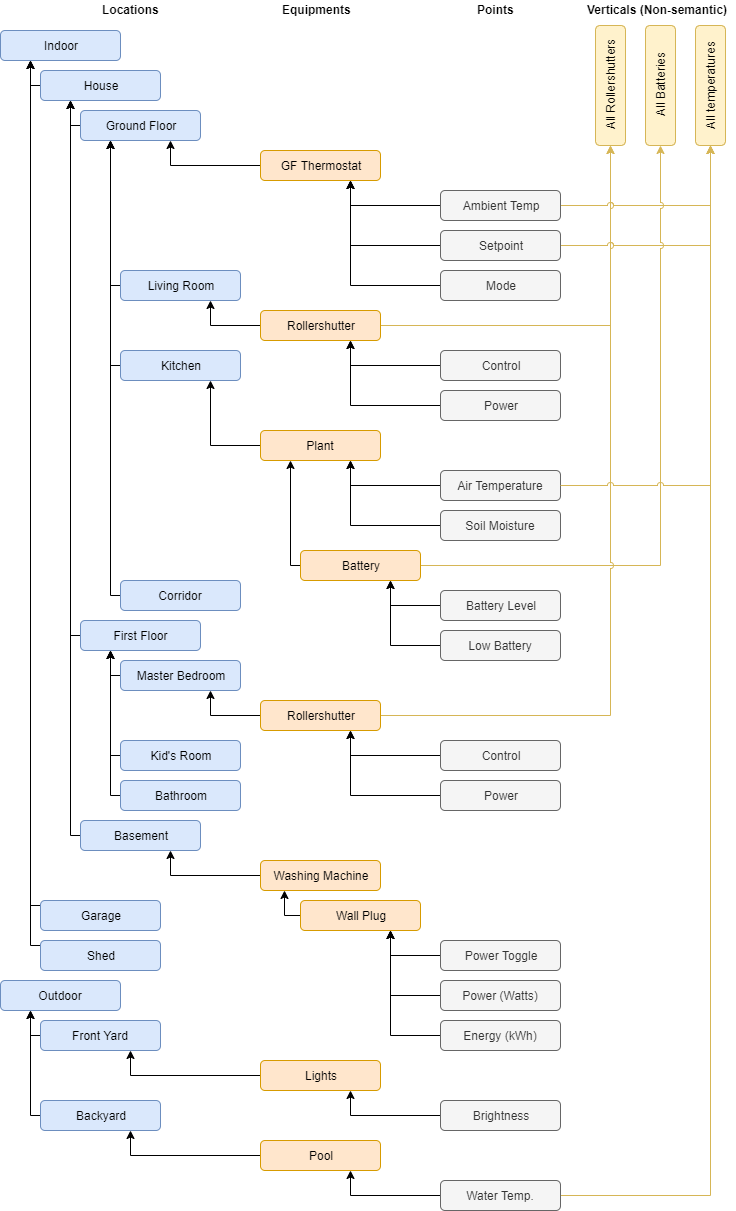
\includegraphics[width=12cm]{Immagini/example_model}
    \caption{Esempio di Modello}
    \label{fig:example_model}
\end{figure}

\section{Persistence}
OpenHAB permette di tenere traccia degli stati storici degli {\em items} attraverso l'uso della persistenza. Con essa quindi si può 
\begin{itemize}
    \item Tracciare un grafico della lettura di un sensore di temperatura nel tempo
    \item Ripristinare un elemento allo stato che aveva prima della chiusura o del riavvio di openHAB
    \item Usare lo stato di un oggetto nel passato, o qualche aggregato dello stato di un oggetto nel passato (esempio: Media da un'ora fa) nelle regole di automazione 
\end{itemize}

Per persistere i dati vengono forniti più database sia interni che esterni. Quelli esterni richiedono l'installazione e la configurazione su server separato.

Quando {\em persistence} salva gli stati degli {\em items}?
\begin{itemize}
    \item quando un {\em item} cambia
    \item quando un {\em item} viene aggiornato
    \item quando un {\em item} riceve un comando
    \item ogni minuto se ha ricevuto un evento
\end{itemize}

Una strategia di persistenza è {\em restoreOnStartup} che permette di aggiornare gli {\em items} con gli stati salvati più recentemente. Può essere possibile creare nella cartella  \\\textbf{\$OH\_CONF/persistence} un file con estensione {\em .persist} per definire la strategia di persistenza. 

Il database predefinito per la persistenza è \texttt{rrdj4} e viene fornito con strategie {\em everyChange}, {\em everyMinute} e {\em restoreOnStartup}. La comodità di questo database è che rimane sempre di una dimensione preimpostata e non c'è bisogno di pulirlo. Per eseguire tale logica rimpiazza i vecchi records con quelli nuovi. Questo approccio non funziona con tutti i tipi di {\em items}.

\section{openHAB REST API}
Tramite le REST API di openHAB è possibile accedere alla piattaforma da altre applicazioni e manipolare i dati visti nella struttura. Ciò include l'accesso ad {\em Item}, {\em Things} e {\em Bindings} e la modificazione dei vari stati. Le interazioni con l'API REST si basano su protocollo {\em http}. \'E possibile accedere tramite {\em internet} all'API REST ma a discapito della sicurezza, poiché in tale modo si espone openHAB a chiunque è in rete. Gli utenti infatti sono incoraggati a garantire connessioni sicure e protette. {\em OpenHAB API REST} può non essere installata automaticamente ma una volta fatto è accessibile tramite la dashboard.

Esempi di applicazioni di REST API in openHAB sono
\begin{itemize}
    \item Recupera i dati openHAB da applicazioni esterne
    \item Inietta dati e attiva eventi in openHAB da applicazioni esterne (esempio: alcuni rilevatori di movimento o telecamere di sorveglianza)
    \item Ispeziona bindings, things o items di openHAB, scopri gli states, i parametri o i problemi correnti
    \item Interagire con openHAB da altri programmi; molti linguaggi di programmazione e strumenti di automazione possono facilmente utilizzare l'API REST
    \item Utilizzo di software di terze parti sui telefoni cellulari, come tasker per aprire la porta del garage
\end{itemize}

Esempi di applicazione pratica tramite il tool {\em curl} che permette di fare chiamate REST al servizio server
\begin{itemize}
    \item Commutazione My\_ItemOFF mediante l'emissione di un HTTP POST richiesta
    \begin{lstlisting}
    curl -X POST --header "Content-Type: text/plain" --header "Accept: application/json" -d "OFF" "http://{openHAB_IP}:8080/rest/items/My_Item"
    \end{lstlisting}
    \item Impostare una voce di contatto My\_Item su CHIUSO emettendo una richiesta http PUT a My\_Item/state
    \begin{lstlisting}
    curl -X PUT --header "Content-Type: text/plain" --header "Accept: application/json" -d "CLOSED" "http://{openHAB_IP}:8080/rest/items/My_Item/state"
    \end{lstlisting}
    \item Recupero di un elenco di tutti gli items e groups mediante l'emissione di una richiesta GET
    \begin{lstlisting}
    curl -X GET --header "Accept: application/json" "http://{openHAB_IP}:8080/rest/items?recursive=false"
    \end{lstlisting}
    \item Recupero di un elenco di tutte le sitemap mediante l'emissione di una richiesta GET
    \begin{lstlisting}
    curl -X GET --header "Accept: application/json" "http://{openHAB_IP}:8080/rest/sitemaps"
    \end{lstlisting}
    \item Iscrizione agli eventi
    \begin{lstlisting}
    curl "http://{openHAB_IP}:8080/rest/events?topics=smarthome/things/{thingUID}/statuschanged"
    curl "http://{openHAB_IP}:8080/rest/events?topics=smarthome/channels/{channelUID}/triggered"
    \end{lstlisting}
\end{itemize}

OpenHAB supporta anche la protezione tramite password per contenuti sensibili come parti del modello semantico. I meccanismi forniti per tale scopo sono l'{\em basic authentication} e l'{\em OAuth authorization}. La maggior parte dei linguaggi di programmazione già supporta queste tecnologie. Per aggiungere utente e password nelle chiamate {\em curl} basta aggiungere \texttt{-u \{USER\_NAME\}} e poi inserire la password richiesta. Per fare tutto con un singolo comando basta aggiungere \texttt{-u \{USER\_NAME:PASSWORD\}}. Con l'API token basta aggiungere il comando \texttt{-u \{API\_TOKEN\}}.

\'E possibile creare un API Token dal proprio profilo accedendo con username da amministratore e password, andando sul profilo e premendo su \texttt{Create new API token}. Illustrazione a Figura \ref{fig:apitoken_login}.

\begin{figure}
    \centering
    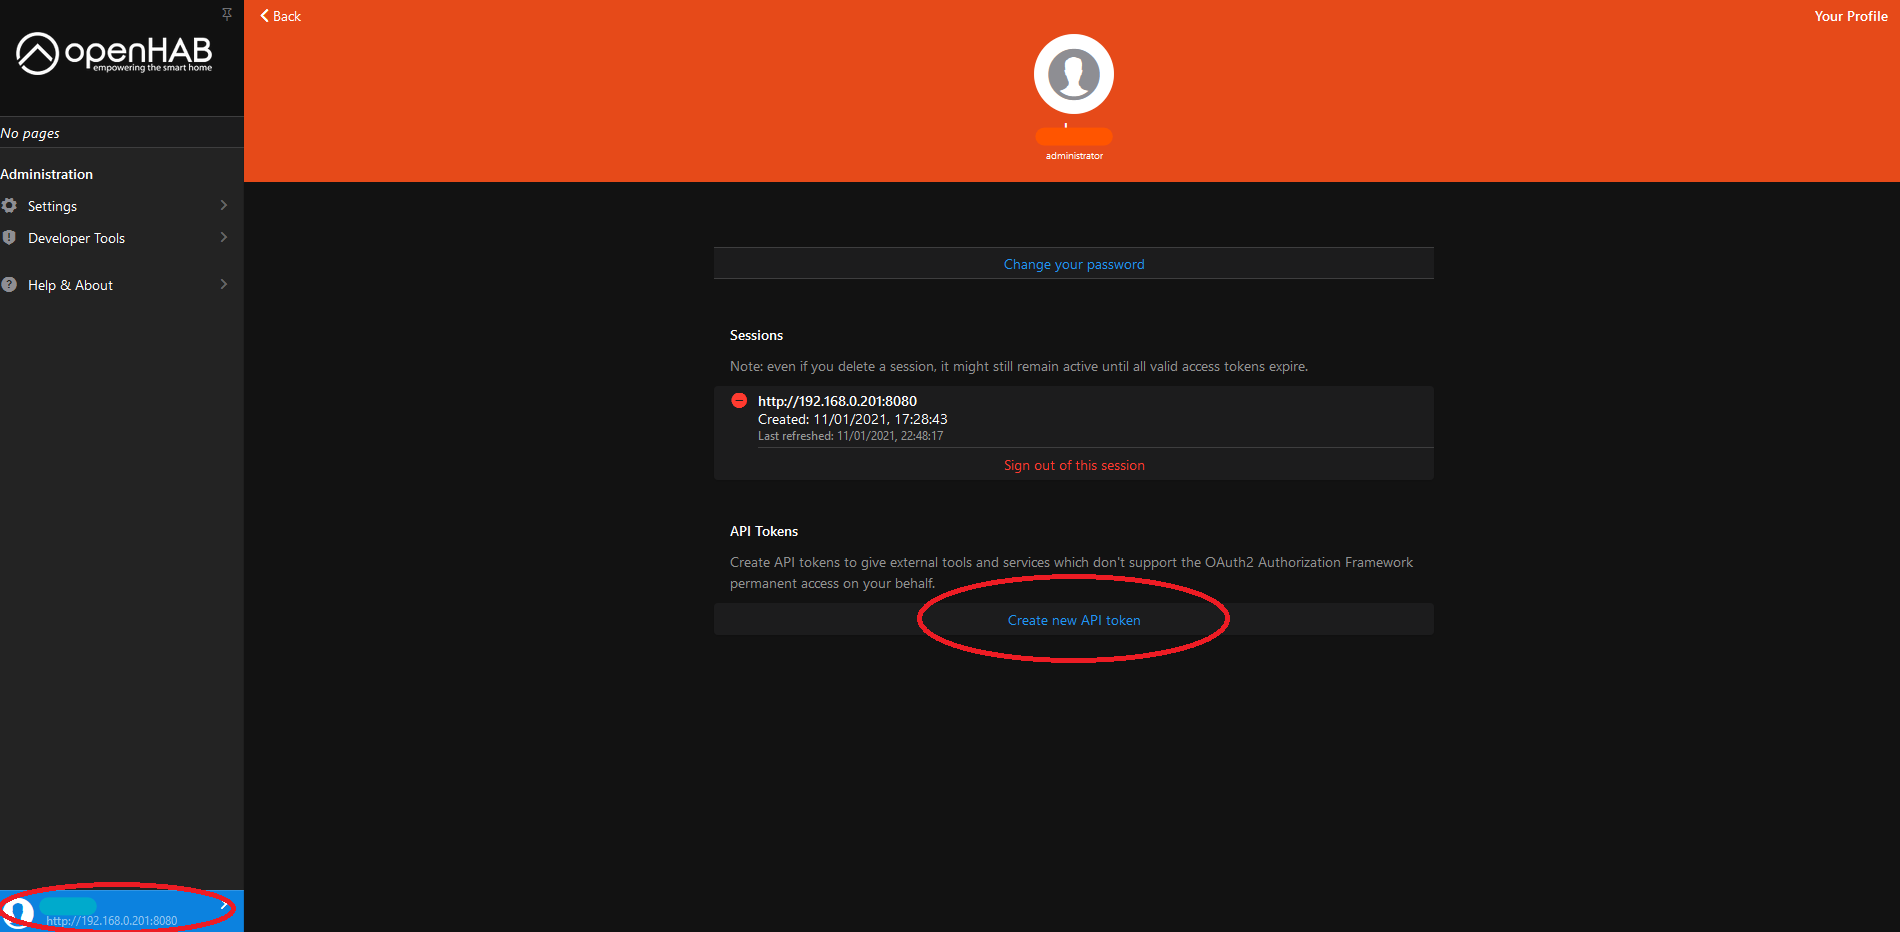
\includegraphics[width=14cm]{Immagini/apitoken_login}
    \caption{API Token Login}
    \label{fig:apitoken_login}
\end{figure}
\chapter{MQTT Binding}
\begin{figure}
    \centering
    
\includegraphics{Immagini/mqtt_logo.png}
    \caption{MQTT Logo}
    \label{fig:mqtt_logo}
\end{figure}

Come già spiegato alla sezione \ref{chap:binding_intro} un {\em binding} permette di connettere un dispositivo fisico ad una {\em thing}. In questo caso specifico \'e stato sviluppato un {\em sistema IOT} per sperimentare l'associazione con openHAB. Per collegare il device ed il framework \'e stato utilizzato il protocollo di rete \textbf{MQTT}.

\section{Protocollo MQTT}
{\em Message Queuing Telemetry Transport} \'e un protocollo di rete leggero di tipo {\em  publish-subscribe} che funziona su TCP/IP. MQTT \'e progettato per connessioni con postazioni remote in cui è richiesta un'impronta di codice ridotta o una larghezza di banda della rete limitata \cite{enwiki:1023769301}.

Il protocollo definisce due tipi di entit\'a di rete:
\begin{itemize}
    \item \textbf{broker}
    \item \textbf{client}
\end{itemize}
Esse vengono illustrate a Figura \ref{fig:mqtt_model_structure}.

\begin{figure}
    \centering
    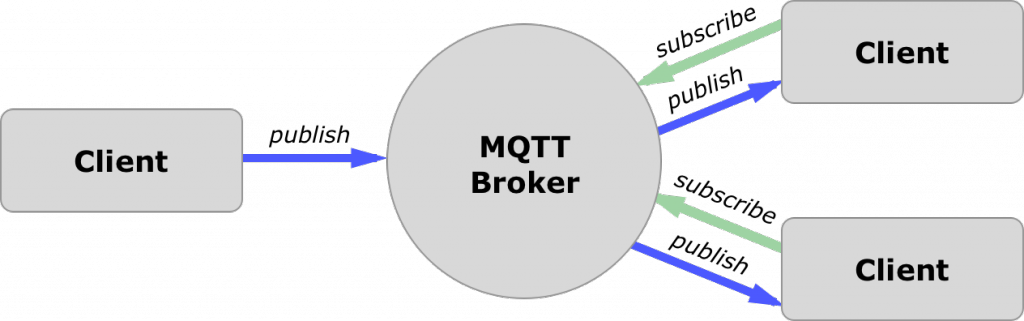
\includegraphics[width=12cm]{Immagini/mqtt_model_structure.png}
    \caption{MQTT Model Structure}
    \label{fig:mqtt_model_structure}
\end{figure}

\paragraph{broker} server che riceve tutti i messaggi dai {\em client} e li instrada ai {\em client} di destinazione appropriati. Il {\em broker MQTT} \'e un software in esecuzione su un computer in locale o remoto. Di esso sono disponibili sia implementazioni open source che proprietarie. Il {\em broker} riceve solitamente messaggi da un {\em publisher} che distribuisce a pi\'u {\em subscriber}. Sia il {\em publisher} che il {\em subscriber} sono {\em client MQTT}. Il {\em broker} mantiene traccia di tutte le informazioni della sessione mentre i dispositivi si accendono e si spengono. Esse vengono chiamate {\em persistent sessions}.

\paragraph{client} qualsiasi dispositivo che esegue una libreria MQTT per connettersi ad un broker MQTT in rete. Un {\em client} ha dialogo diretto solamente con un broker e non con altri {\em client}; il broker infatti fa da tramite tra lui e gli altri. I {\em client} possono {\em pubblicare} o {\em sottoscriversi} per inviare o riceve dati.

\paragraph{topic} le informazioni sono organizzate in gerarchie di argomenti chiamati {\em topic}. Quando un {\em client} vuole inviare un messaggio ad un altro, basta che lo invia al broker con lo stesso {\em topic} a cui \'e sottoscritto il {\em client}. 

\paragraph{retained message} Se viene inviato un messaggio al {\em broker} relativo ad un {\em topic} dove non vi sono {\em client} sottoscritti viene scartato. Ci\'o non viene fatto nel caso di {\em retained message}. Esso \'e un normale messaggio MQTT con flag {\em retain} a true. In caso viene inviato un {\em retained message}, questo viene memorizzato insieme al rispettivo QoS. In tal caso quindi possono essere salvati gli ultimi messaggi nei propri {\em topic} cos\'i da notificare un subscriber degli ultimi dati inviati appena si sottoscrive.

\paragraph{message types} sono utizzati durante la connessione illustrata a Figura \ref{fig:mqtt_connection}.
\begin{itemize}
    \item \textbf{connect}: aspetta una connessione con il {\em broker} e crea un collegamento tra i nodi
    \item \textbf{disconnect}: attende la terminazione del lavoro da parte del {\em client} e la disconnessione della sessione TCP/IP.
    \item \textbf{publish}: ritorna il messaggio inviato da un {\em client MQTT} al broker immediatamente al thread dell'applicazione di ogni client sottoscritto allo stesso topic.
\end{itemize}

\begin{figure}
    \centering
    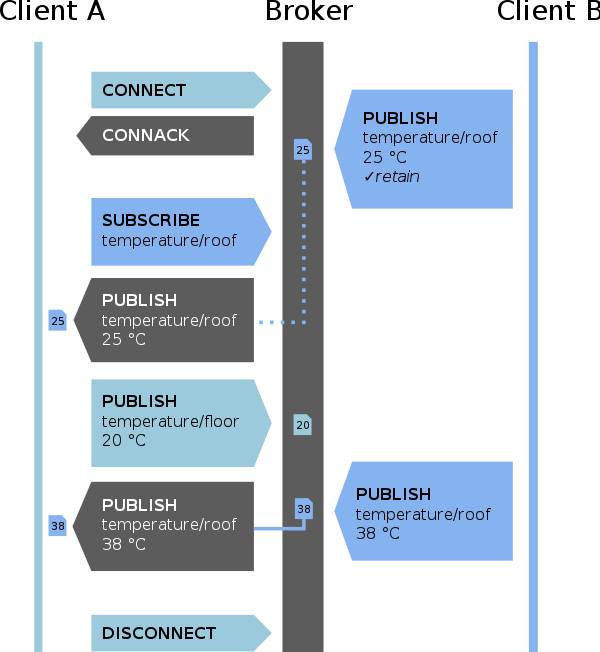
\includegraphics[width=12cm]{Immagini/mqtt_connection.png}
    \caption{MQTT Connection}
    \label{fig:mqtt_connection}
\end{figure}

\section{openHAB Binding}
{\em openHAB} implementa un {\em binding} gi\'a configurato per il protocollo MQTT. Tale protocollo ha un'architettura client/server. Il server di MQTT, ovvero il {\em broker} NON viene fornito nel binding di openHAB ma pu\'o essere utilizzato qualsiasi altro software che f\'a da {\em broker MQTT} come {\em Mosquitto}. Il {\em binding openHAB} permette di configurare le connessioni ai broker tramite le {\em openHAB things}. L'associazione non permette per\'o di collegare i {\em channels} ai {\em topic} o di eseguire il rilevamento automaticodei {\em topic} disponibili. I {\em bridge} supportati sono: 

\begin{itemize}
    \item \textbf{Broker}: {\em bridge} che rappresenta una connessione {\em broker MQTT} configurata e gestita da tale {\em binding}.
    \item \textbf{SystemBroker}: un {\em broker} configurato dal sistema non pu\'o essere modificato da questo {\em binding} e verr\'a elencato come {\em broker} di sistema di sola lettura.
\end{itemize}

\subsection{Configurazione bridge}
\begin{itemize}
    \item \textbf{host}: IP/hostname del broker MQTT. {\em Binding} che consente una connessione univoca con {\em host:porta}.
    \item \textbf{port}: se non ne viene fornita nessuna vengono utilizzate quelle di default che sono 1883 e 8883(SSL). {\em Binding} che consente una connessione univoca con {\em host:porta}.
    \item \textbf{secure}: se si vuole utilizzare una connessione sicura con il {\em broker} tramite TLS/SSL. Pu\'o essere true o false. Di default \'e false.
\end{itemize}

Altri parametri da impostare possono essere:
\begin{itemize}
    \item \textbf{qos}: indica qualit\'a del servizio che pu\'o essere imposrtata a 0, 1 o 2 (default 0).
    \item \textbf{clientID}: ID client fisso che viene generato automaticamente.
\end{itemize}

I parametri di riconnessione sono:
\begin{itemize}
    \item \textbf{reconnectTime}: tempo di riconnessione in millisecondi. Valore del tempo di attesa aspettato per una connessione dopo che ne viene persa una. Il valore predefinito \'e 60000 (60s).
    \item \textbf{keepAlive}: tempo in secondi utile per capire se una connessione al server \'e persa o no. IL valore di default \' 60s.
\end{itemize}

Pu\'o essere impostato un LWT(testamento) MQTT:
\begin{itemize}
    \item \textbf{lwtMessage}: messaggio del testamento. Default vuoto.
    \item \textbf{lwtTopic}: topic del testamento. Default vuoto.
    \item \textbf{lwt}: qos del testamento. Default 0.
    \item \textbf{lwtRetain}: conserva l'ultimo messaggio. True o false, false di default.
\end{itemize}

Inoltre si possono impostare i seguenti parametri opzionali:
\begin{itemize}
    \item \textbf{username}: nome utente MQTT
    \item \textbf{password}: password MQTT
    \item \textbf{certificatepin}: se impostato dopo che \'e stata stabilita una connessione controlla il certificato. Se questo risulta non essere valido viene interrotta la connessione. Questa opzione aumenta la sicurezza.
    \item \textbf{publickeypin}: se impostata dopo che \'e stata stabilita una connessione controlla la chiave pubblica. Se questa risulta non essere valida viene interrotta la connessione. Questa opzione aumenta la sicurezza.
    \item \textbf{certificate}: hash del certificato utile per verificarne l'autenticit\'a per mezzo di {\em certificatepin}.
    \item \textbf{publickey}: hash della chiave pubblica utile per verificarne l'autenticit\'a per mezzo di {\em publickeypin}.
    \item \textbf{enableDiscovery}: di default sono abilitati i servizi di rilevamento sul broker. Questi possono essere controllati per mezzo di tale parametro.
\end{itemize}

\subsection{Things supportate}
Data la struttura molto generica di MQTT, il {\em binding}  consente di aggiungere un numero arbitrario di {\em thinngs MQTT} generiche. Su ogni {\em thing} possono essere aggiunti un numero arbitrario di {\em channels}.

\subsubsection{Channels supportati}
\begin{itemize}
    \item \textbf{string}: invia o riceve del testo su un {\em topic MQTT}.
    \item \textbf{number}: invia o riceve un numero su un {\em topic MQTT}.
    \item \textbf{dimmer}: gestisce un valore percentuale.
    \item \textbf{contact}: rappresenta uno stato di OPEN/CLOSE.
    \item \textbf{switch}: invia o riceve uno stato ON/OFF su un {\em topic MQTT}.
    \item \textbf{color}: gestisce i valori di un colore nei formati HSB, RGB o xyY (x, y, luminosit\'a)..
    \item \textbf{location}: gestisce una posizione.
    \item \textbf{image}: gestisce un'immagine binaria nei formati supportati da Java (bmp, jpg, png).
    \item \textbf{datetime}: gestisce un valore data/ora.
    \item \textbf{rollershutter}: gestisce una tapparella.
\end{itemize}

\subsection{Configurazione channel}
\begin{itemize}
    \item \textbf{stateTopic}: {\em topic MQTT} che rappresenta lo stato della {\em thing}. Possono essere utilizzati caratteri jolly per recuperare lo stato da pi\'u {\em topic}.
    \item \textbf{trasformationPattern}: pattern di trasformazione opzionale applicato a tutti i valori di entrata.
    \item \textbf{trasformationPatternOut}: pattern di trasformazione opzionale applicato a tutti i valori di uscita.
    \item \textbf{commandTopic}: {\em topic} per inviare comandi in uscita. Se non viene impostato il {\em channel} \'e in modalit\'a read-only.
    \item \textbf{formatBeforPublish}: utile per formattare un valore prima che viene pubblicato nel {\em broker MQTT}. Di default \'e utilizzato per il passaggio tra {\em channel} e {\em item}.
    \item \textbf{postCommand}: azione che permette di inviare ad altri elementi il valore ricevuto per un particolare {\em topic MQTT}.
    \item \textbf{retained}: verr\'a inviato il valore come messaggio MQTT mantenuto.
    \item \textbf{qos}: qos del {\em channel}.
    \item \textbf{trigger}: se true il {\em topic} dello stato aggiorner\'a un {\em channel} al suo posto.
\end{itemize}

\subsubsection{string}
\begin{itemize}
    \item \textbf{allowStates}: elenco separato da virgole di stati consentiti.
\end{itemize}


\subsubsection{number}
\begin{itemize}
    \item \textbf{min}: valore minimo
    \item \textbf{max}: valore massimo
    \item \textbf{step}: per canali aumenta o decrementa
    \item \textbf{unit}: unit\'a di misura
\end{itemize}

\subsubsection{contact, switch}
\begin{itemize}
    \item \textbf{on}: un numero opzionale (come 1, 10) o una stringa (come ``ON''/``Open'') riconosciuti come stato on/open.
    \item \textbf{off}: un numero opzionale (come 0, -10) o una stringa (come ``OFF''/``Close'') riconosciuti come stato off/close.
\end{itemize}

\subsubsection{color}
\begin{itemize}
    \item \textbf{color\_mode}: stringa obbligatoria che defisnisce la rappresentazione del colore: ``hsb'', ``rgb'', ``xyY''.
    \item \textbf{on}: una stringa facoltativa (come ``BRIGHT'') riconoscita come on.
    \item \textbf{off}: una stringa facoltativa (come ``DARK'') riconoscita come off.
    \item \textbf{onBrightness}: se collegato ad un {\em item} switch ed \'e acceso.
\end{itemize}

\subsubsection{location}
Pu\'o essere collegato tale {\em channel} ad un {\em Location item}. Esso pubblicher\'a la posizione come elenco separato da virgole sul broker MQTT (esempio: ``112,54,123'', ovvero latitudine, longitudine e altitudine).

\subsubsection{image}
Pu\'o essere collegato tale {\em channel} ad un {\em Image item} ed \'e di tipo read-only. I valori devono essere in binario e del formato supportato da java (bmp, jpg, png).

\subsubsection{datetime}
Pu\'o essere collegato tale {\em channel} ad un {\em DateTime item}. Pubblicher\'a la data/ora nel formato ``aaaa-MM-gg'T'HH::mm''.

\subsubsection{rollershutter}
\begin{itemize}
    \item \textbf{on}: stringa facoltativa come ``Open'' riconosciuta come UP.
    \item \textbf{off}: stringa facoltativa come ``Close'' riconosciuta come DOWN.
    \item \textbf{stop}: stringa facoltativa come ``Stop'' riconosciuta come STOP.
\end{itemize}

\subsection{Rule actions}
Tale {\em binding} include una regola di azione che consente di pubblicare messaggi MQTT dall\'interno. delle regole.

\begin{lstlisting}[caption=Esempio Rule Action Istanza,label=code:rule_action_example_instance]
val mqttActions = getActions("mqtt","mqtt:systemBroker:embedded-mqtt-broker")
\end{lstlisting}

Nel Codice \ref{code:rule_action_example_instance} il primo parametro deve essere sempre \texttt{mqtt} mentre il secondo \'e il Thing UID del broker usato. Una volta recuparata l'stanza d'azione basta pubblicare con in comando \texttt{publishMQTT(String topic, String value, Boolean retain)} come nel Codice \ref{code:rule_action_example_publish}.

\begin{lstlisting}[caption=Esempio Rule Action Pubblicazione,label=code:rule_action_example_publish]
mqttActions.publishMQTT("mytopic","myvalue", true)
\end{lstlisting}
\chapter{Configurazione dell'MQTT Binding per un sistema IOT}
Per testare openHAB con un sistema IOT si \'e deciso di procedere allo sviluppo di uno {\em Smart Garden}, ovvero un sistema per la gestione automatizzata del proprio giardino. Di base si tratta di un sensore per la misurazione dell'umidit\'a del terreno e una pompa per l'attivazione dell'innaffiamento in caso di siccit\'a.

\section{Smart Garden}
Il sistema IOT quindi nello specifico \'e composto da:
\begin{itemize}
    \item \textbf{Soil Moisture Sensor}: sensore di umidit\'a del terreno (Figura \ref{fig:soil_moisture_sensore}).
    \item \textbf{Water Pump}: pompa dell'acqua utile per irrigare alla sua attivazione (Figura \ref{fig:water_pump}).
    \item \textbf{Raspberry Pi}: unit\'a logica che permette di rendere dinamica l'interazione tra i sensori. \'E la centralina del sistema IOT (Figura \ref{fig:raspberry_pi}).
    \item \textbf{Rel\'e}: elemento utile per l'attivazione e disattivazione della pompa (Figura \ref{fig:rele}).
    \item \textbf{Alimentatore da 12 Volt}: alimentazione della pompa (Figura \ref{fig:12v_power_supply}).
\end{itemize}

\subsubsection{Soil Moisture Sensore}
\begin{figure}
    \centering
    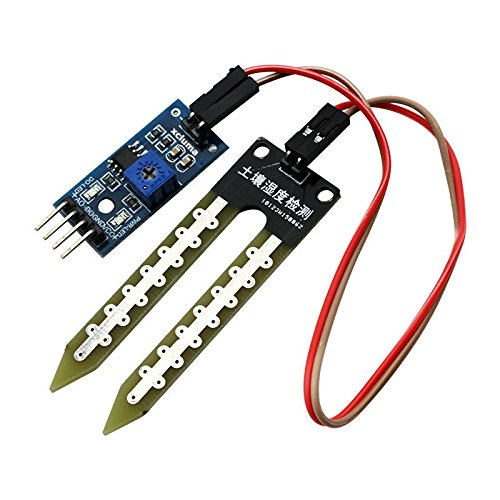
\includegraphics[width=8cm]{Immagini/soil_moisture_sensore}
    \caption{Soil Moisture Sensore}
    \label{fig:soil_moisture_sensore}
\end{figure}
Il {\em Soil Moisture Sensor} \'e un sensore che rileva l'umidit\'a del suolo. Esso ha una forma a ferro di cavallo dove alle due estremit\'a vi sono due contatti. Tra i contatti del sensore viene fatta passare una tensione, tanto maggiore è l'umidit\'a tra i due contatti, tanto minore sar\'a la resistenza, permettendo alla corrente di fluire da un contatto verso l'altro. 

Esso ha lo scopo di segnalare o meno la presenza di umidit\'a cos\'i da scatenare poi l'evento di start o stop della pompa dell'acqua. Il sensore viene collegato per mezzo di cavi ai pin della Raspberry Pi per inviare segnali di input.

\subsubsection{Water Pump}
\begin{figure}
    \centering
    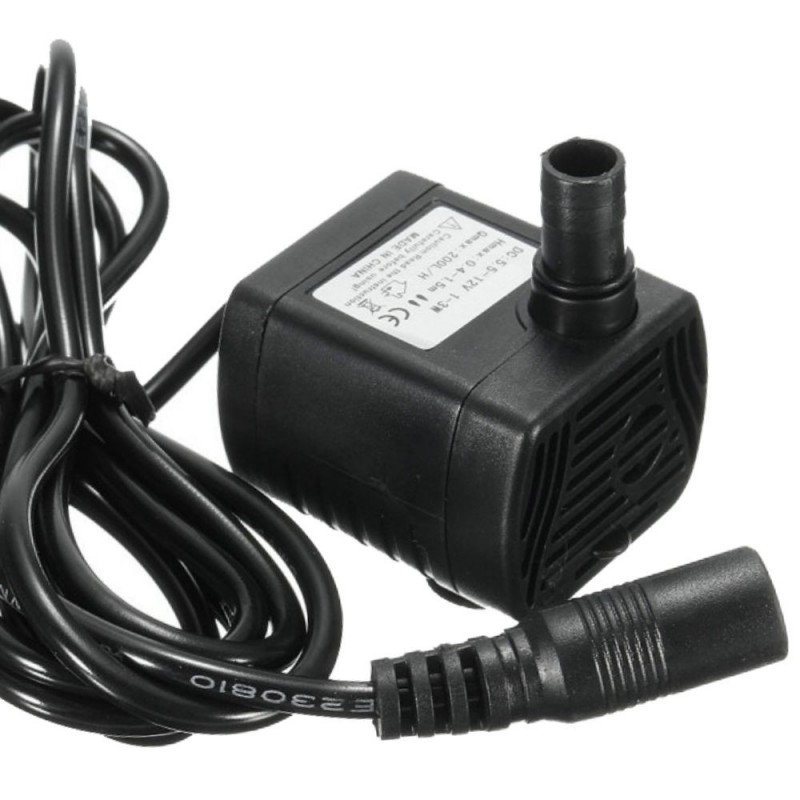
\includegraphics[width=8cm]{Immagini/water_pump}
    \caption{Water Pump}
    \label{fig:water_pump}
\end{figure}
La Pompe dell'Acqua permette di prendere l'acqua e dirigerla verso una direzione per l'irrigazione del proprio giardino. Essa ha la caratteristica di essere totalmente immersa nell'acqua e presenta nella parte superiore un buco nella quale viene infilato un tubo che sar\'a poi collegato nell'altra estremit\'a ad un erogatore d'acqua utile ad innaffiare.

La Pompa viene collegata tramite cavi ad un Rel\'e per la sua attivazione ed all'alimentatore da 12 volt poiché la raspberry non pu\'o sostenere tale carico. Essa viene attivata in caso di siccit\'a e spenta altrimenti.

\subsubsection{Raspberry Pi}
\begin{figure}
    \centering
    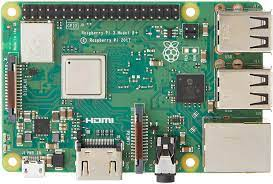
\includegraphics[width=8cm]{Immagini/raspberry_pi}
    \caption{Raspberry Pi}
    \label{fig:raspberry_pi}
\end{figure}
Centralina del sistema IOT. Essa permette di essere programmata per leggere e controllare i vari dispositivi che gli vengono collegati. Per collegarsi ad un sessore o dispositivo esterno vengono messsi a disposizione dei pin ai quali vengono agganciati dei cavi.

La Raspberry viene collegata ai vari sensori e dispositivi per implementare la logica del sistema.

La Raspberry Pi \'e dotata di una scheda di rete tramite la quale comunicher\'a esternamente con il device in cui \'e installato openHAB.

\subsubsection{Rel\'e}
\begin{figure}
    \centering
    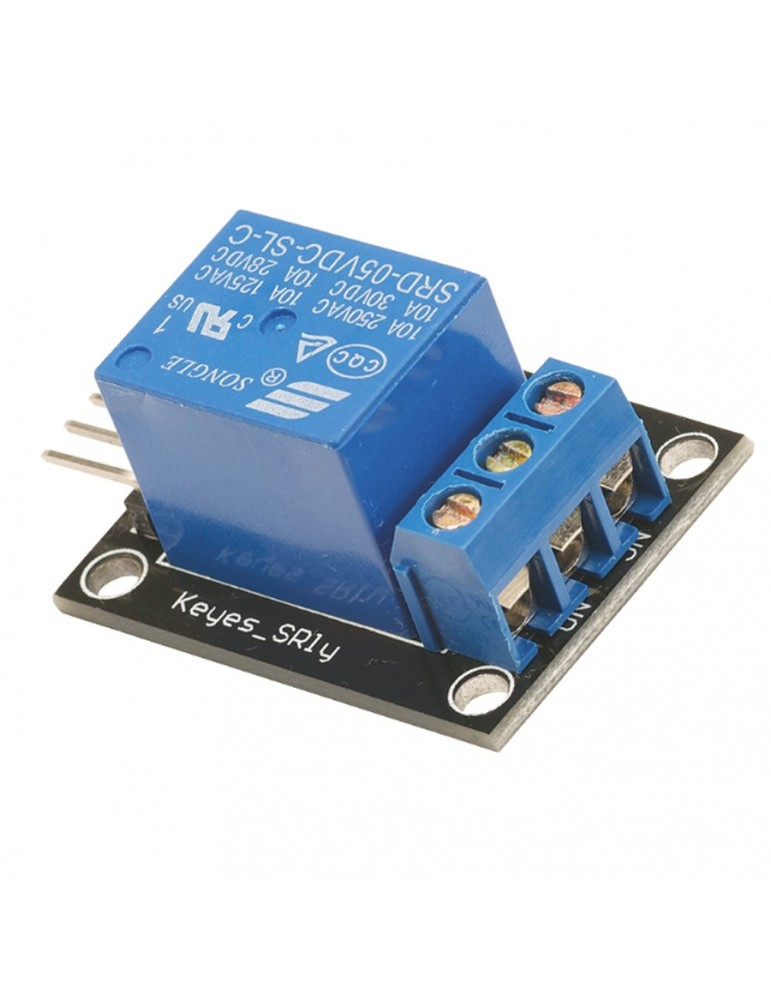
\includegraphics[width=8cm]{Immagini/rele}
    \caption{Rel\'e}
    \label{fig:rele}
\end{figure}
Elemento che permette tramite il passaggio della corrente di attivarsi o disattivarsi. Esso \'e come un pulsante che si accende e si spegne al passaggio della corrente.

Utile nel sistema per attivare e disattivare la Pompa. La Raspberry quando vuole attivare/disattivare la Water Pump attiva/disattiva il Rel\'e che a sua volta attiva/disattiva il circuito tra Pompa e la sua alimentazione.

\subsubsection{Alimentatore da 12 Volt}
\begin{figure}
    \centering
    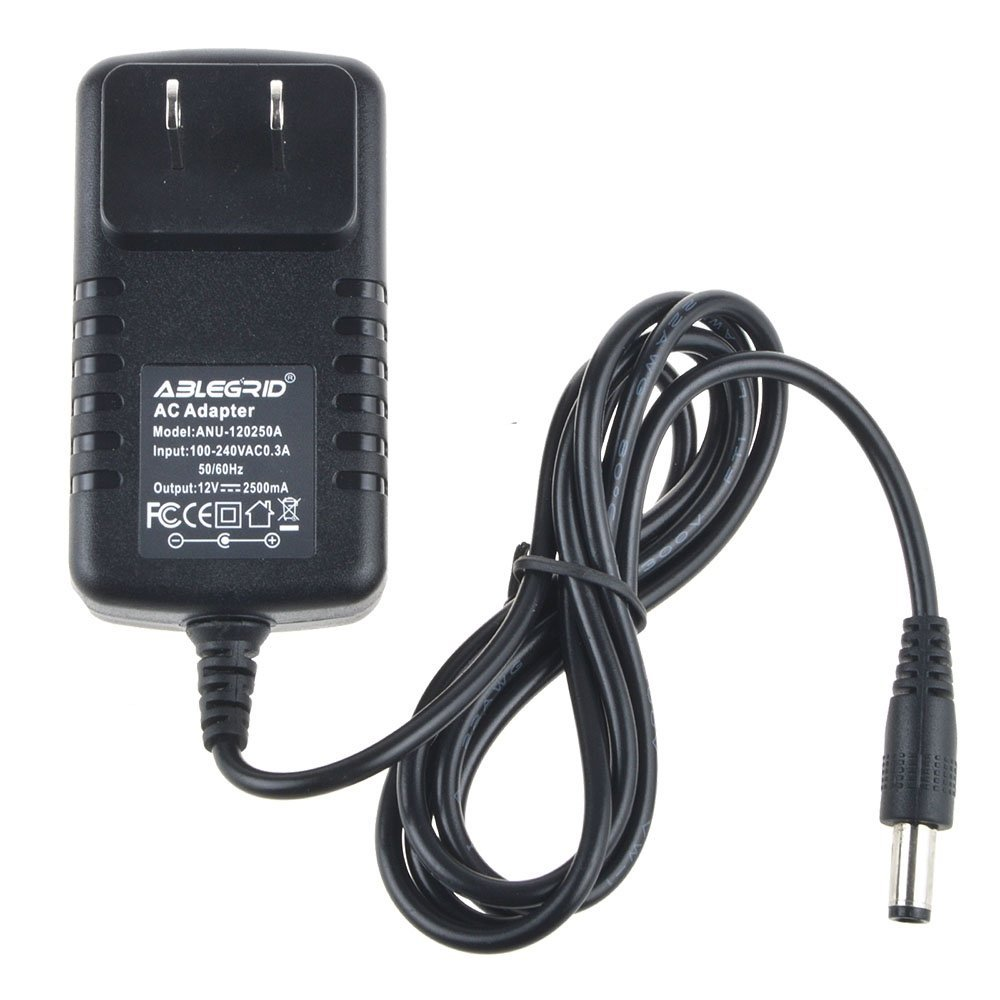
\includegraphics[width=8cm]{Immagini/12v_power_supply}
    \caption{Alimentatore da 12 Volt}
    \label{fig:12v_power_supply}
\end{figure}
Alimentazione utile per attivare la pompa. Essa non poteva funzionare con l'alimentazione fornita da Raspberry che arriva massimo a 5 volt. 

L'alimentatore viene collegato al Rel\'e e alla pompa.

\'E possibile visualizzare un semplice schema dei collegamenti a Figura \ref{fig:smart_garden_structure}.

\begin{figure}
    \centering
    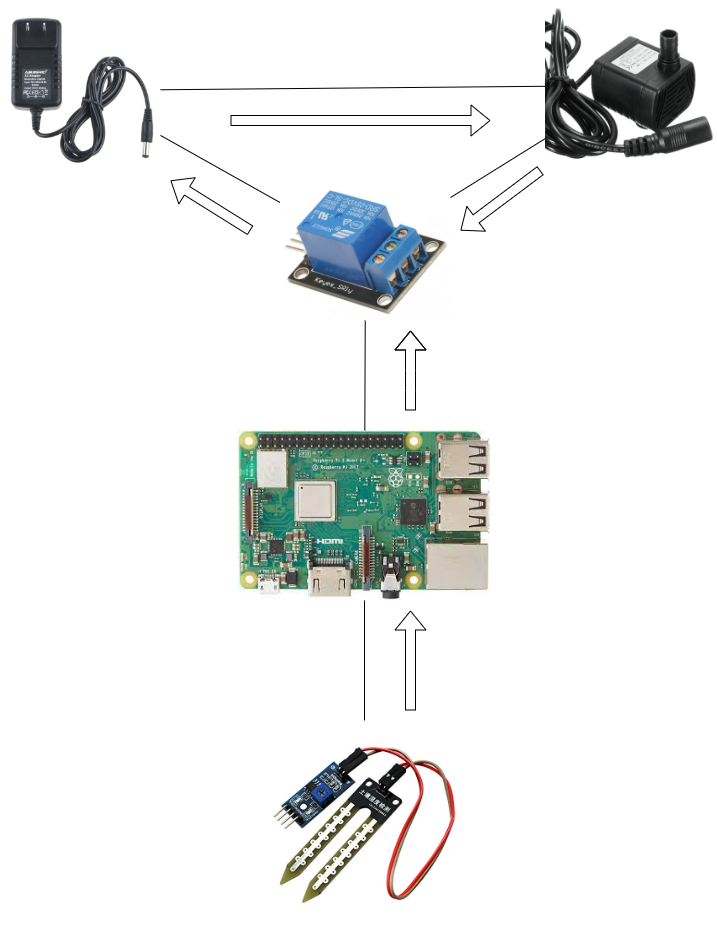
\includegraphics[width=12cm]{Immagini/smart_garden_structure}
    \caption{Struttura Smart Garden}
    \label{fig:smart_garden_structure}
\end{figure}

\subsection{Sviluppo sistema IOT}
Il sistema IOT viene controllato tramite Raspberry Pi da un piccolo programma python. Esso ha accesso tramite la libreria \texttt{RPi.GPIO} ai pin per gestire i dispositivi o sensori agganciati. Il programma legge in input il valore prelevato dal sensore di umidit\'a mentre attiva e disattiva in output la pompa tramite il rel\'e. Tutto ci\'o viene gestito tramite protocollo MQTT con libreria \texttt{paho.mqtt.client}. Tramite dei topic infatti si pu\'o:
\begin{itemize}
    \item leggere il sensore di umidit\'a
    \item attivare o disattivare la pompa manualmente
    \item attivare o disattivare il sistema in modalit\'a automatica, ovvero sar\'a lui ad attivare o disattivare la pompa in caso non ci sia o ci sia un terreno umido.
\end{itemize}

\subsubsection{Codice del sistema IOT}
Il programma \'e composto da 4 file principali.
\begin{itemize}
    \item \textbf{Soil.py}: contiene la classe per la creazione dell'oggetto capace di gestire il sensore di umidit\'a del terreno.
    \item \textbf{Pump.py}: contiene la classe per la creazione dell'oggetto capace di gestire il rel\'e per controllare la pompa dell'acqua.
    \item \textbf{MQTTClient.py}: contiene la classe per la creazione dell'oggetto capace di fare publish e subscribe in MQTT.
    \item \textbf{main.py}: file main da cui ha inizio il programma ed in cui \'e la logica di business.
\end{itemize}

\begin{lstlisting}[caption=Soil.py, label=code:soil.py]
import RPi.GPIO as GPIO

class Soil:

    def __init__(self, channel):
        self.channel = channel
        GPIO.setmode(GPIO.BCM)
        GPIO.setup(self.channel, GPIO.IN)

    def status(self):
        return GPIO.input(self.channel)
\end{lstlisting}

\begin{lstlisting}[caption=Pump.py, label=code:pump.py]
import RPi.GPIO as GPIO

class Pump:

    def __init__(self, channel):
        self.channel = channel
        GPIO.setmode(GPIO.BCM)
        GPIO.setup(self.channel, GPIO.OUT)

    def on(self):
        GPIO.output(self.channel, GPIO.HIGH)

    def off(self):
        GPIO.output(self.channel, GPIO.LOW)
\end{lstlisting}

\begin{lstlisting}[caption=MQTTClient.py, label=code:mqtt_client.py]
import paho.mqtt.client as mqtt

class MQTTClient:

    def __init__(self, ip, port):
        self.ip = ip
        self.port = port

    def publish(self, topic, to_publish):
        self.client = mqtt.Client()
        self.client.connect(self.ip, self.port, 60)
        self.client.publish(topic, to_publish, 0, True);
        self.client.disconnect()

    def subscribe(self, topic, on_message):
        client = mqtt.Client()
        client.connect(self.ip, self.port, 60)
        client.on_connect = lambda client, userdata, flags, rc : self.on_connect(client, userdata, flags, rc, topic)
        client.on_message = on_message
        client.loop_start()
        return client

    def on_connect(self, client, userdata, flags, rc, topic):
        print("[" + topic + "]: connected with result code " + str(rc))
        client.subscribe(topic)
\end{lstlisting}

\begin{lstlisting}[caption=main.py, label=code:main.py]
import time
import threading

from MQTTClient import MQTTClient
from Soil import Soil
from Pump import Pump

import os
from os.path import join, dirname
from dotenv import load_dotenv

dotenv_path = join(dirname(__file__), '.env')
load_dotenv(dotenv_path)

# mqtt connection data
MQTT_IP = os.environ.get("MQTT_IP")
MQTT_PORT = (int)(os.environ.get("MQTT_PORT"))

# topics
TOPIC_HANDLE_PUMP = os.environ.get("TOPIC_HANDLE_PUMP")
TOPIC_HANDLE_AUTO = os.environ.get("TOPIC_HANDLE_AUTO")
TOPIC_STATUS_SOIL = os.environ.get("TOPIC_STATUS_SOIL")

# pins
PIN_PUMP = (int)(os.environ.get("PIN_PUMP"))
PIN_SOIL = (int)(os.environ.get("PIN_SOIL"))

# global variable to start and stop auto
stop_thread = True

mqtt_client = MQTTClient(MQTT_IP, MQTT_PORT)

soil = Soil(PIN_SOIL)
pump = Pump(PIN_PUMP)

# threading functions
def publish_pump(status):
    global status_thread
    if not stop_thread:
        mqtt_client.publish(TOPIC_HANDLE_PUMP, status)

def callback():
    if soil.status():
        publish_pump('ON')
        mqtt_client.publish(TOPIC_STATUS_SOIL, 'Water Not Detected')
    else:
        publish_pump('OFF')
        mqtt_client.publish(TOPIC_STATUS_SOIL, 'Water Detected')

def loop():
    while True:
        callback()
        time.sleep(1)

# on_message functions
def on_message_auto(client, userdata, msg):
    global stop_thread
    stop_thread = msg.payload.decode() != "ON"

def on_message_pump(client, userdata, msg):
    global pump
    if msg.payload.decode() == "ON":
        pump.on()
    else:
        pump.off()

# main function
if __name__ == "__main__":
    thread = threading.Thread(target=loop)
    thread.start()
    mqtt_client.subscribe(TOPIC_HANDLE_AUTO, on_message_auto)
    mqtt_client.subscribe(TOPIC_HANDLE_PUMP, on_message_pump)
\end{lstlisting}

In breve alla partenza del programma vengono inizializzate le costanti prelevate dalle variabili d'ambiente relative a 
\begin{itemize}
    \item \textbf{MQTT\_IP}: IP del client MQTT.
    \item \textbf{MQTT\_PORT}: porta del client MQTT.
    \item \textbf{TOPIC\_HANDLER\_PUMP}: topic MQTT per gestire l'attivazione e la disattivazione manuale della pompa.
    \item \textbf{TOPIC\_HANDLER\_AUTO}: topic MQTT per gestire l'attivazione e la disattivazione della modalit\'a automatica.
    \item \textbf{TOPIC\_STATUS\_SOIL}: topic MQTT per leggere lo stato del sensore di umidit\'a del suolo.
    \item \textbf{PIN\_PUMP}: pin di controllo della pompa.
    \item \textbf{PIN\_SOIL}: pin per la lettura del valore dal sensore di umidit\'a.
\end{itemize}

Poi vengono inizializzati i vari oggetti relativi alla gestione sia dei sensori che del client MQTT. Oltre a questi viene inizializzato un flag chiamato \texttt{stop\_thread} utile ad avviare e fermare l'esecuzione della modalit\'a automatica.

\paragraph{Modalit\'a automatica}
Successivamente viene riportato lo sviluppo della modalit\'a automatica, ovvero l'esecuzione di un thread che permette di mettere in un loop infinito una funzione capace di prelevare il dato dal sensore di umidit\'a e attivare o disattivare la pompa in caso di siccit\'a o presenza di acqua. Il loop aspetta sempre un intervallo di un secondo. Inoltre la funzione viene eseguita solamento se la variabile globale \texttt{stop\_thread} \'e False. 

In realt\'a quindi l'esecuzione del thread serve per prelevare il dato in input dal sensore di umidit\'a e solo se il flag rispetta la condizione viene attivata o disattivata la pompa; quindi l'esecuzione automatica avviene per mezzo dell'attivazione del flag.

Oltre ad essere letti, i dati vengono anche notificati tramite un publish MQTT; ovvero vengono notificati sia i cambiamenti di stato del sensore di umidit\'a, sia l'accenzione o spegnimento della pompa al topic della modalit\'a manuale.

\paragraph{Esecuzione}
All'esecuzione del programma quindi viene fatto partire il thread per prelevare il dato dal sensore di umidit\'a con il flag per la modalit\'a automatica disabilitato, dopodich\'e vengono inizializzati i subscriber MQTT per l'attivazione della pompa in modalit\'a manuale e automatica.

\subsection{Broker MQTT}
Come {\em Broker MQTT} si \'e pensato di usare un software open source come \textbf{Mosquitto}. Esso pu\'o essere scaricato tranquillamente su macchina linux tramite il comando 

\texttt{sudo apt install mosquitto}

e si attiva subito. Esso viene attivato in automatico ogni volta che si riavvia la macchina che lo ospita.

Ai client MQTT che gli si collegano basta dargli indirizzo IP e la porta (1883 di default). Esso pu\'o essere installato in qualsiasi dispositivo interno alla rete. Nel caso specifico di questa sperimentazione \'e stato installato per comodit\'a nella Raspberry Pi dello {\em Smart Garden}.

\subsection{MQTT Binding del sistema IOT}
OpenHAB e lo {\em Smart Garden} quindi comunicano tramite protocollo MQTT.

In una prima fase \'e stato implementato uno sviluppo tramite protocollo REST ma dopo alcuni test \'e risultato essere molto pesante e inadatto per un sistema come questo. Esso infatti, non essendo di tipo publish/subscribe, obbligava openHAB a fare delle chiamate in loop per prelevare i dati. Tale approccio appesantisce di molto la rete nel caso le chiamate vengano fatte molto di frequente mentre nel caso contrario non garantisce un'esperienza real time.

Al contrario con MQTT entrambi i client (openHAB e lo Smart Garden) si sottoscrivono ai topic e notificano tramite questi i vari cambiamenti.
I topic sono:
\begin{itemize}
    \item \textbf{handle/pump}: per abilitare (inviando il messaggio ``\textbf{ON}'') o disabilitare (inviando il messaggio ``\textbf{OFF}'') la pompa dell'acqua manualmente.
    \item \textbf{handle/auto}: per abilitare (inviando il messaggio ``\textbf{ON}'') o disabilitare (inviando il messaggio ``\textbf{OFF}'') la modalit\'a di innaffiamento automatica. In tal caso, come visto precedentemente tale attivazione scatena da parte dello {\em Smart Garden} una pubblicazione del topic {\em handle/pump} una mutazione nel caso venga attivata o no la pompa dell'acqua.
    \item \textbf{status/soil}: per visualizzare i cambiamenti di stato del sensore di umidit\'a del terreno. Nel caso rileva umidit\'a verr\'a inviata dal publisher la stringa ``\textbf{Water detected}'', mentre ``\textbf{Water not detected}'' altrimenti''.
\end{itemize}

I client quindi comunicano tra loro per mezzo del broker MQTT {\em Mosquitto} installato sulla Raspberry Pi del sistema IOT. I messaggi che vengono inviati da entrambi le parti sono {\em retained}, cos\'i da mantenere l'ultimo stato inviato.

\section{Configurazione openHAB}
Dopo aver installato il framework tramite il sito ufficiale i primi passaggi per configurarlo sono:
\begin{enumerate}
    \item far partire il programma tramite l'eseguibile relativo al sistema operativo utilizzato (windows: \texttt{start.bat}, linux/mac: \texttt{start.sh})
    \item accedere alla ui web tramite l'url \texttt{http://localhost:8080/}
    \item creare l'account amministratore inserendo nome utente e password e premendo su ``Crea Account'' (Figura \ref{fig:create_admin})
    \begin{figure}
        \centering
        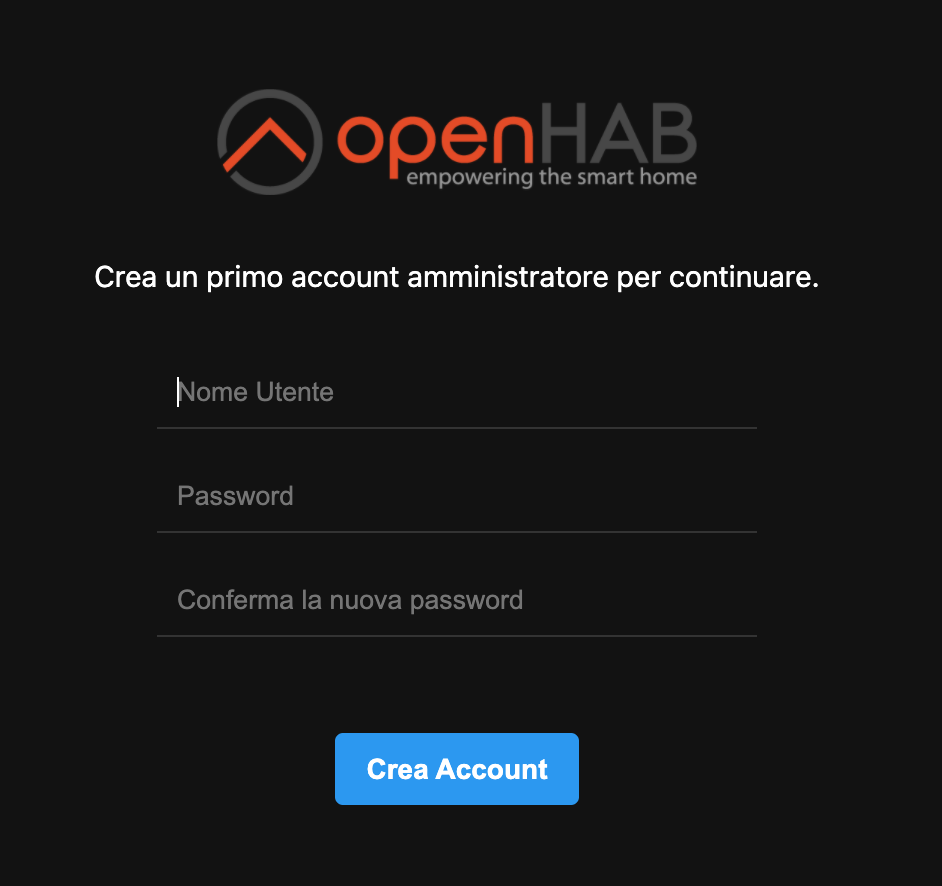
\includegraphics[width=12cm]{Immagini/create_admin}
        \caption{Crea Utente Amministratore}
        \label{fig:create_admin}
    \end{figure}
    \item impostare lingua regione e fuso orario e premere su ``Inizia Installazione'' (Figura \ref{fig:language_region}
    \begin{figure}
        \centering
        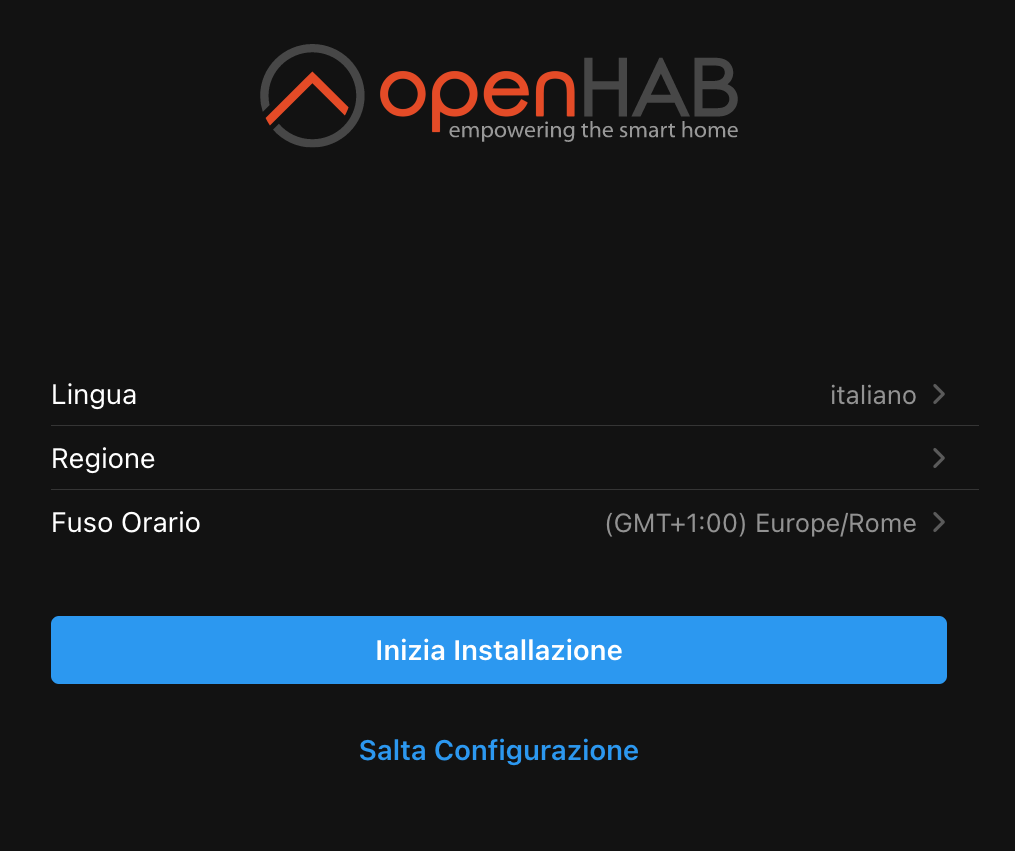
\includegraphics[width=12cm]{Immagini/language_region}
        \caption{Impostazione Lingua Regione e Fuso orario}
        \label{fig:language_region}
    \end{figure}
    \item impostare la posizione (Figura \ref{fig:location})
    \begin{figure}
        \centering
        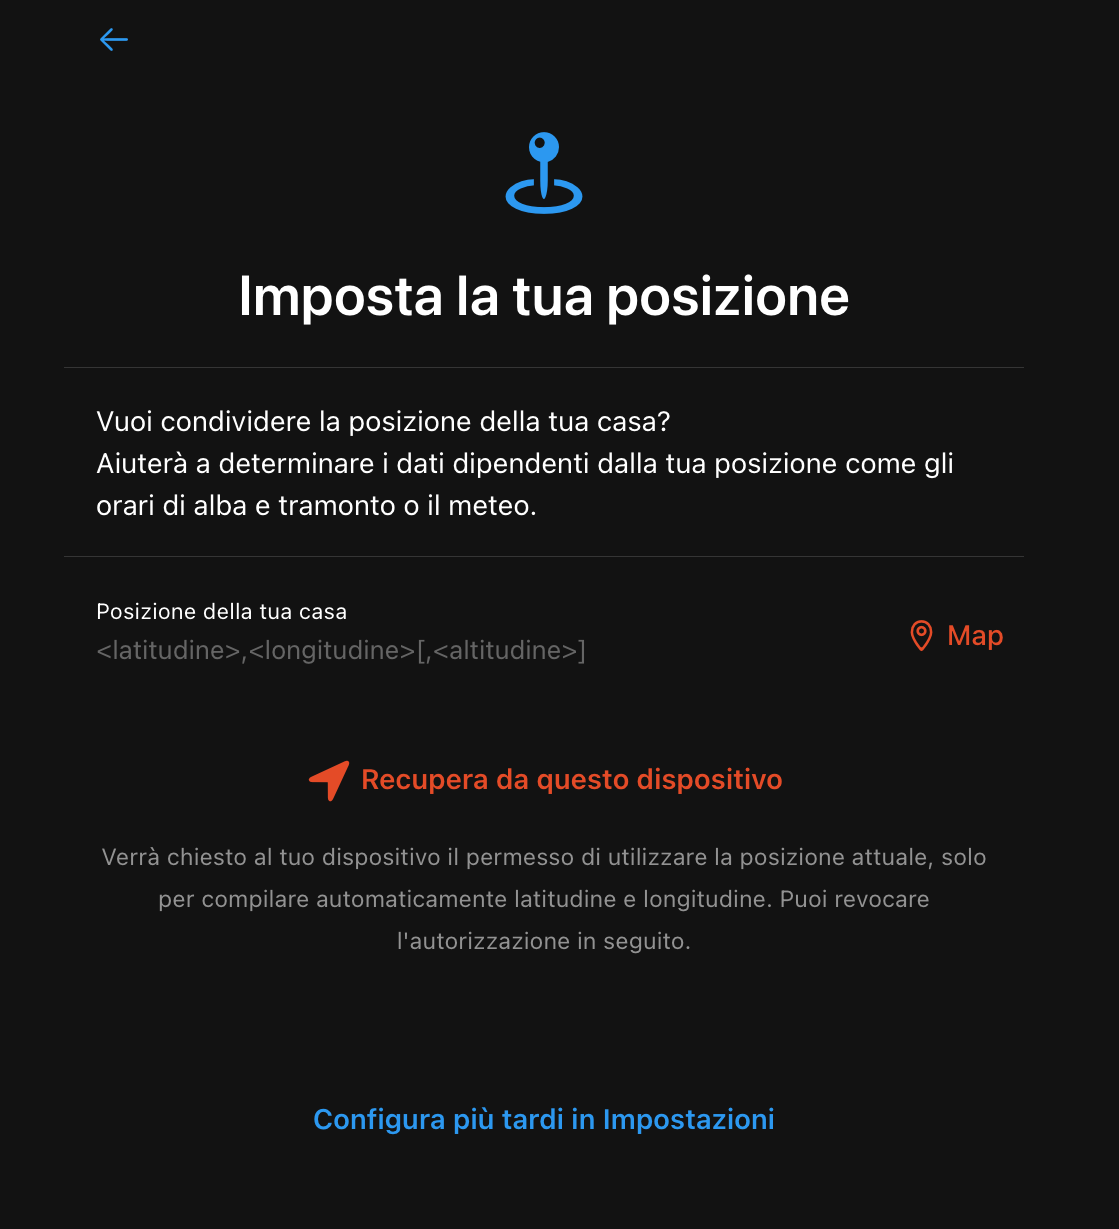
\includegraphics[width=12cm]{Immagini/location}
        \caption{Impostazione Posizione}
        \label{fig:location}
    \end{figure}
    \item installare Add-on, in questo caso \'e stato selezionato il binding MQTT. Per fare ci\'o basta premere la scritta ``Seleziona gli add-on da installare'' e selezionare \textbf{MQTT Binding}. Finita tale procedura premere su ``Installa 1 add-on'' per continuare (Figura \ref{fig:add_on})
    \begin{figure}
        \centering
        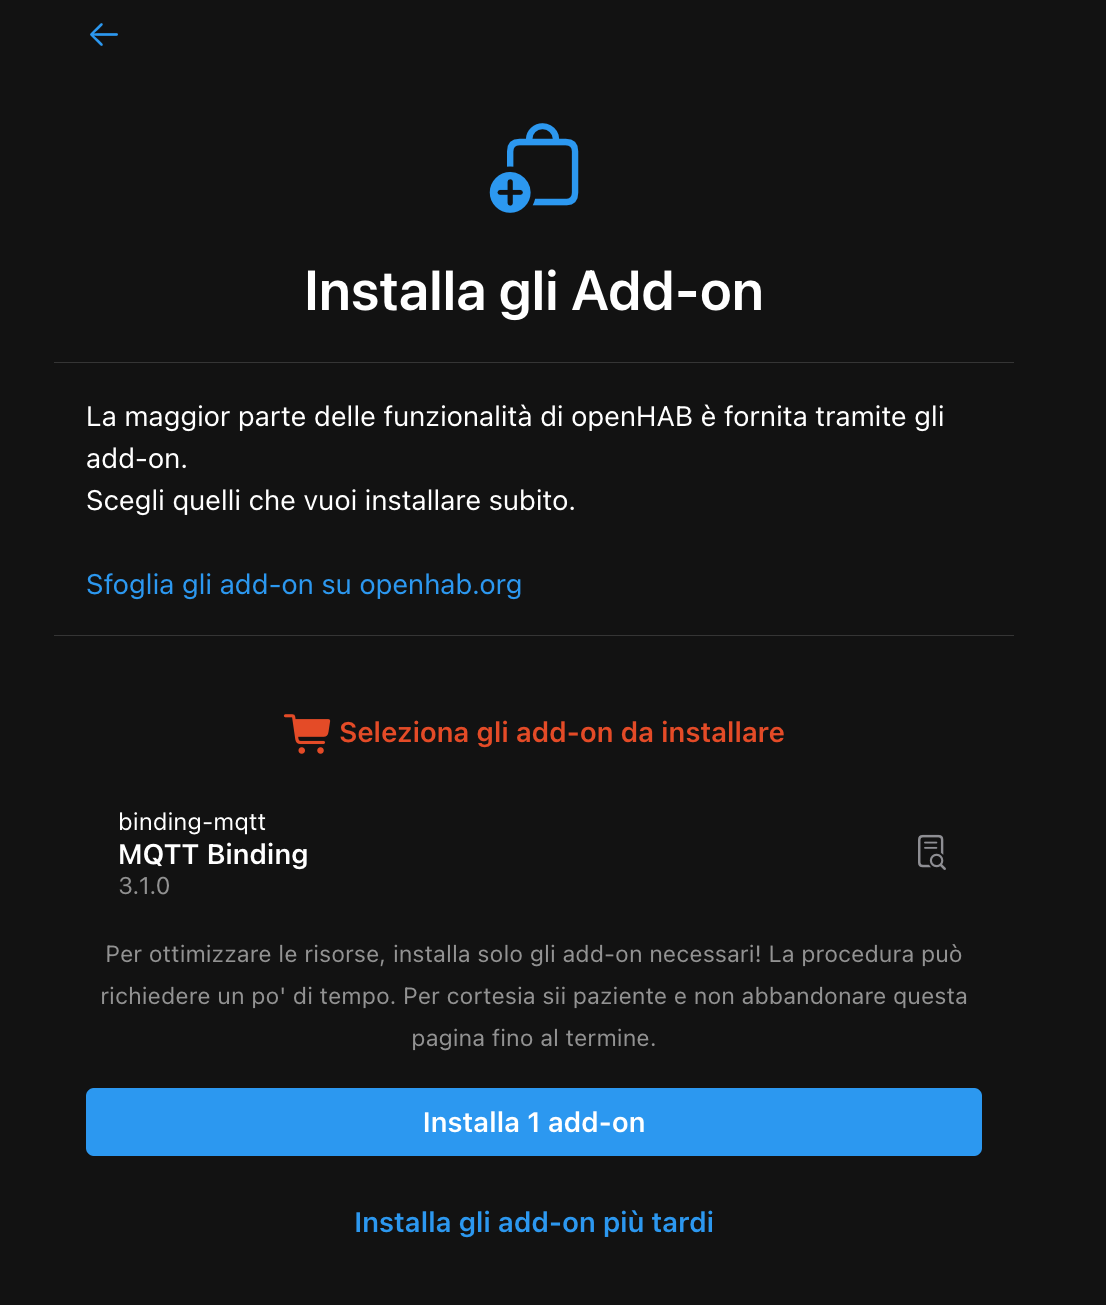
\includegraphics[width=12cm]{Immagini/add_on}
        \caption{Selezionare Add-ons}
        \label{fig:add_on}
    \end{figure}
    \item premere su ``Cominciamo''
\end{enumerate}

\subsection{MQTT Binding di openHAB}
Eseguita la configurazione iniziale ora passiamo a configurare il Binding MQTT per collegare openHAB allo Smart Garden. I passaggi sono i seguenti:
\begin{enumerate}
    \item dalla schermata principale premere su ``Impostazioni'' e successivamente su ``Things'' (Figura \ref{fig:schermata_impostazioni})
    \begin{figure}
        \centering
        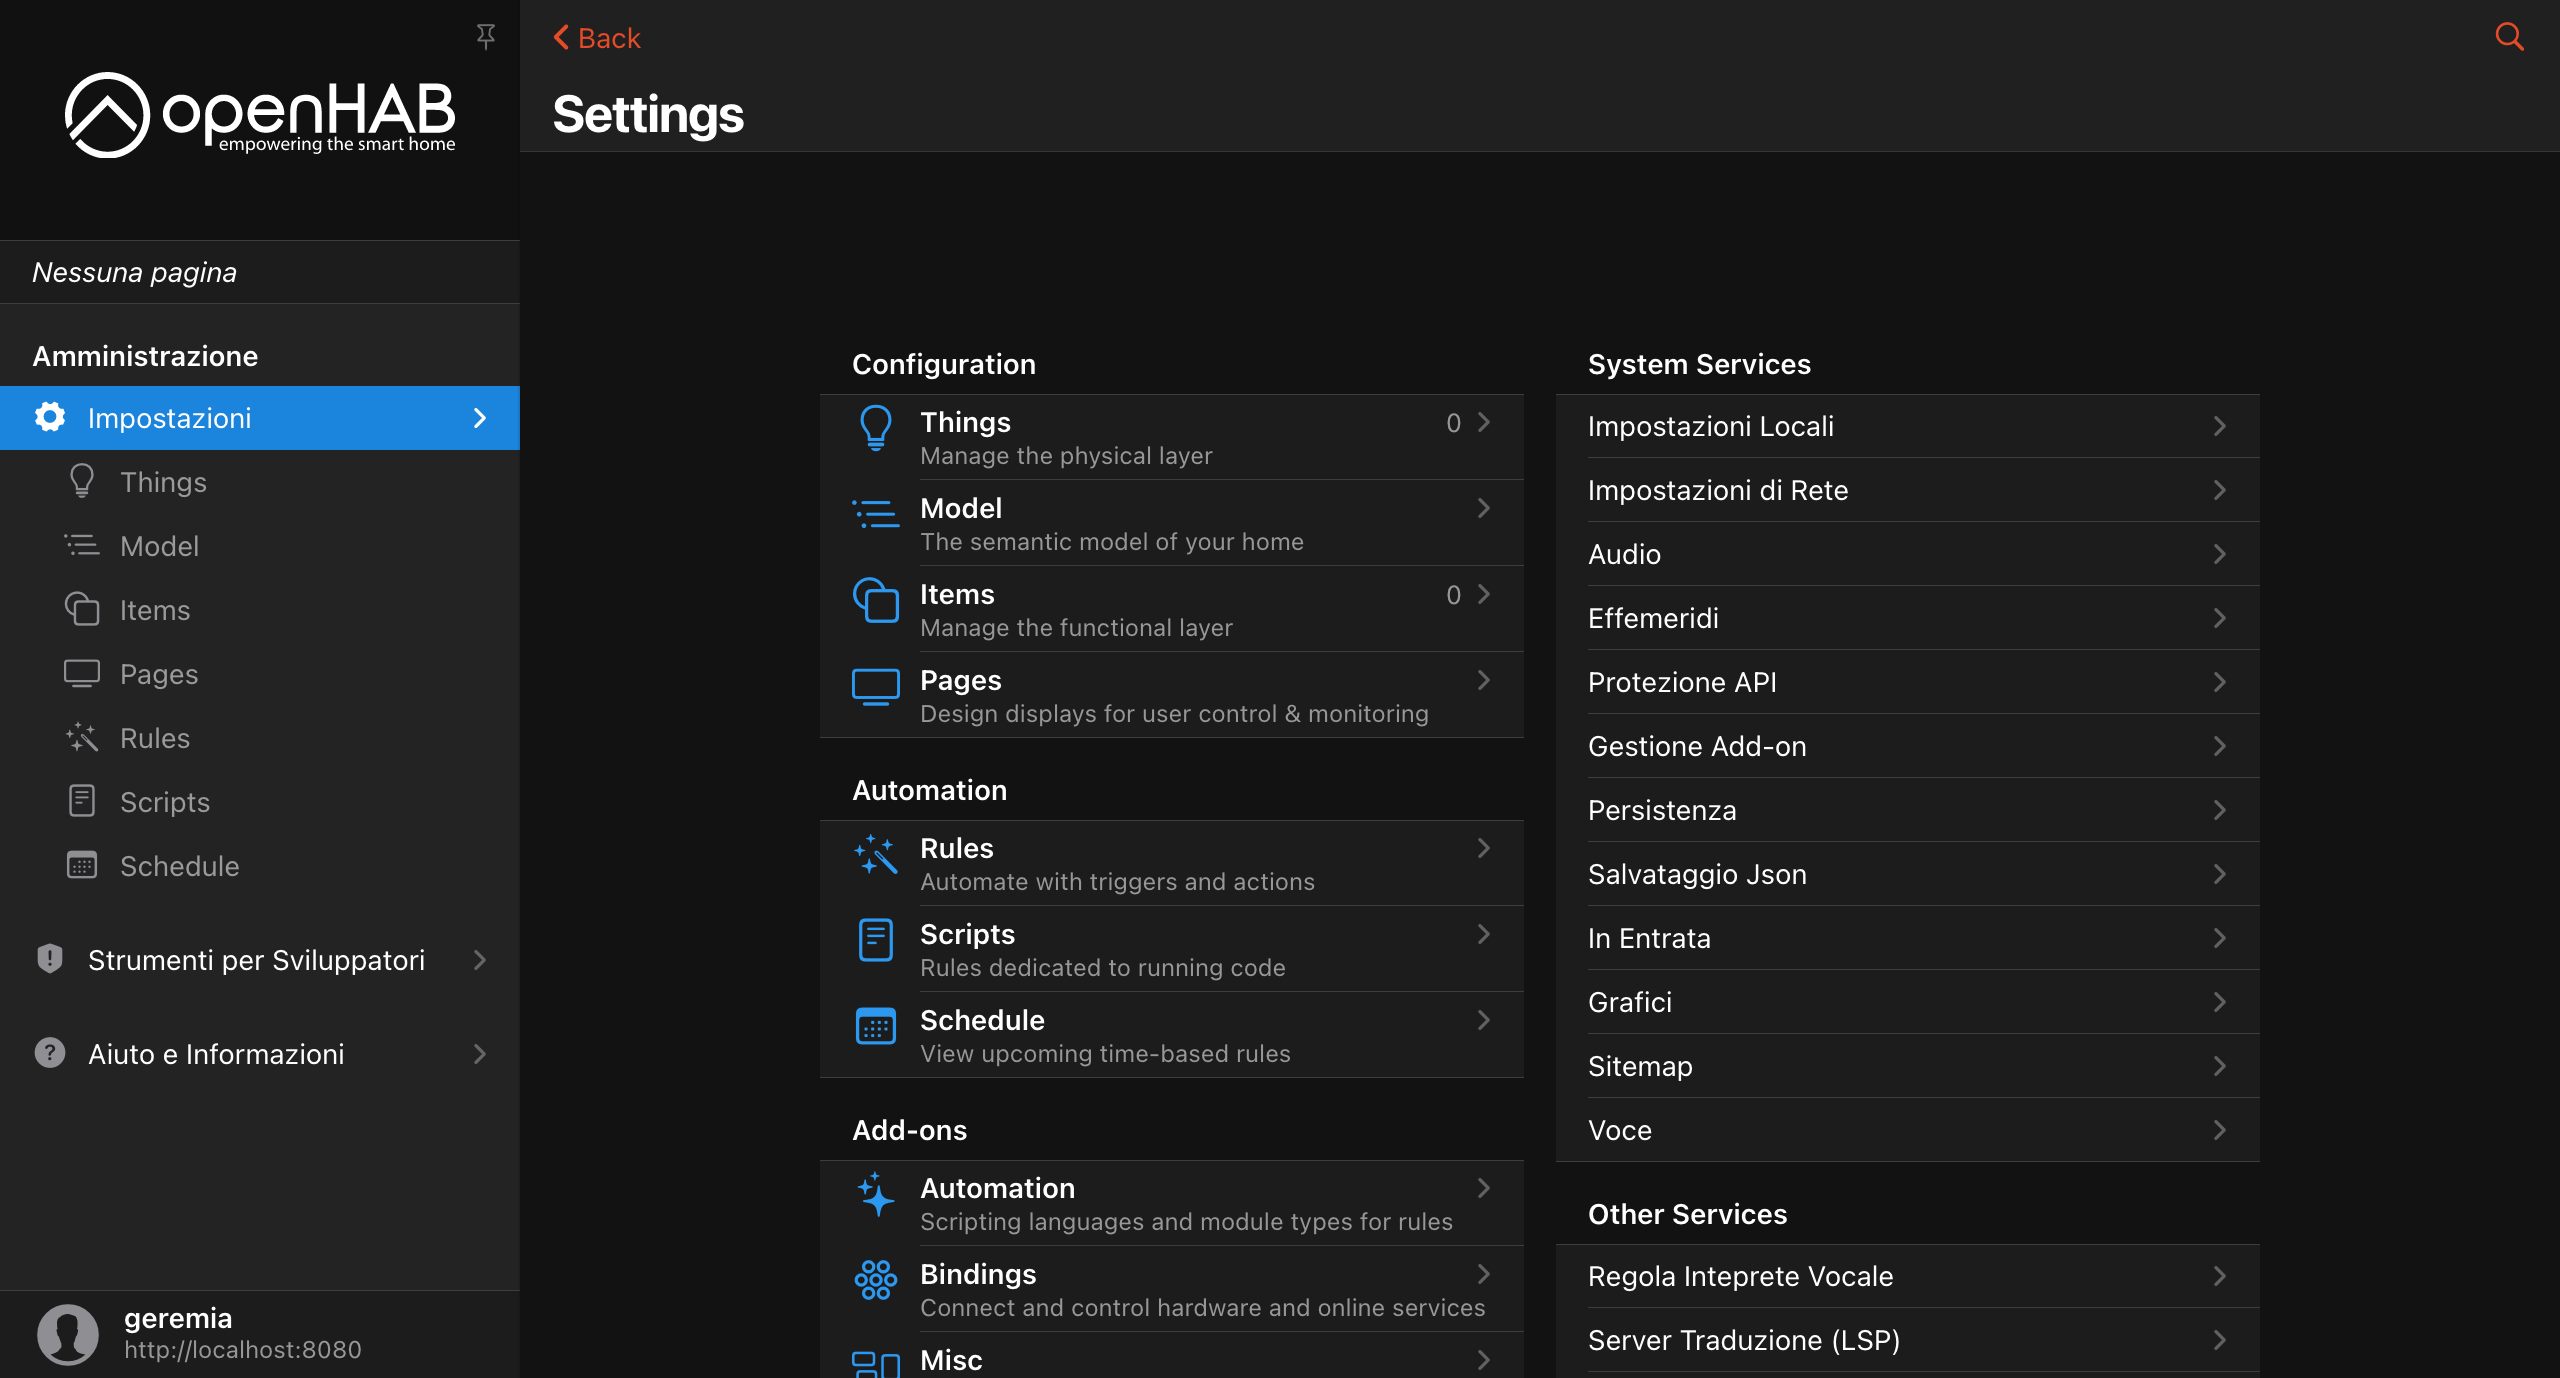
\includegraphics[width=12cm]{Immagini/schermata_impostazioni}
        \caption{Schermata Impostazioni}
        \label{fig:schermata_impostazioni}
    \end{figure}
    \item \label{enum:plus} premere sul ``+'' in basso a destra per scegliere un binding (Figura \ref{fig:schermata_things})
    \begin{figure}
        \centering
        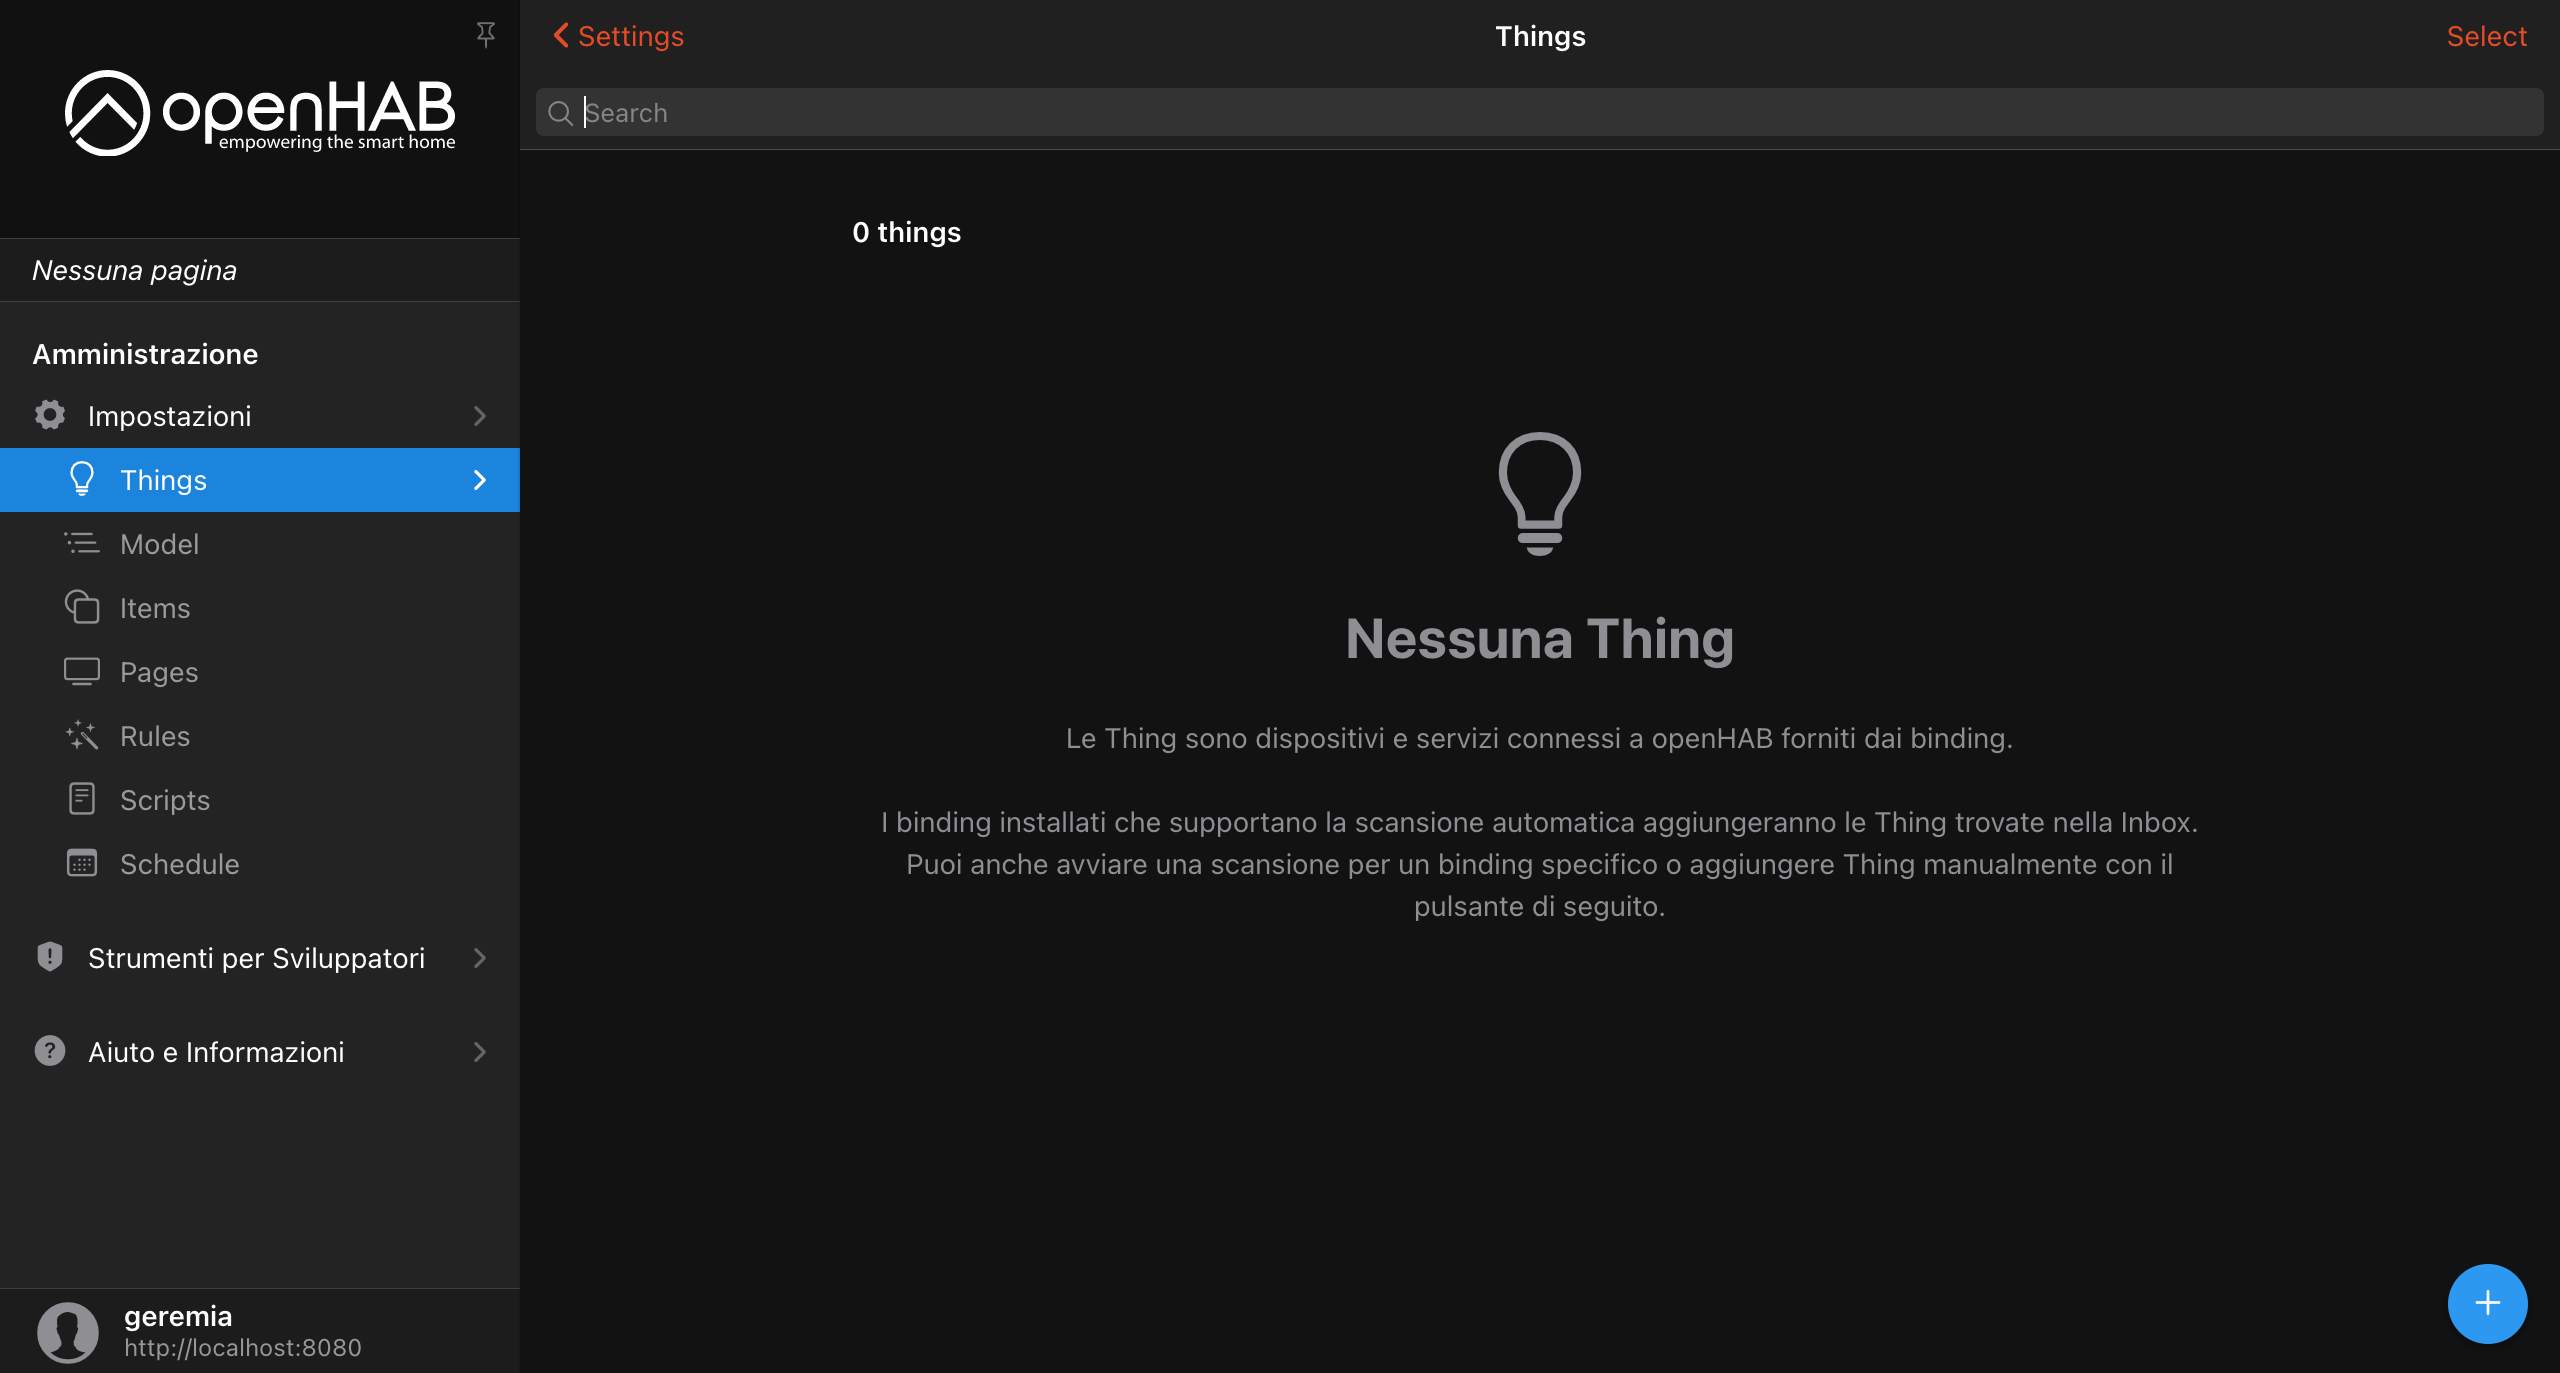
\includegraphics[width=12cm]{Immagini/schermata_things}
        \caption{Schermata Things}
        \label{fig:schermata_things}
    \end{figure}
    \item \label{enum:mqtt_binding}  scegliere il ``MQTT binding'' (Figura \ref{fig:choose_binding})
    \begin{figure}
        \centering
        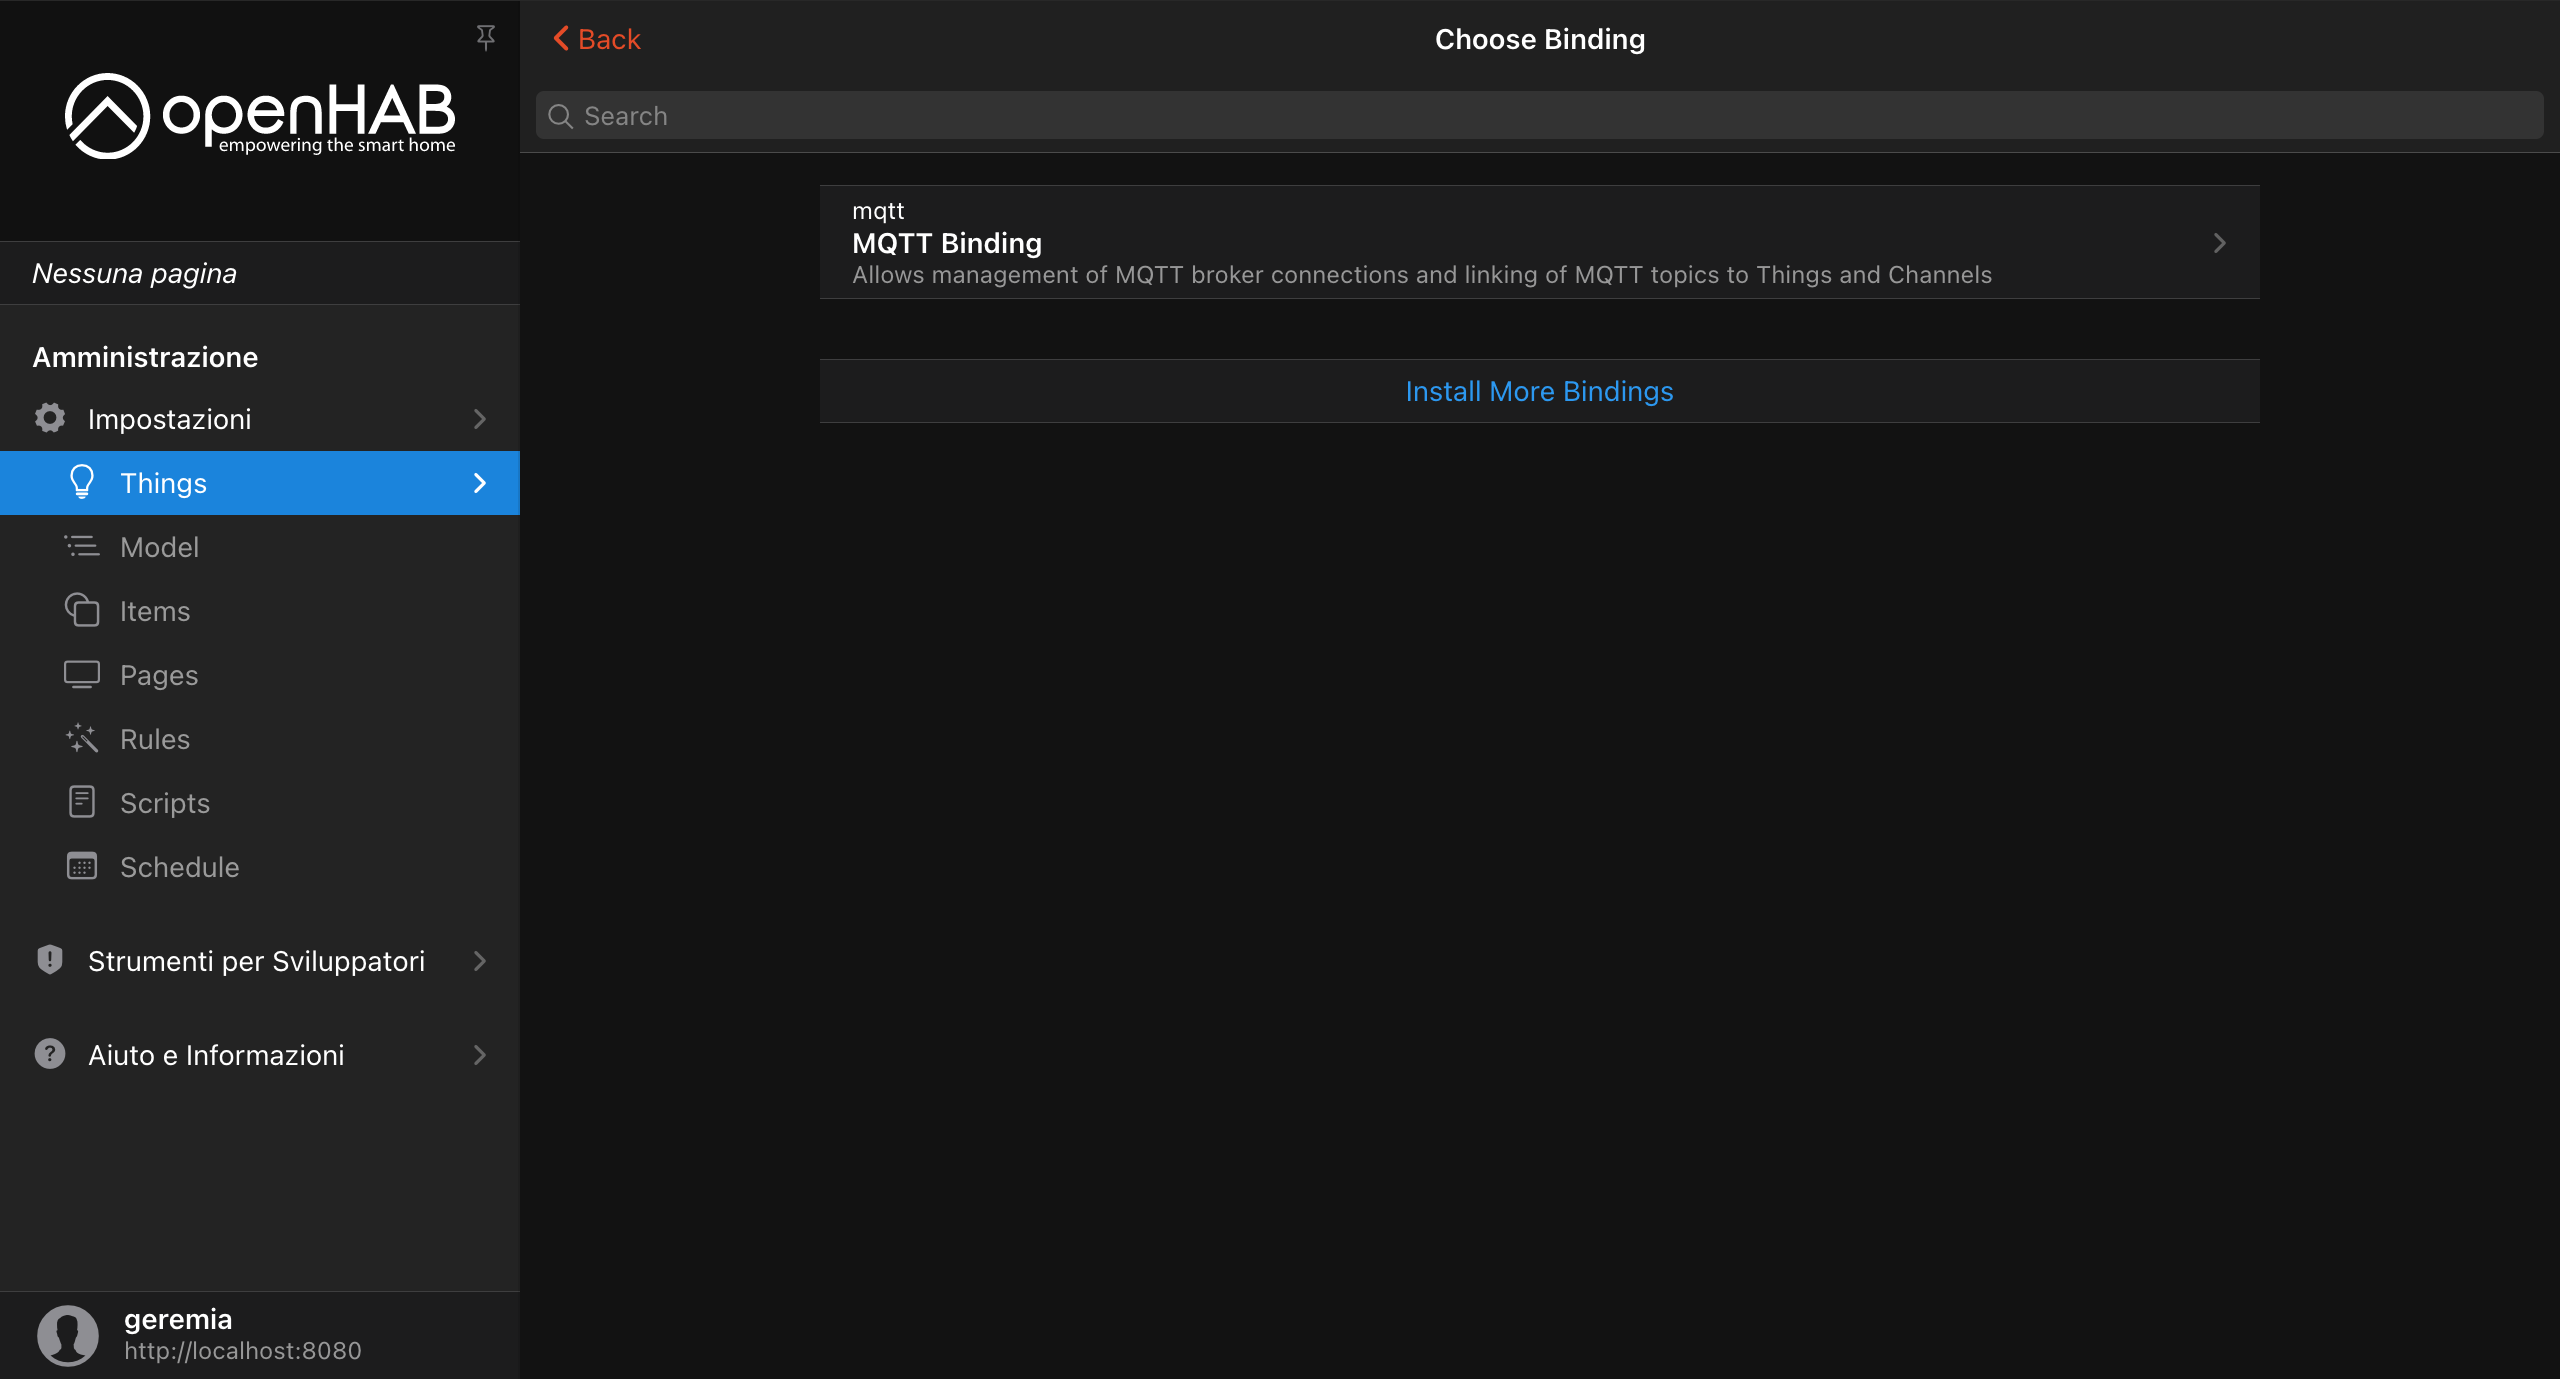
\includegraphics[width=12cm]{Immagini/choose_binding}
        \caption{Schermata Scelta Binding}
        \label{fig:choose_binding}
    \end{figure}
    \item aggiungere la thing ``MQTT Broker'' (Figura \ref{fig:add_new_thing})
    \begin{figure}
        \centering
        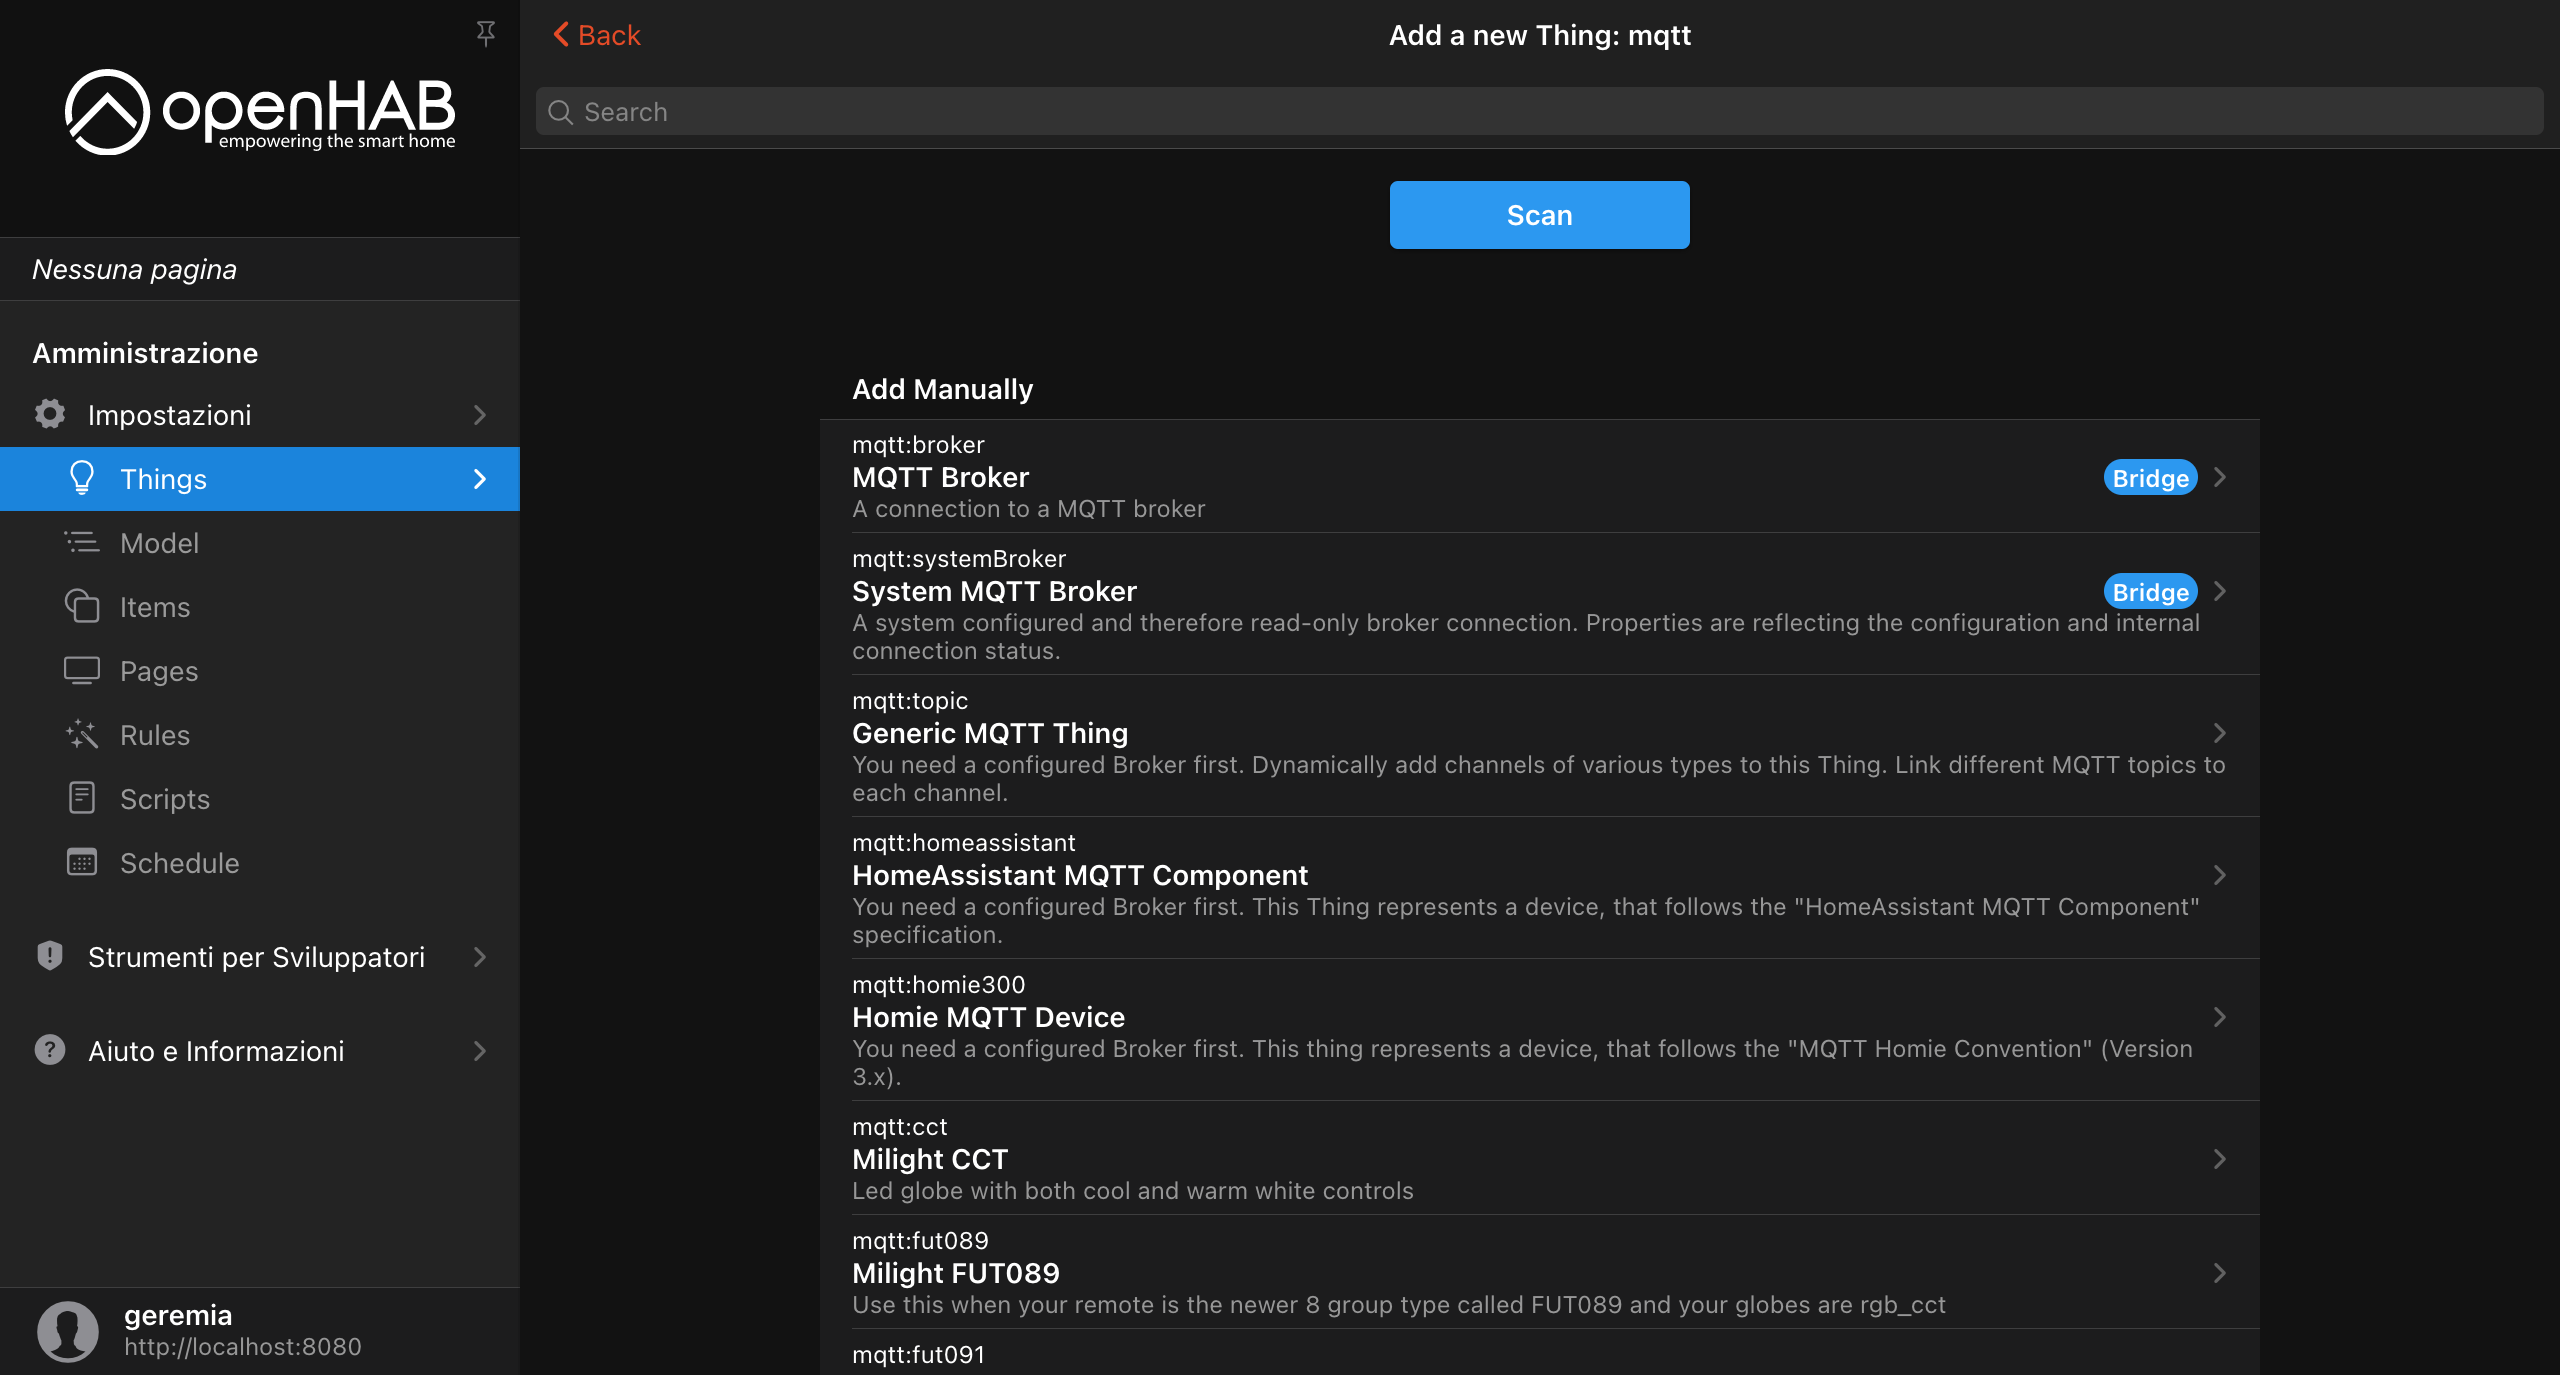
\includegraphics[width=12cm]{Immagini/add_new_thing}
        \caption{Schermata aggiunta Thing}
        \label{fig:add_new_thing}
    \end{figure}
    \item \label{enum:mqtt_broker} configurare {\em MQTT Broker} aggiungendo {\em Broker Hostname/IP} (IP del broker MQTT) e premendo sul pulsante ``Create Thing'' (in tal caso verr\'a aggiunto l'indirizzo IP locale della Raspberry Pi che ha gi\'a mosquitto installato). Appena eseguita tale operazione si ritorner\'a alla schermata precedente con la nuova thing aggiunta. In tale schermata \'e possibile visualizzare se lo stato del broker MQTT \'e ONLINE o OFFLINE 
    (Figura \ref{fig:mqtt_broker_config})
    \begin{figure}
        \centering
        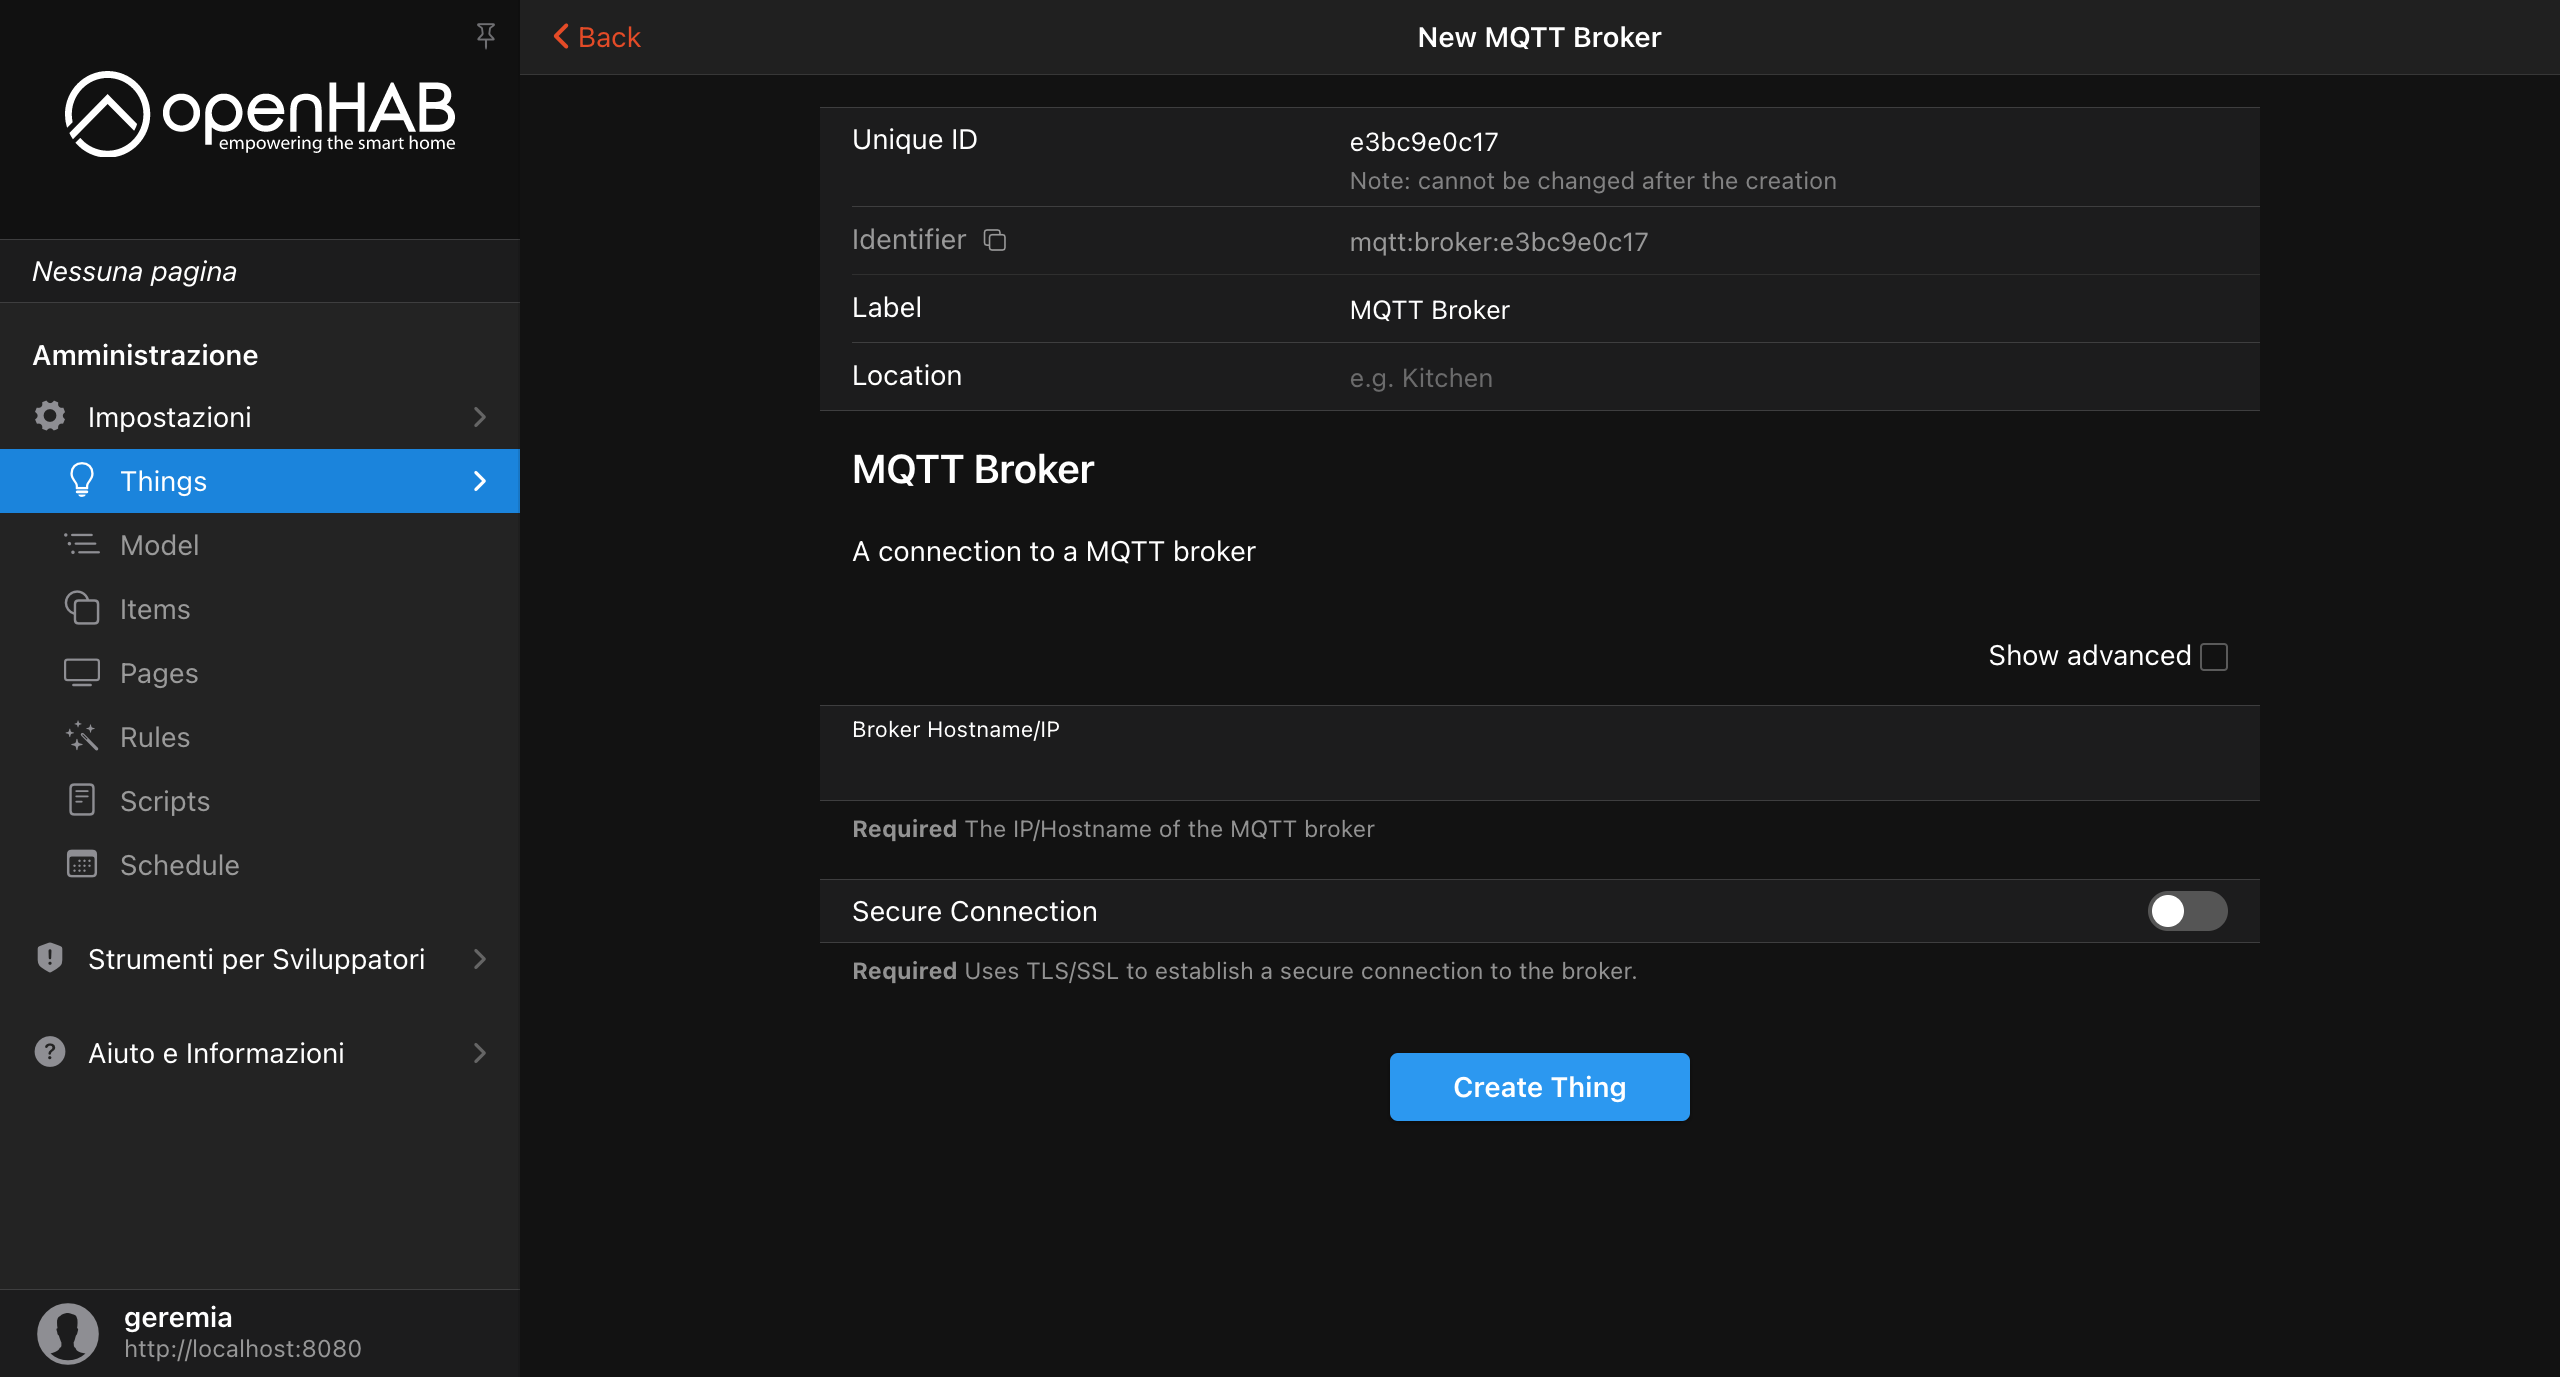
\includegraphics[width=12cm]{Immagini/mqtt_broker_config}
        \caption{Configurazione MQTT Broker}
        \label{fig:mqtt_broker_config}
    \end{figure}
    \item aggiungere un ulterioire thing rieseguendo i passaggi \ref{enum:plus} e \ref{enum:mqtt_binding} e selezionando questa volta la voce ``Generic MQTT Thing''
    \item si procede alla configurazione aggiungendo i campi:
    \begin{itemize}
        \item \textbf{Label}: rinominarlo con un nome mnemonico cos\'i da rendere pi\'u semplice la sua ricerca futura (in questo caso ``Samrt Garden'')
        \item \textbf{Location}: aggiungere la posizione nella casa della nuova thing (in questo caso ``Garden'')
        \item \textbf{Bridge}: selezionare ``MQTT Broker'', ovvero la thing aggiunta al passaggio \ref{enum:mqtt_broker}
    \end{itemize}
    premere infine su ``Create Thing'' (Figura \ref{fig:mqtt_thing_config})
    \begin{figure}
        \centering
        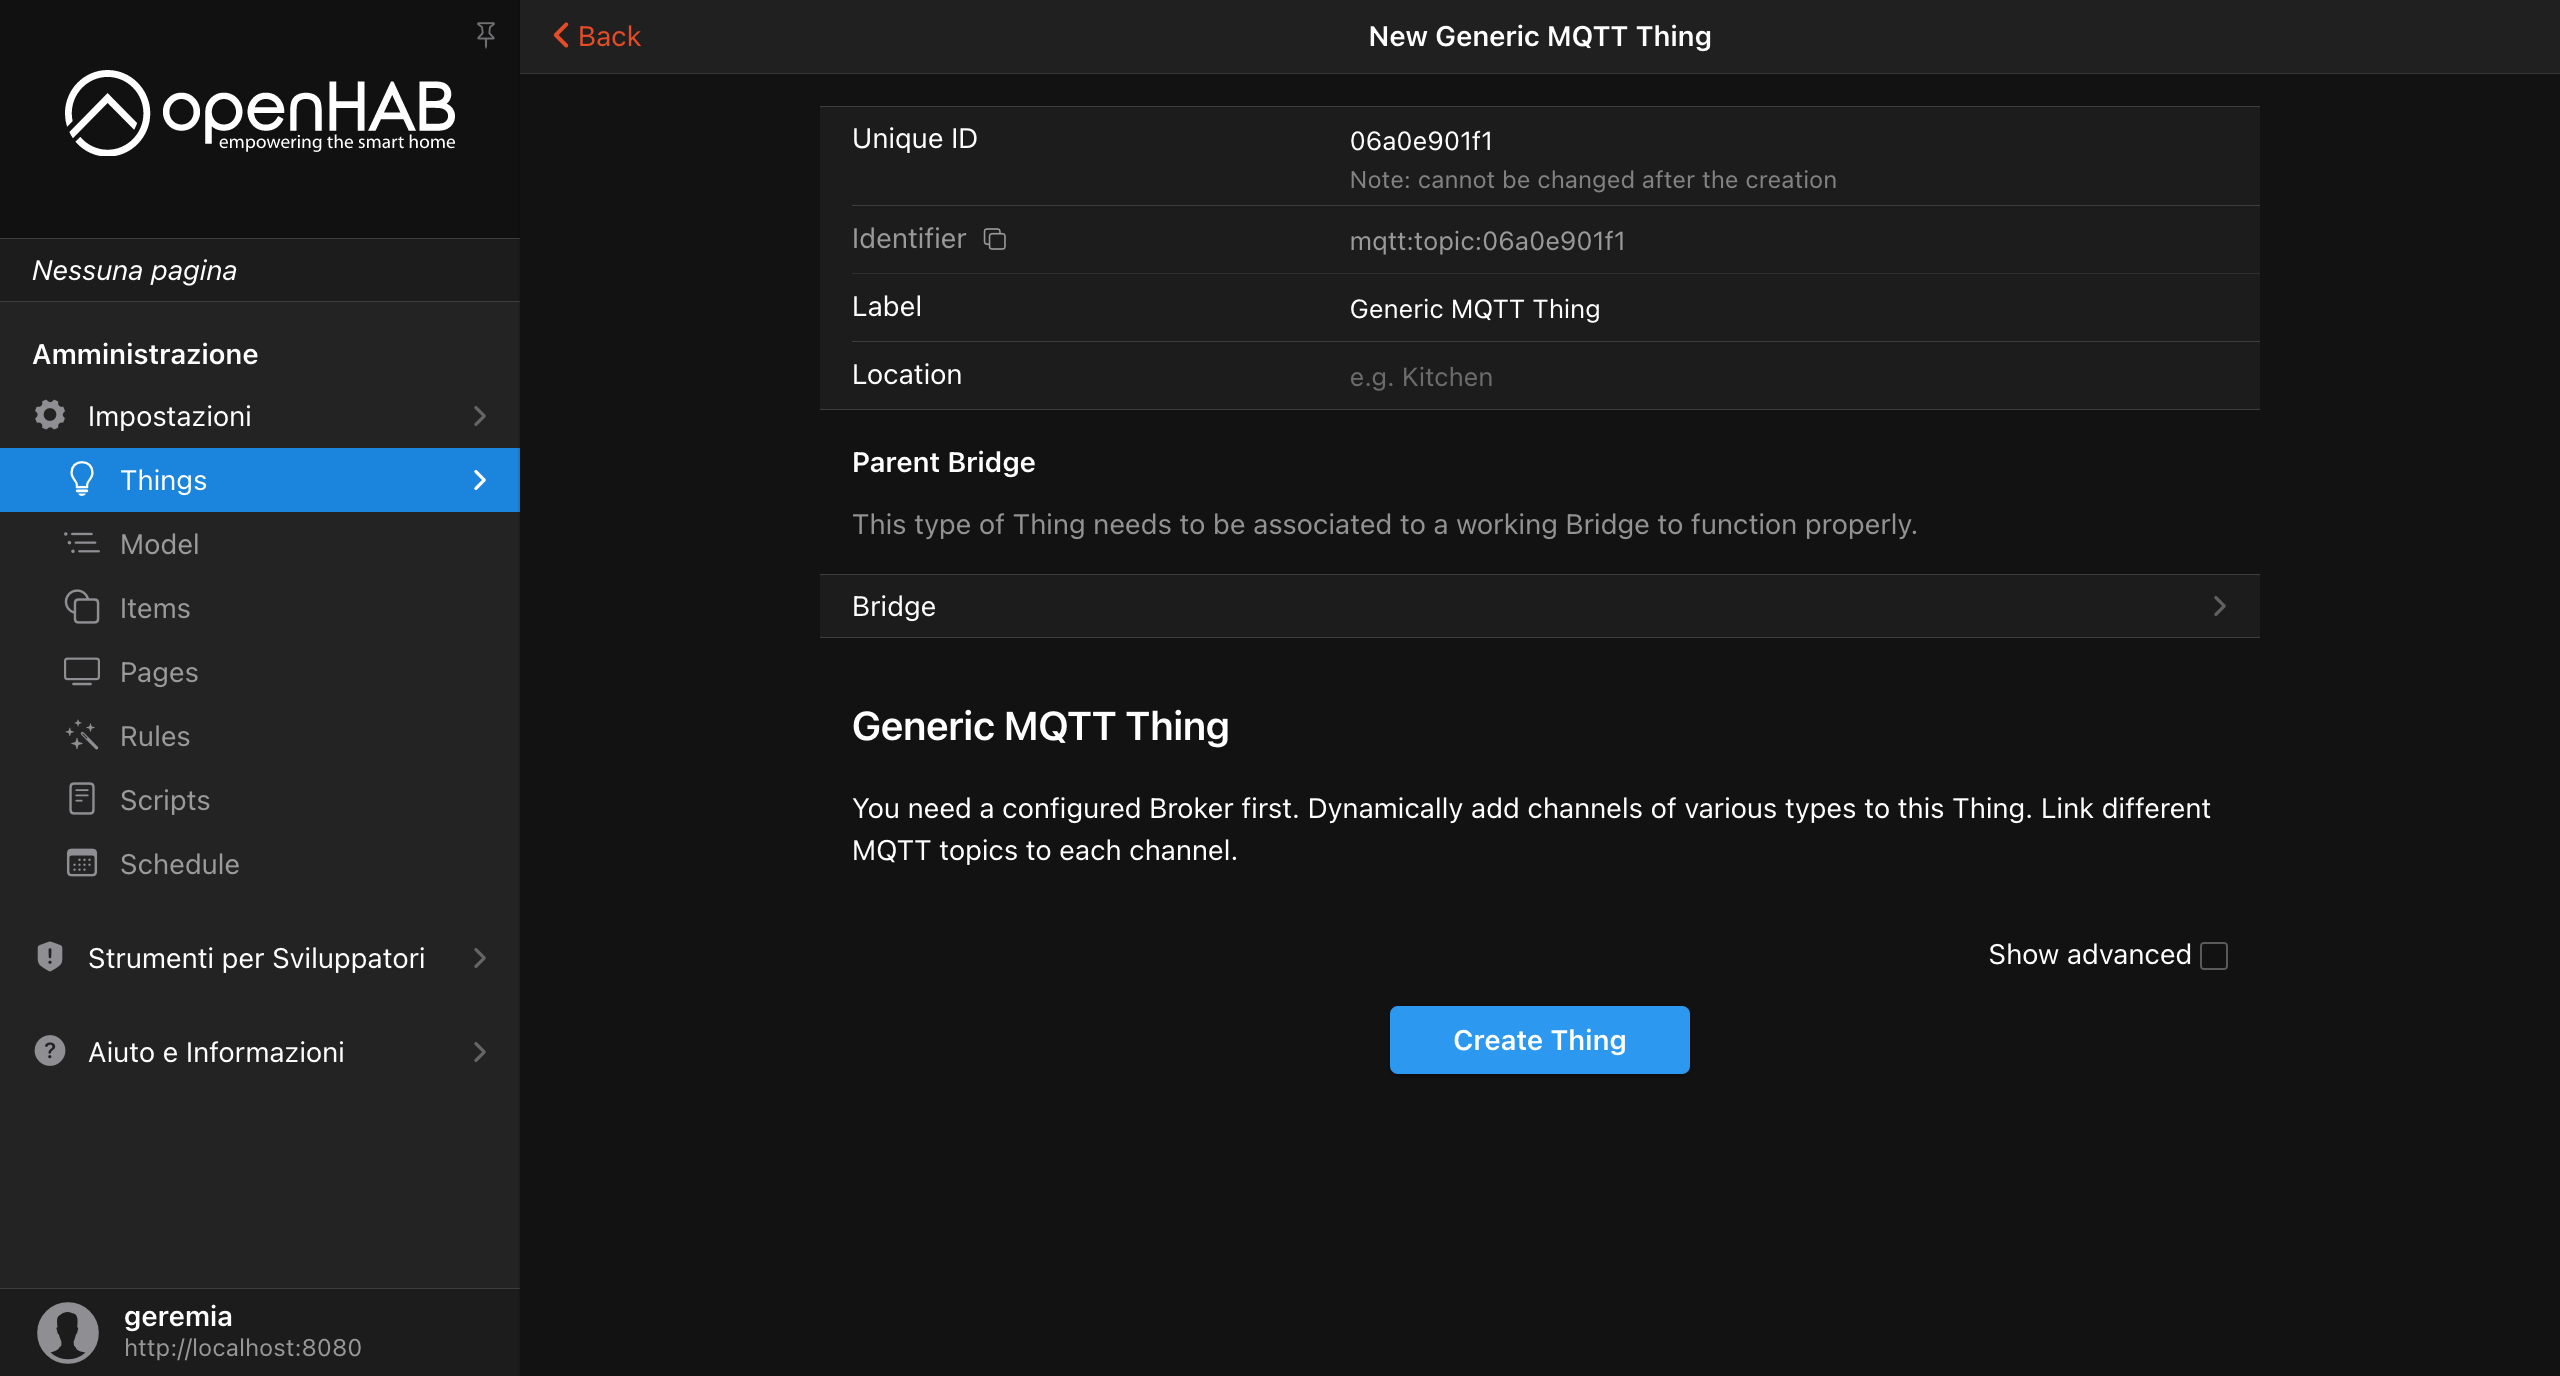
\includegraphics[width=12cm]{Immagini/mqtt_thing_config}
        \caption{Configurazione MQTT Thing}
        \label{fig:mqtt_thing_config}
    \end{figure}
    \item ritornati alla schermata Things, a questo punto bisogna aggiungere i Channels relativi ai topic MQTT all'interno della thing appena creata. Quindi premere sulla nuova thing (in questo caso chiamata ``Smart Garden'') e successivamente su Channels. Nella schermata della thing \'e possibile visualizzare il suo status (Figura: \ref{fig:mqtt_thing_smart_garden})
    \begin{figure}
        \centering
        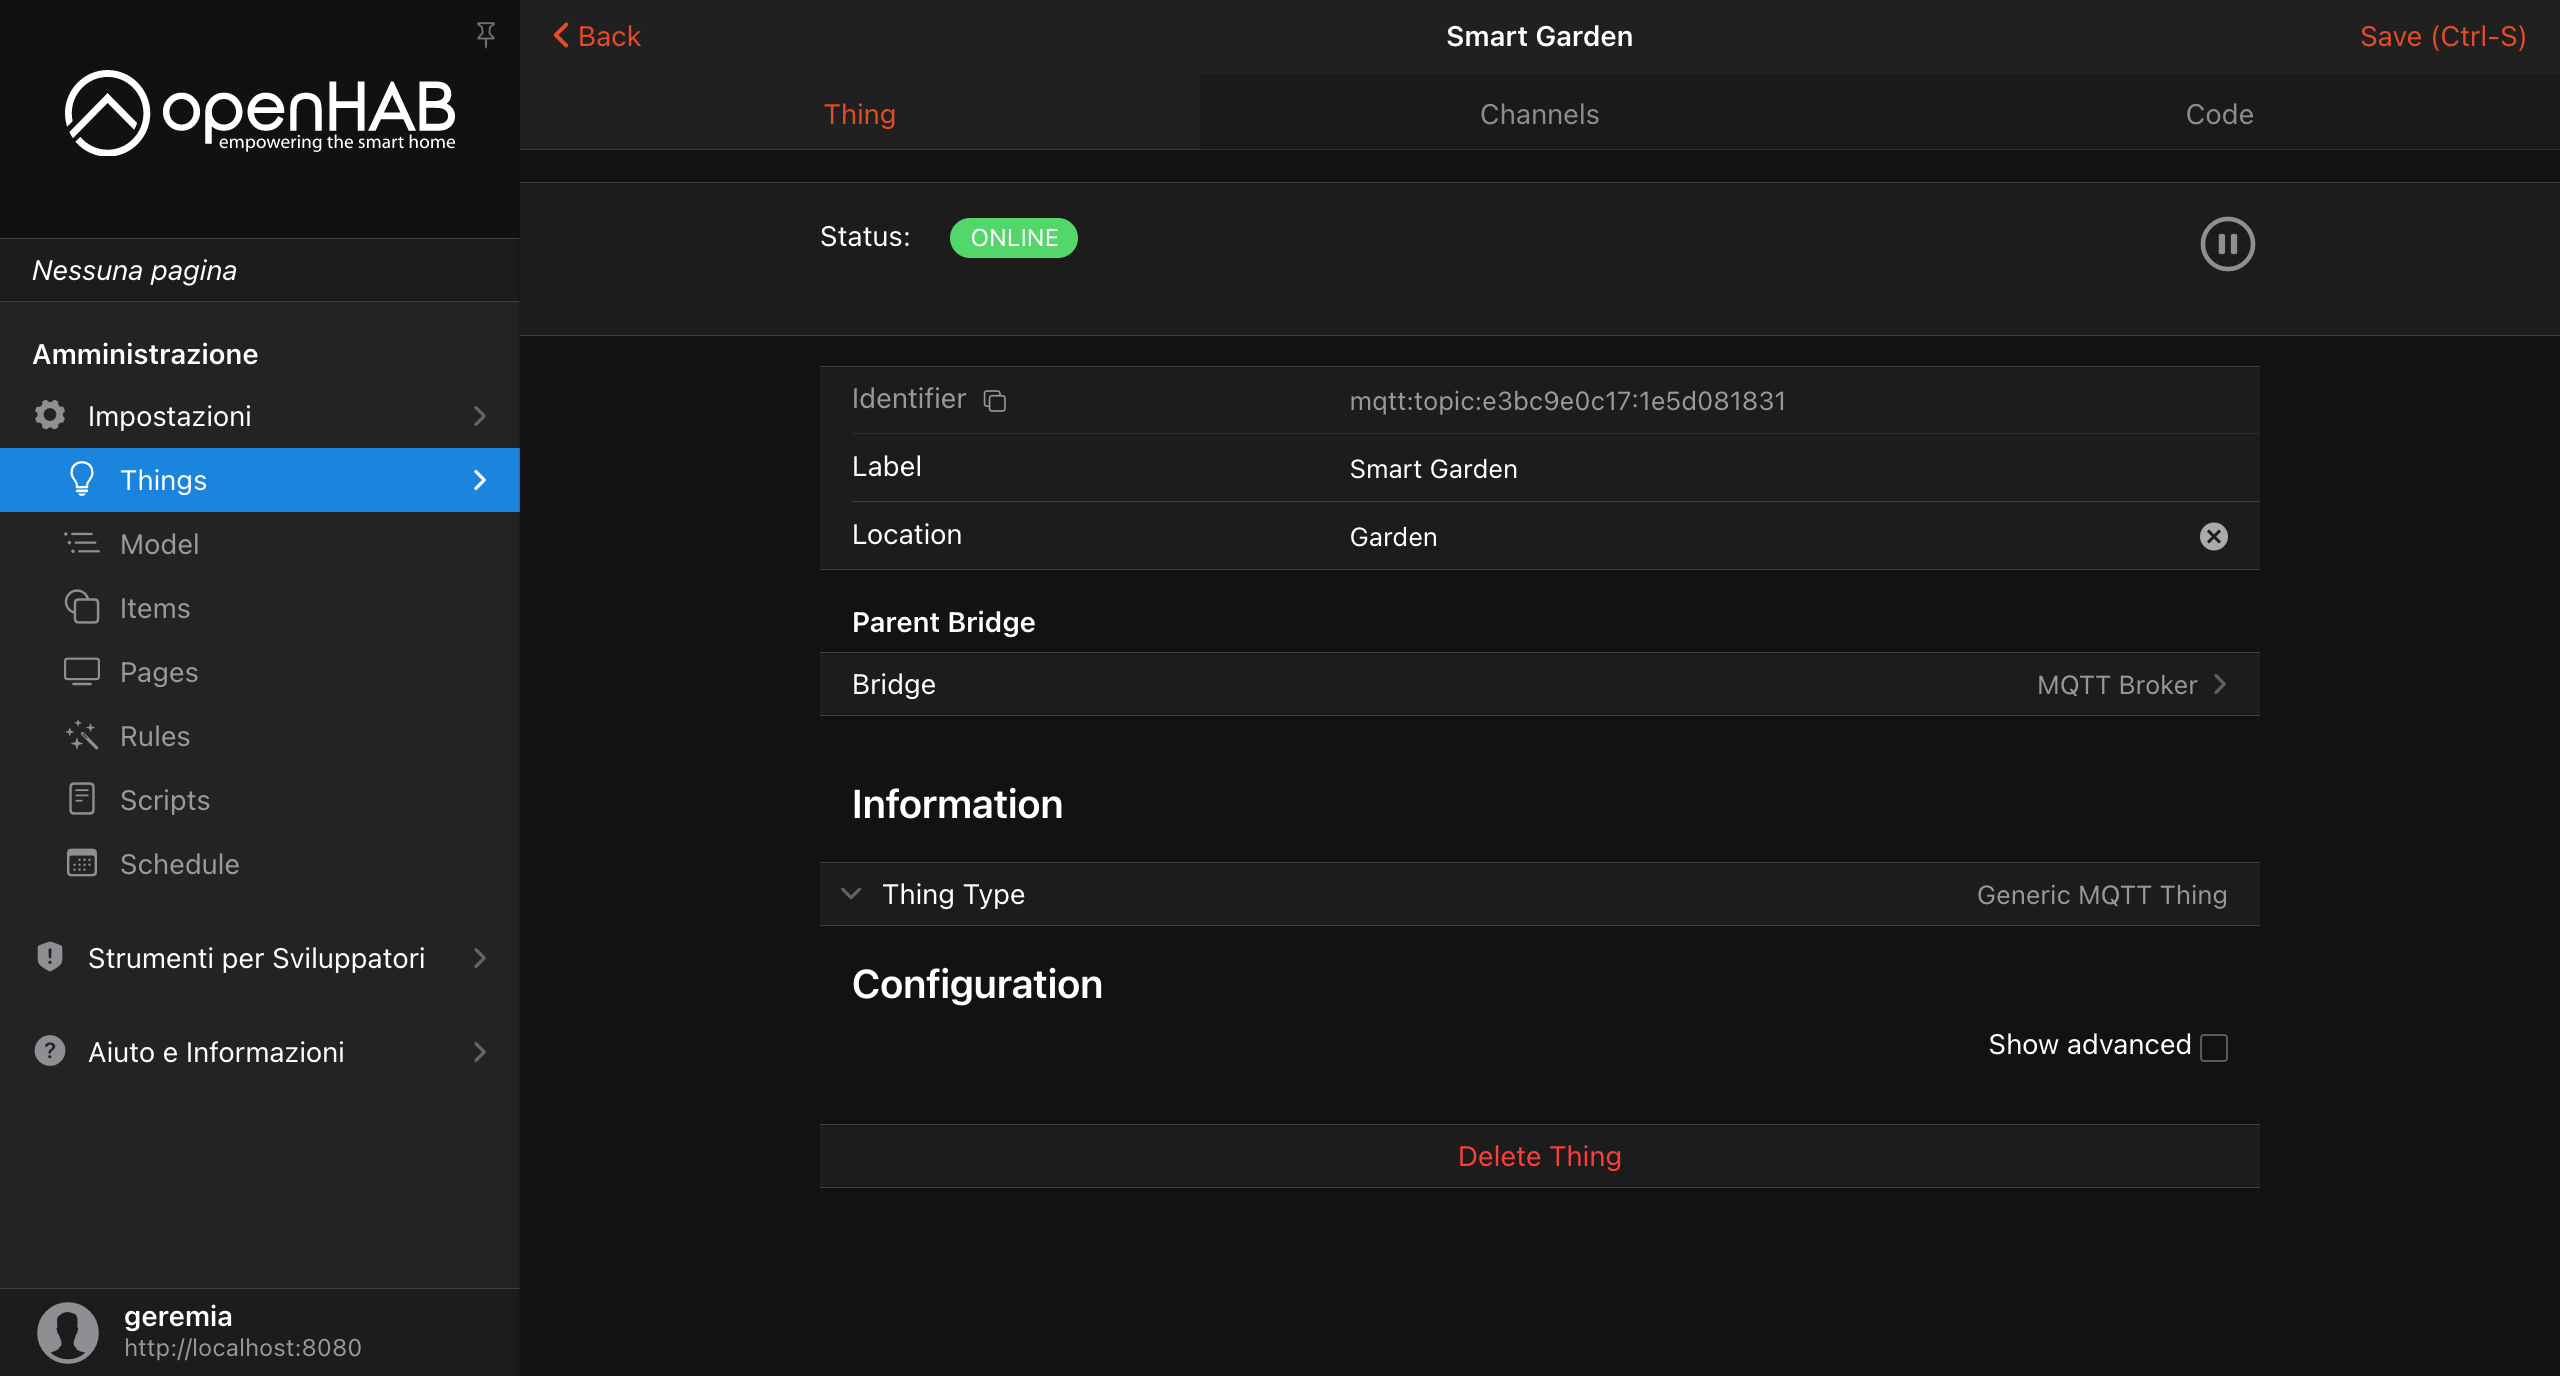
\includegraphics[width=12cm]{Immagini/mqtt_thing_smart_garden}
        \caption{MQTT Thing}
        \label{fig:mqtt_thing_smart_garden}
    \end{figure}
    \item nella schermata Channels \'e possibile aggiungere diversi canali relativi alla thing selezionata precedentamente. Per fare ci\'o basta premere sul pulsante ``Add Channel'' (Figura \ref{fig:channels}) e configurare il channel da aggiungere inserendo i campi richiesti:
    \begin{itemize}
        \item \textbf{Channel Identifier}: id univoco del channel
        \item \textbf{Label}: nome con cui verr\'a visualizzato a video il canale
        \item \textbf{Channel Type}: tipo del channel. Da questo usciranno fuori poi altri campi relativi alla sua configurazione
    \end{itemize}
    In questo caso sono stati aggiunti 4 channels relativi ad ogni topic(handle\_pump e status\_pump fanno riferimento allo stesso topic in due modi differenti: il primo serve per gestire la pompe in maniera manuale accendendola e spegnendola mentre il secondo per visualizzare il suo stato). Verranno riportati con le relative configurazioni alla Tabella \ref{tab:smart_garden_channels}. In quest'ultima i campi ON e OFF sono relativi solo al tipo ``On/Off Switch'' poich\'e corrispondono alle azioni di accenzione e spegnimento. In tutti i channels pu\'o essere attivata la voce sotto ``Show advanced'' chiamata ``Retained'' per abilitare i messaggi inviati ai relativi topic come mantenuti
    \begin{table}[]
        \centering
        \begin{tabular}{l|l|l|l|l|l}
            \textbf{Identifier} & \textbf{Label} & \textbf{Type} & \textbf{Topic} & \textbf{On} & \textbf{Off} \\
            \hline
            handle\_pump & Handle Pump & On/Off Switch & handle/pump & ON & OFF \\
            handle\_auto & Handle Auto & On/Off Switch & handle/auto & ON & OFF \\
            status\_pump & Status Pump & Text Value & handle/pump & - & - \\
            status\_soil & Status Soil & Text Value & status/soil & - & - \\
        \end{tabular}
        \caption{Smart Garden CHannels}
        \label{tab:smart_garden_channels}
    \end{table}
    (Figura \ref{fig:add_channel})
    \begin{figure}
        \centering
        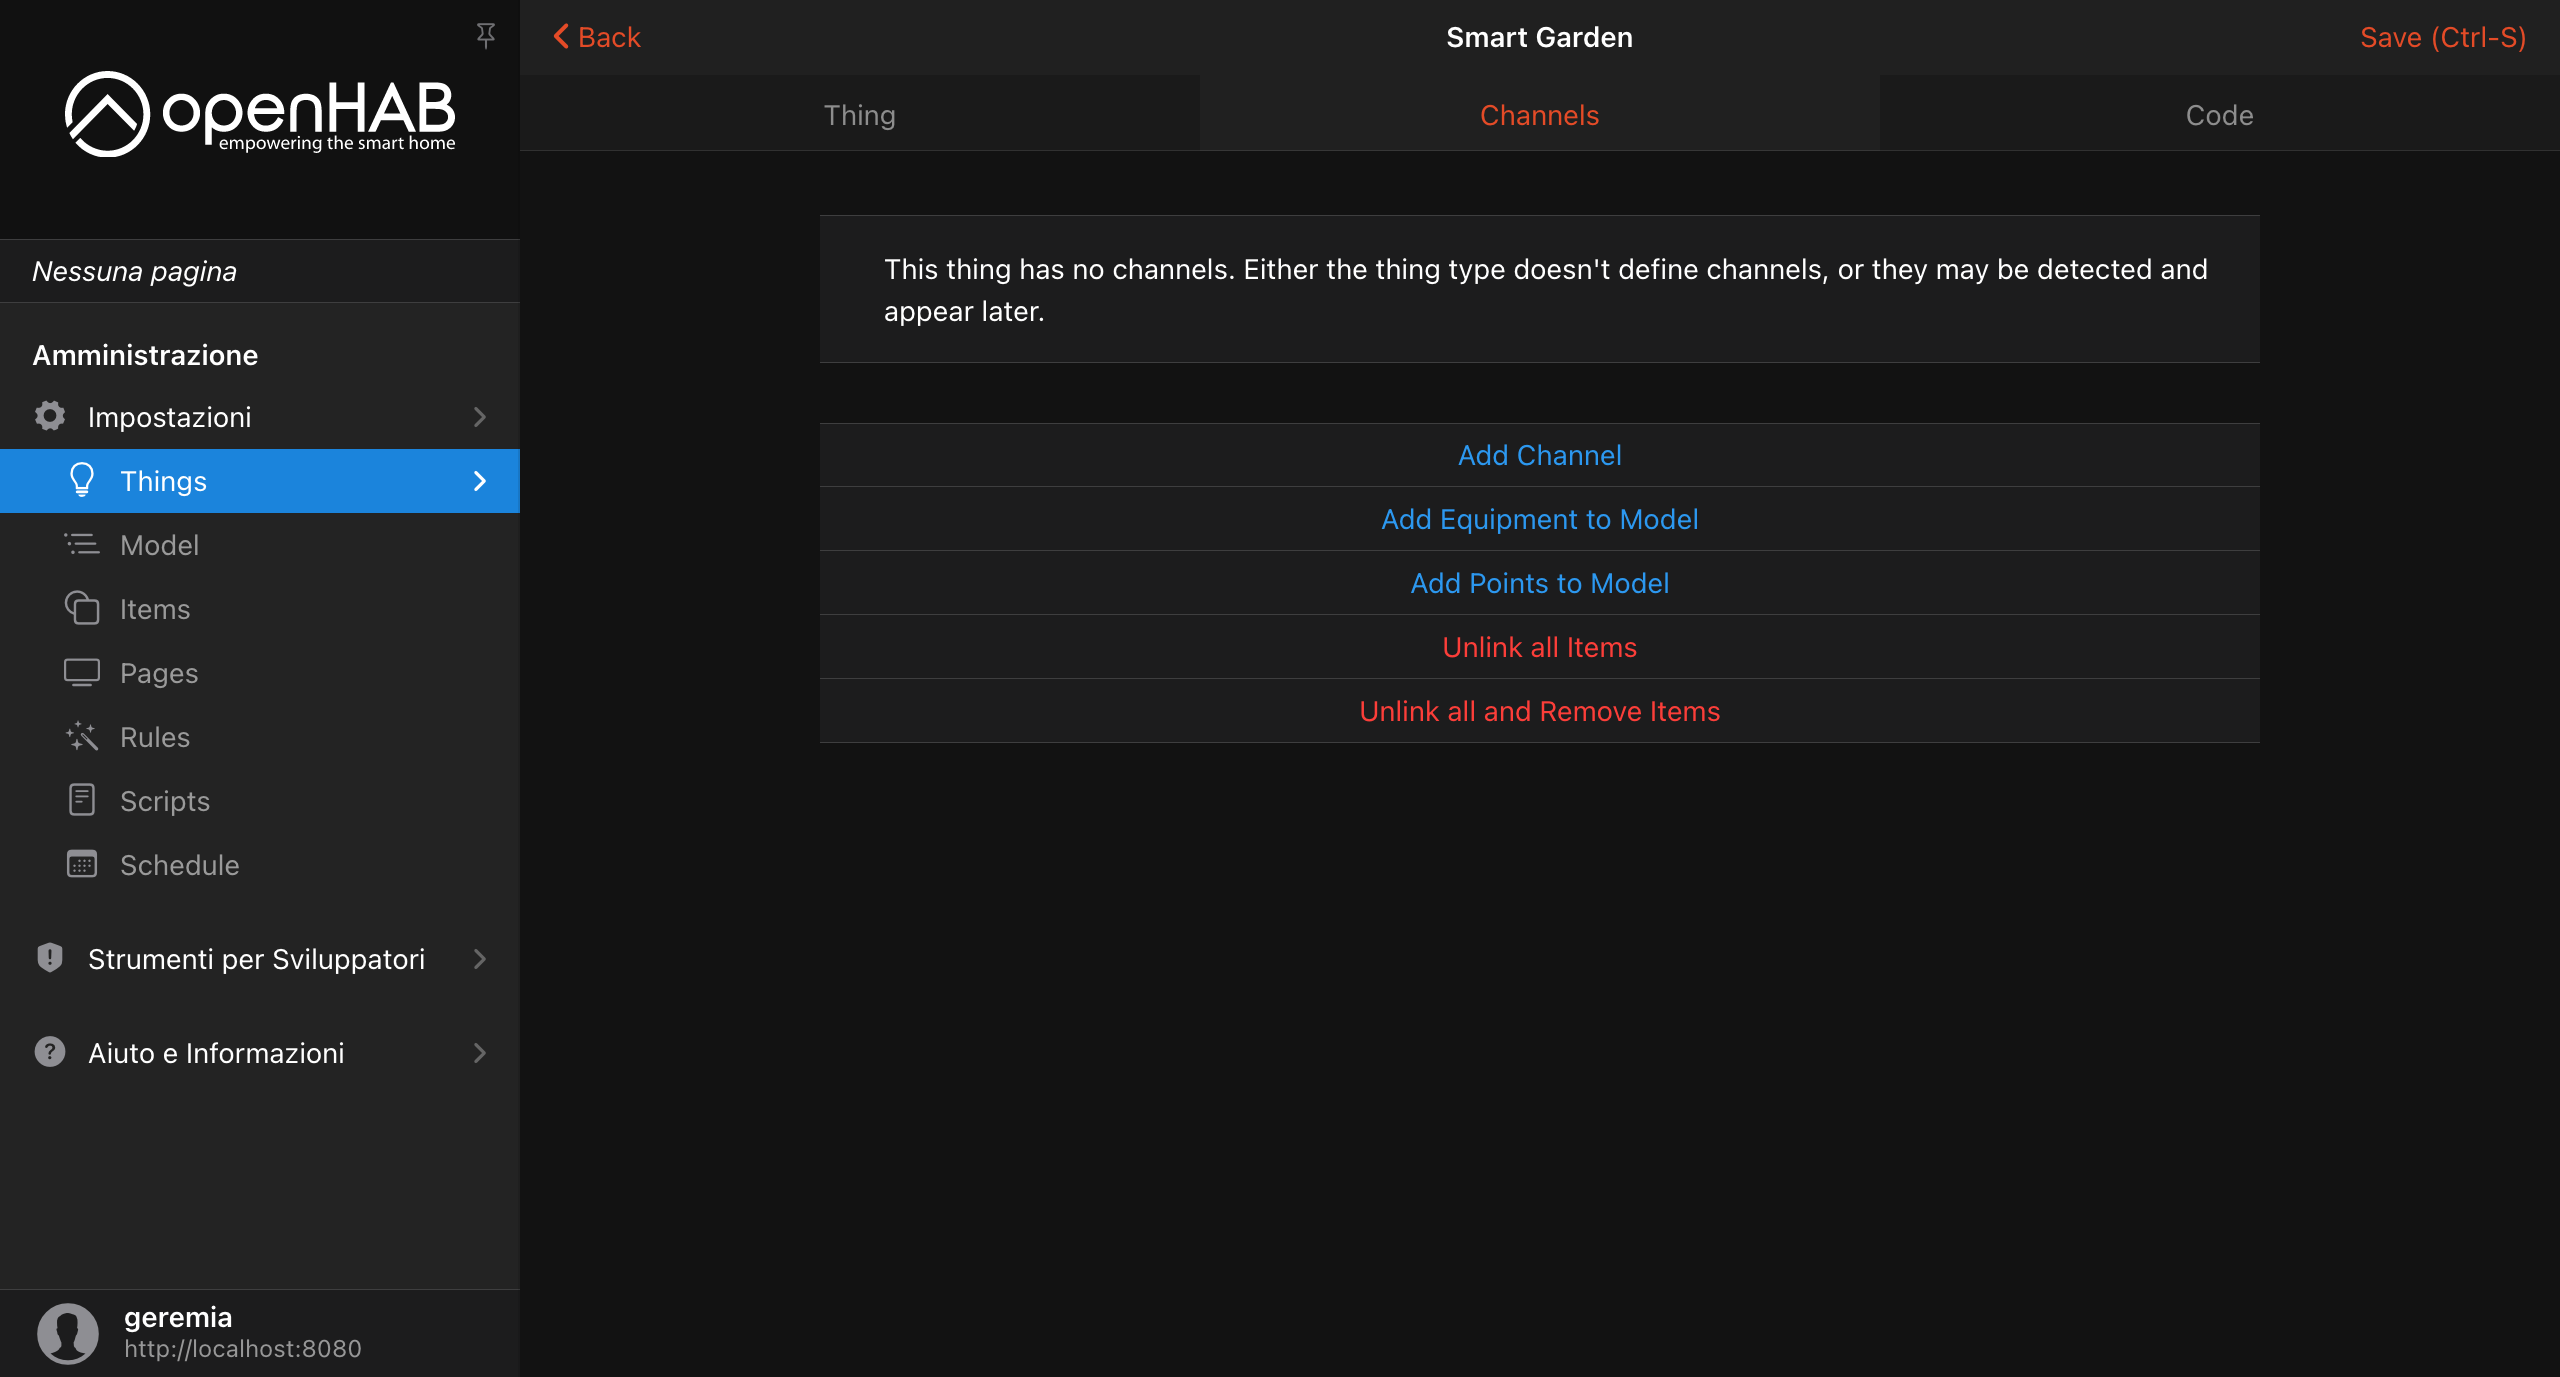
\includegraphics[width=12cm]{Immagini/channels}
        \caption{Schermata Channels}
        \label{fig:channels}
    \end{figure}
    \begin{figure}
        \centering
        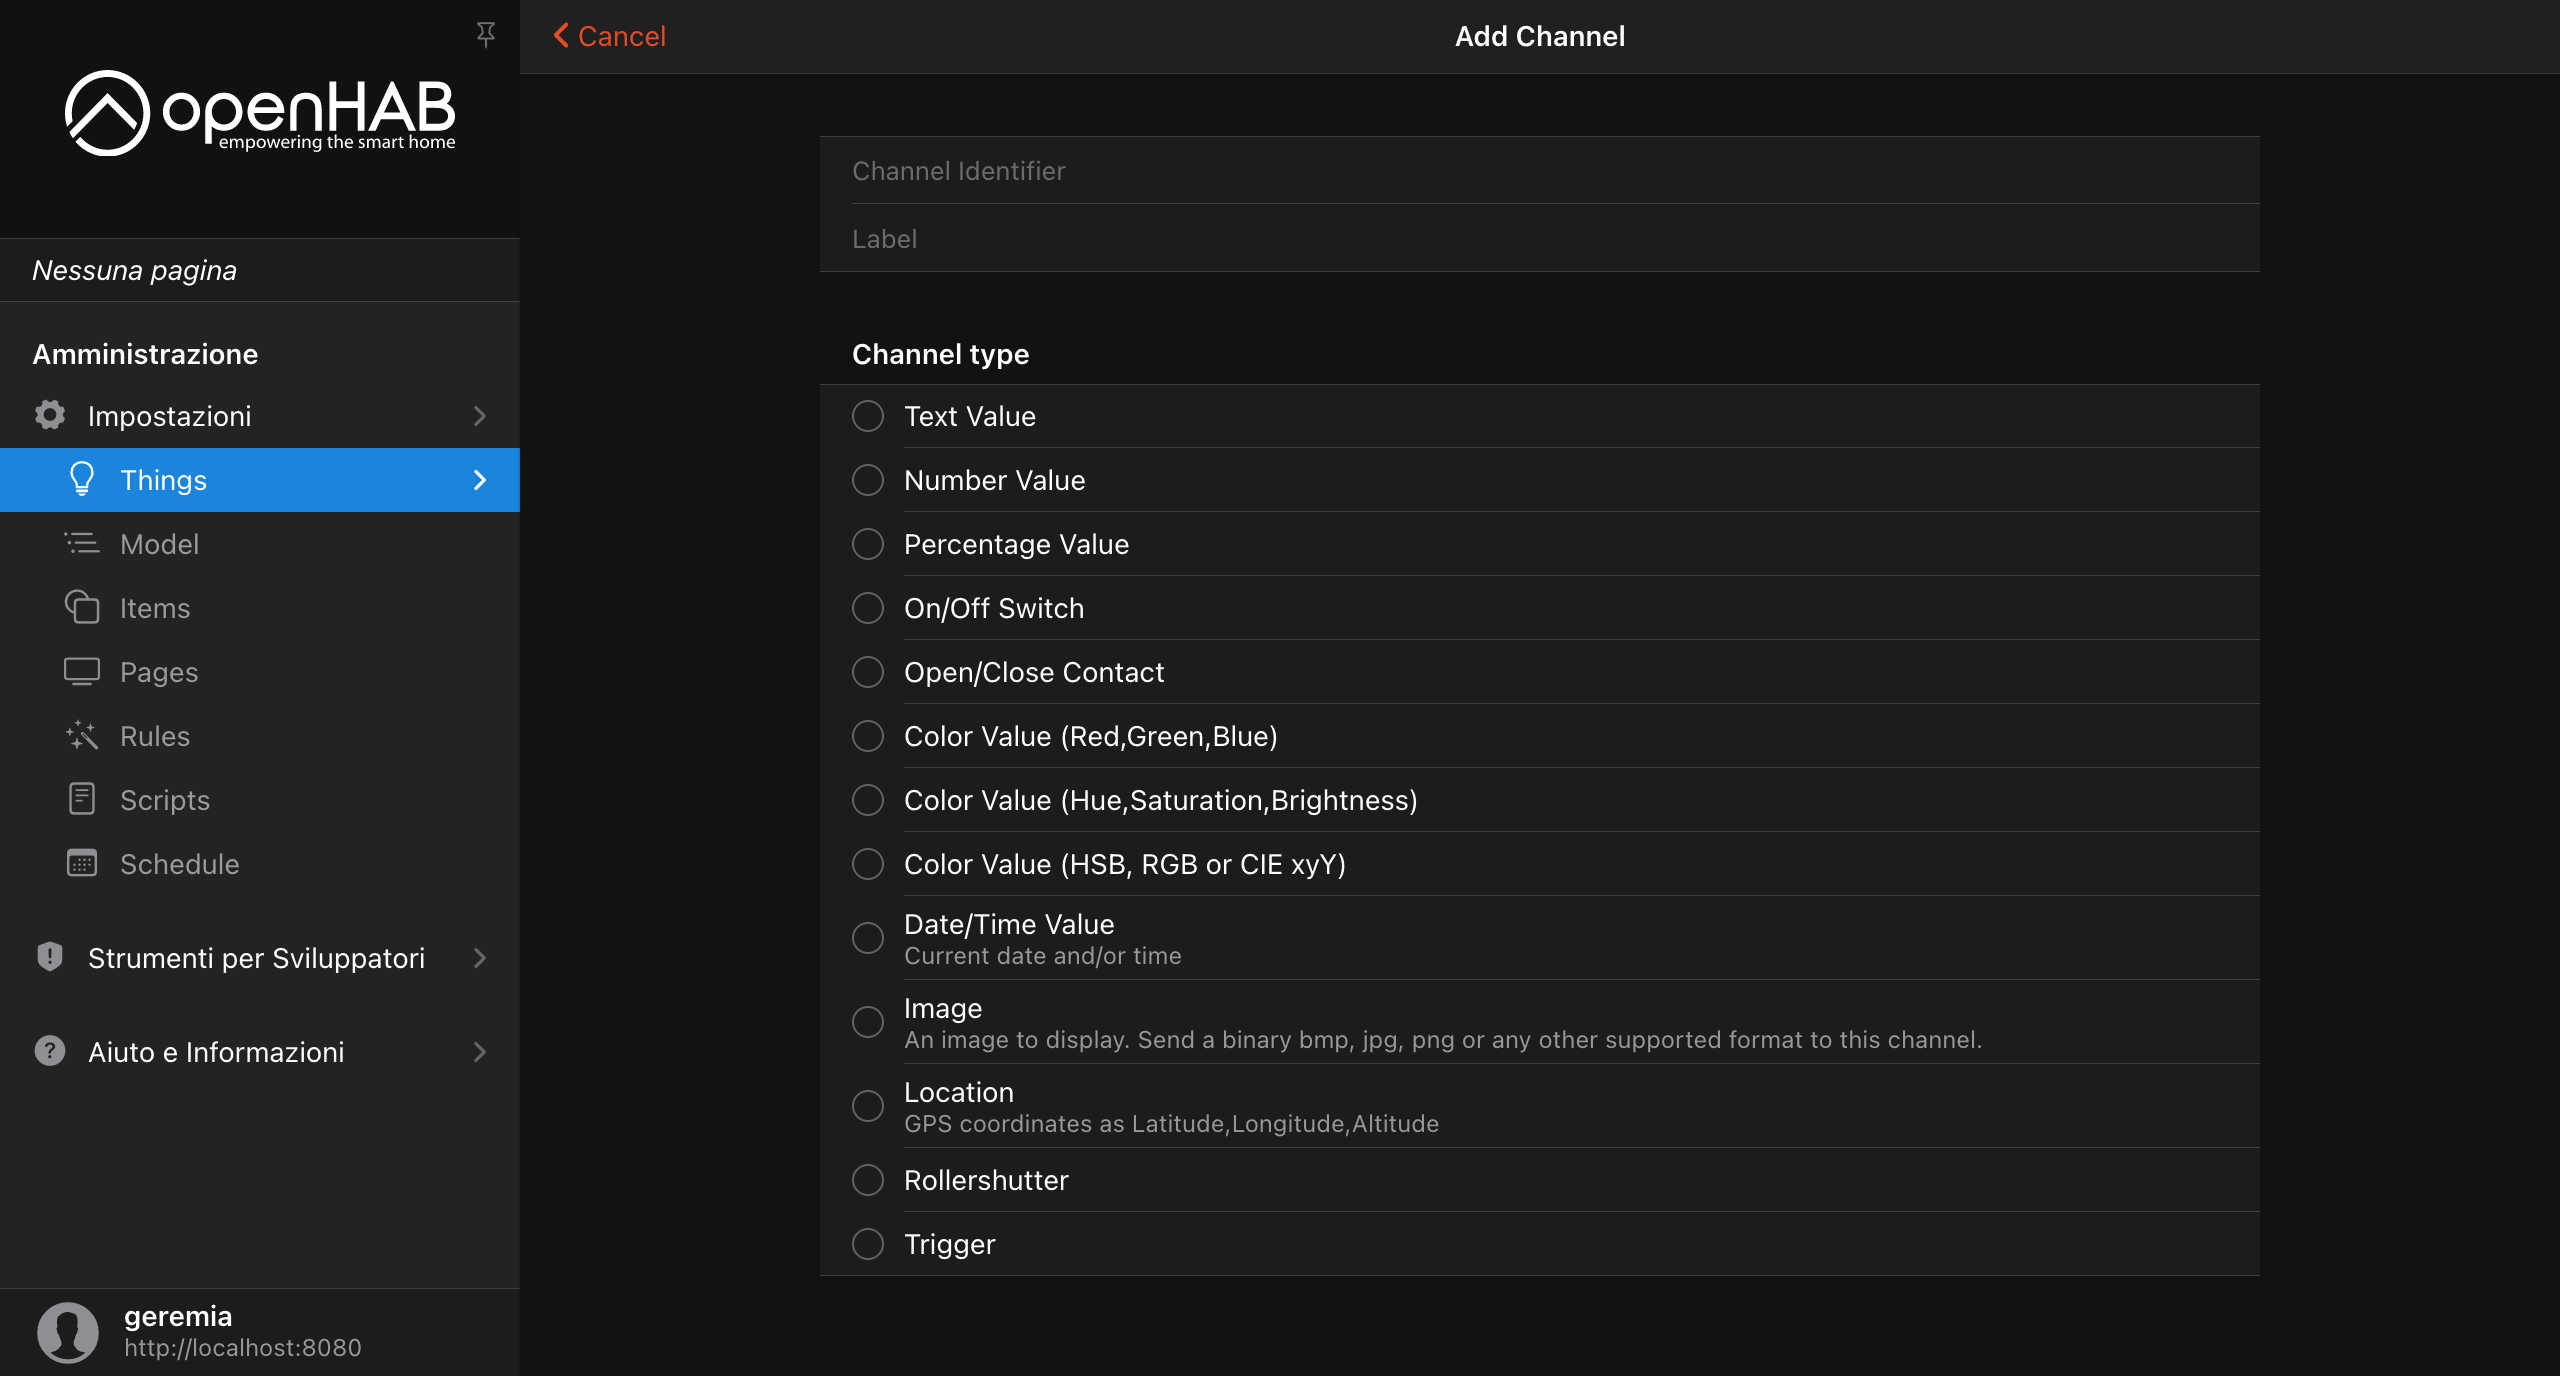
\includegraphics[width=12cm]{Immagini/add_channel}
        \caption{Schermata Add Channel}
        \label{fig:add_channel}
    \end{figure}
    \item successivamente per ogni channels dovrebbe essere creato un item. Per fare ci\'o basta selezionare il channel e premere ``Add Link to Item...''. Dalla schermata Channels quindi si passer\'a poi a quella ``Link Channel to Item'' in cui bisogna selezionare la voce ``Create new Item''. A questo punto basta selezionare una Category (in questo caso ``garden'') e premere ``Link''. Viene ripetuto tale procedimento per ogni Channel (Figura \ref{fig:link_channel_to_item})
    \begin{figure}
        \centering
        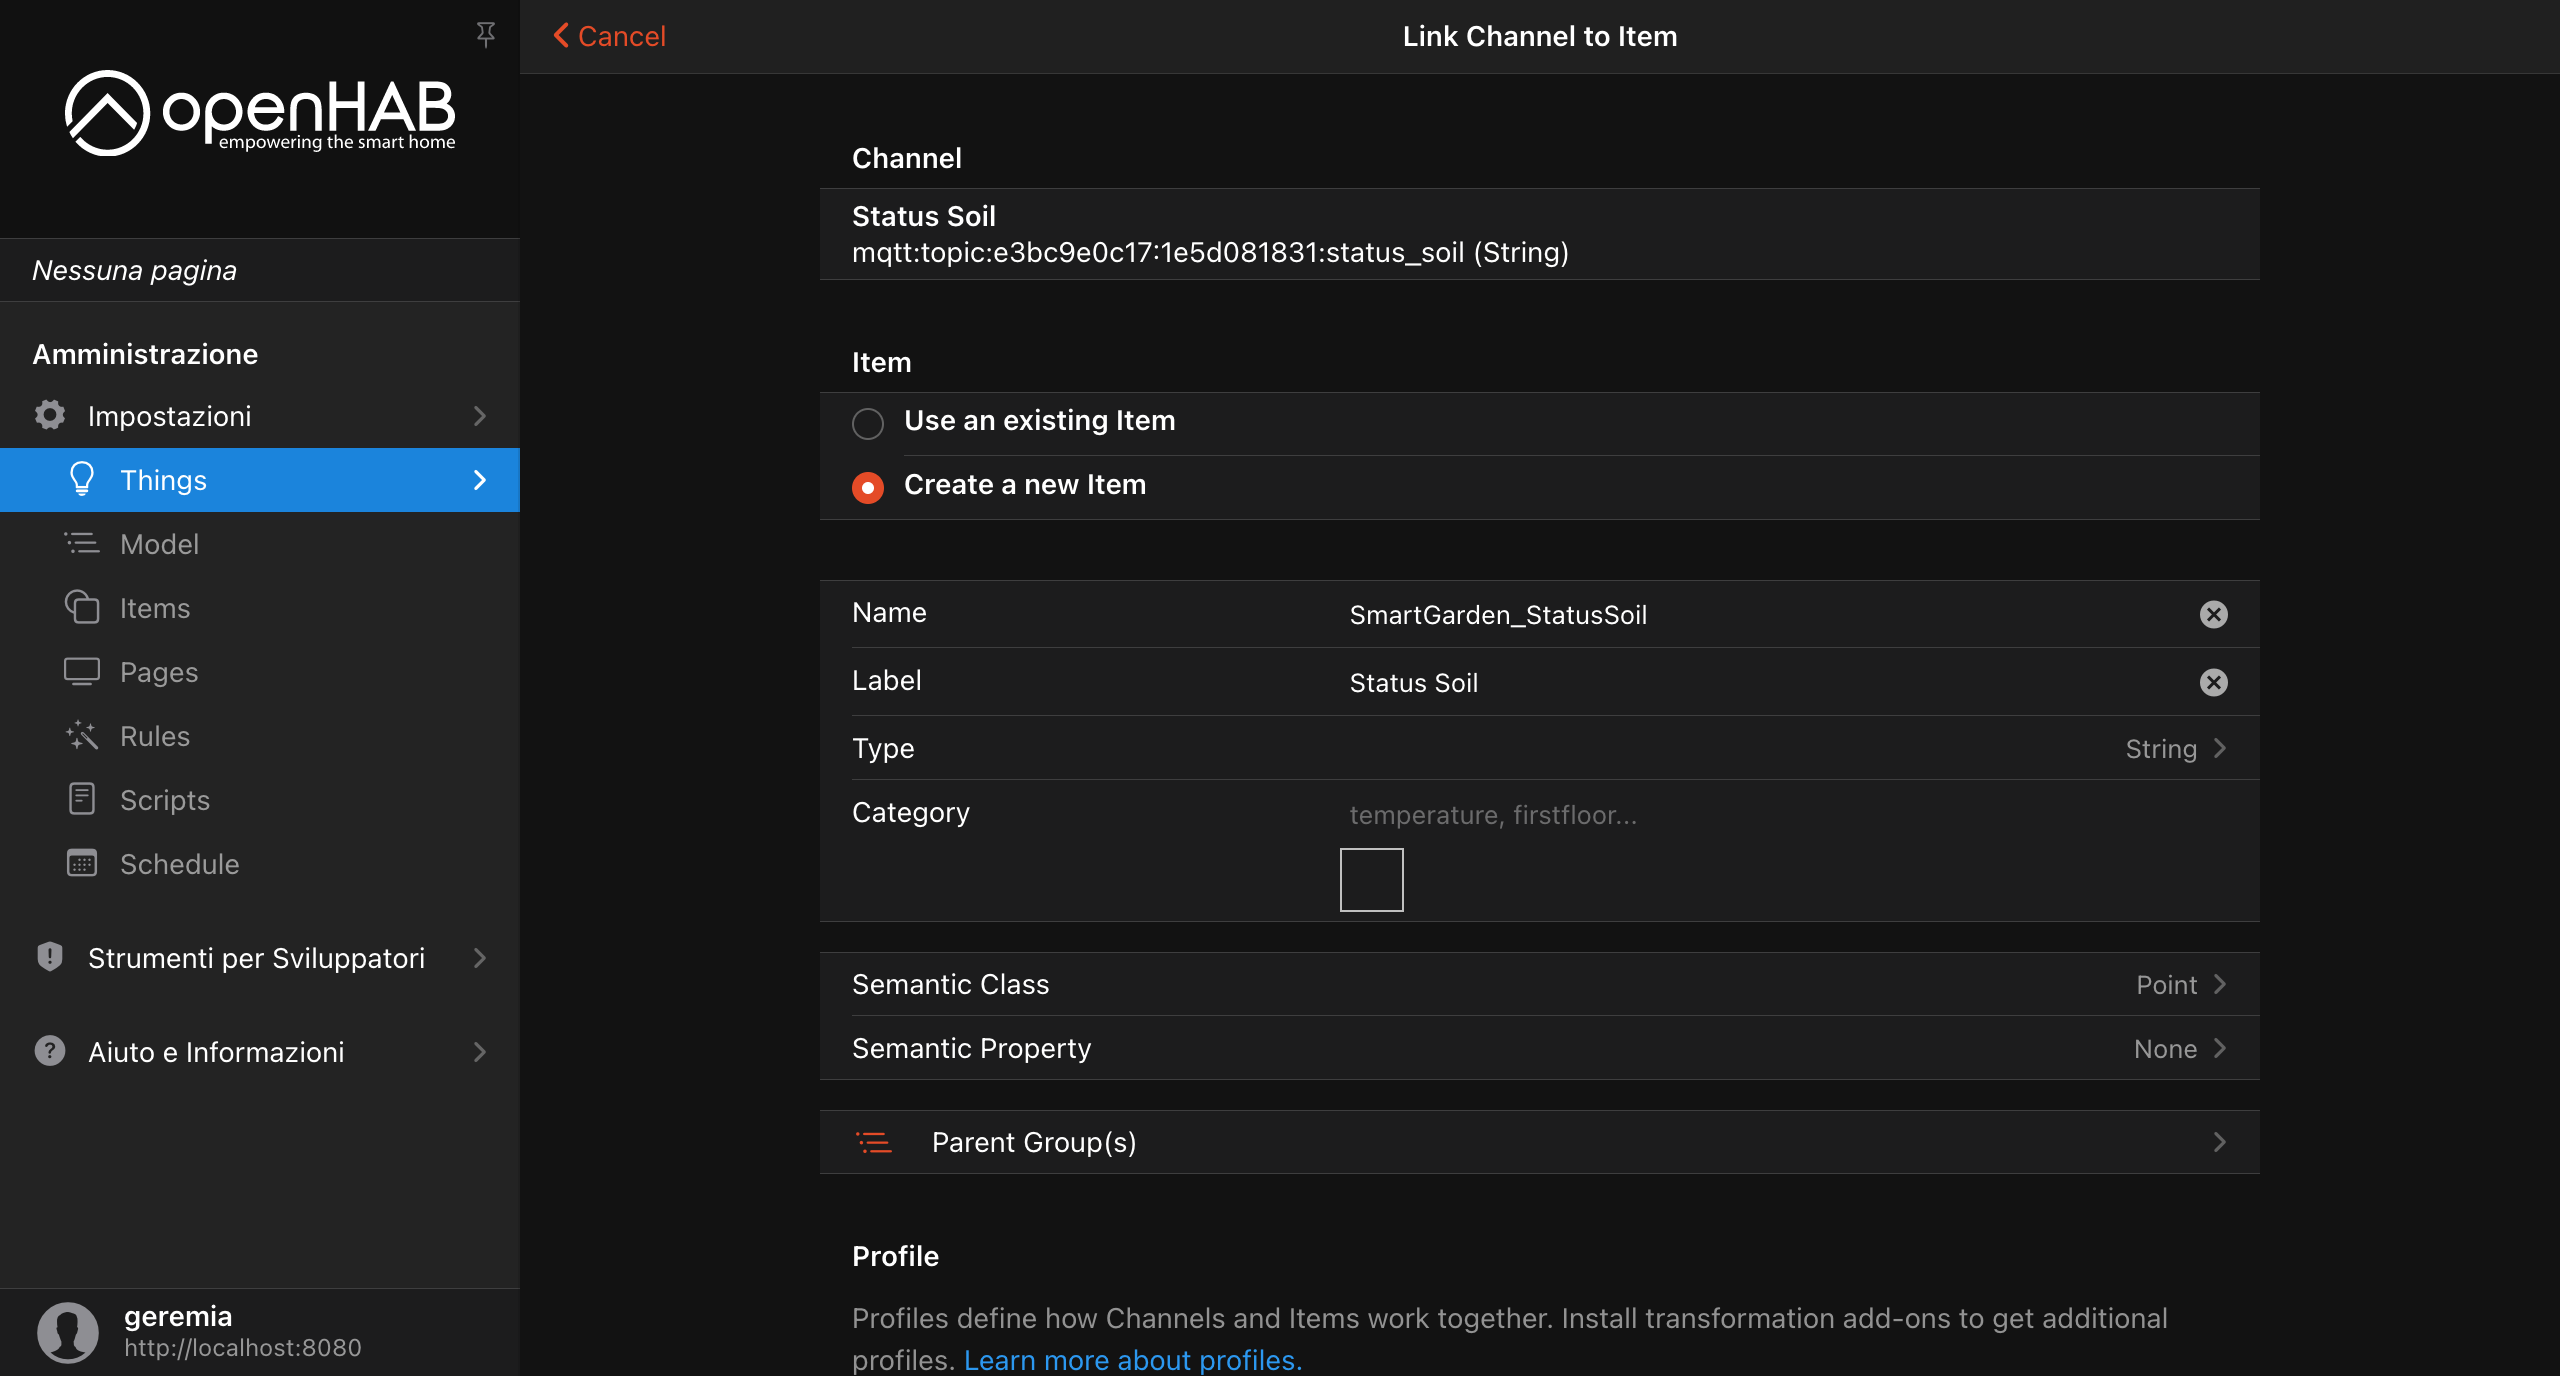
\includegraphics[width=12cm]{Immagini/link_channel_to_item}
        \caption{Schermata Link Channel to Item}
        \label{fig:link_channel_to_item}
    \end{figure}
\end{enumerate}
A questo punto se andiamo alla schermata Items sotto la voce Impostazioni del menu principale possiamo vedere gli Items gi\'a configurati (Figura \ref{fig:configured_items}). Se entriamo in uno di essi \'e possibile sia visualizzare lo stato che, in caso di items collegati a channels dinamici come lo Switch, eseguire un azione per cambiarlo.

\begin{figure}
    \centering
    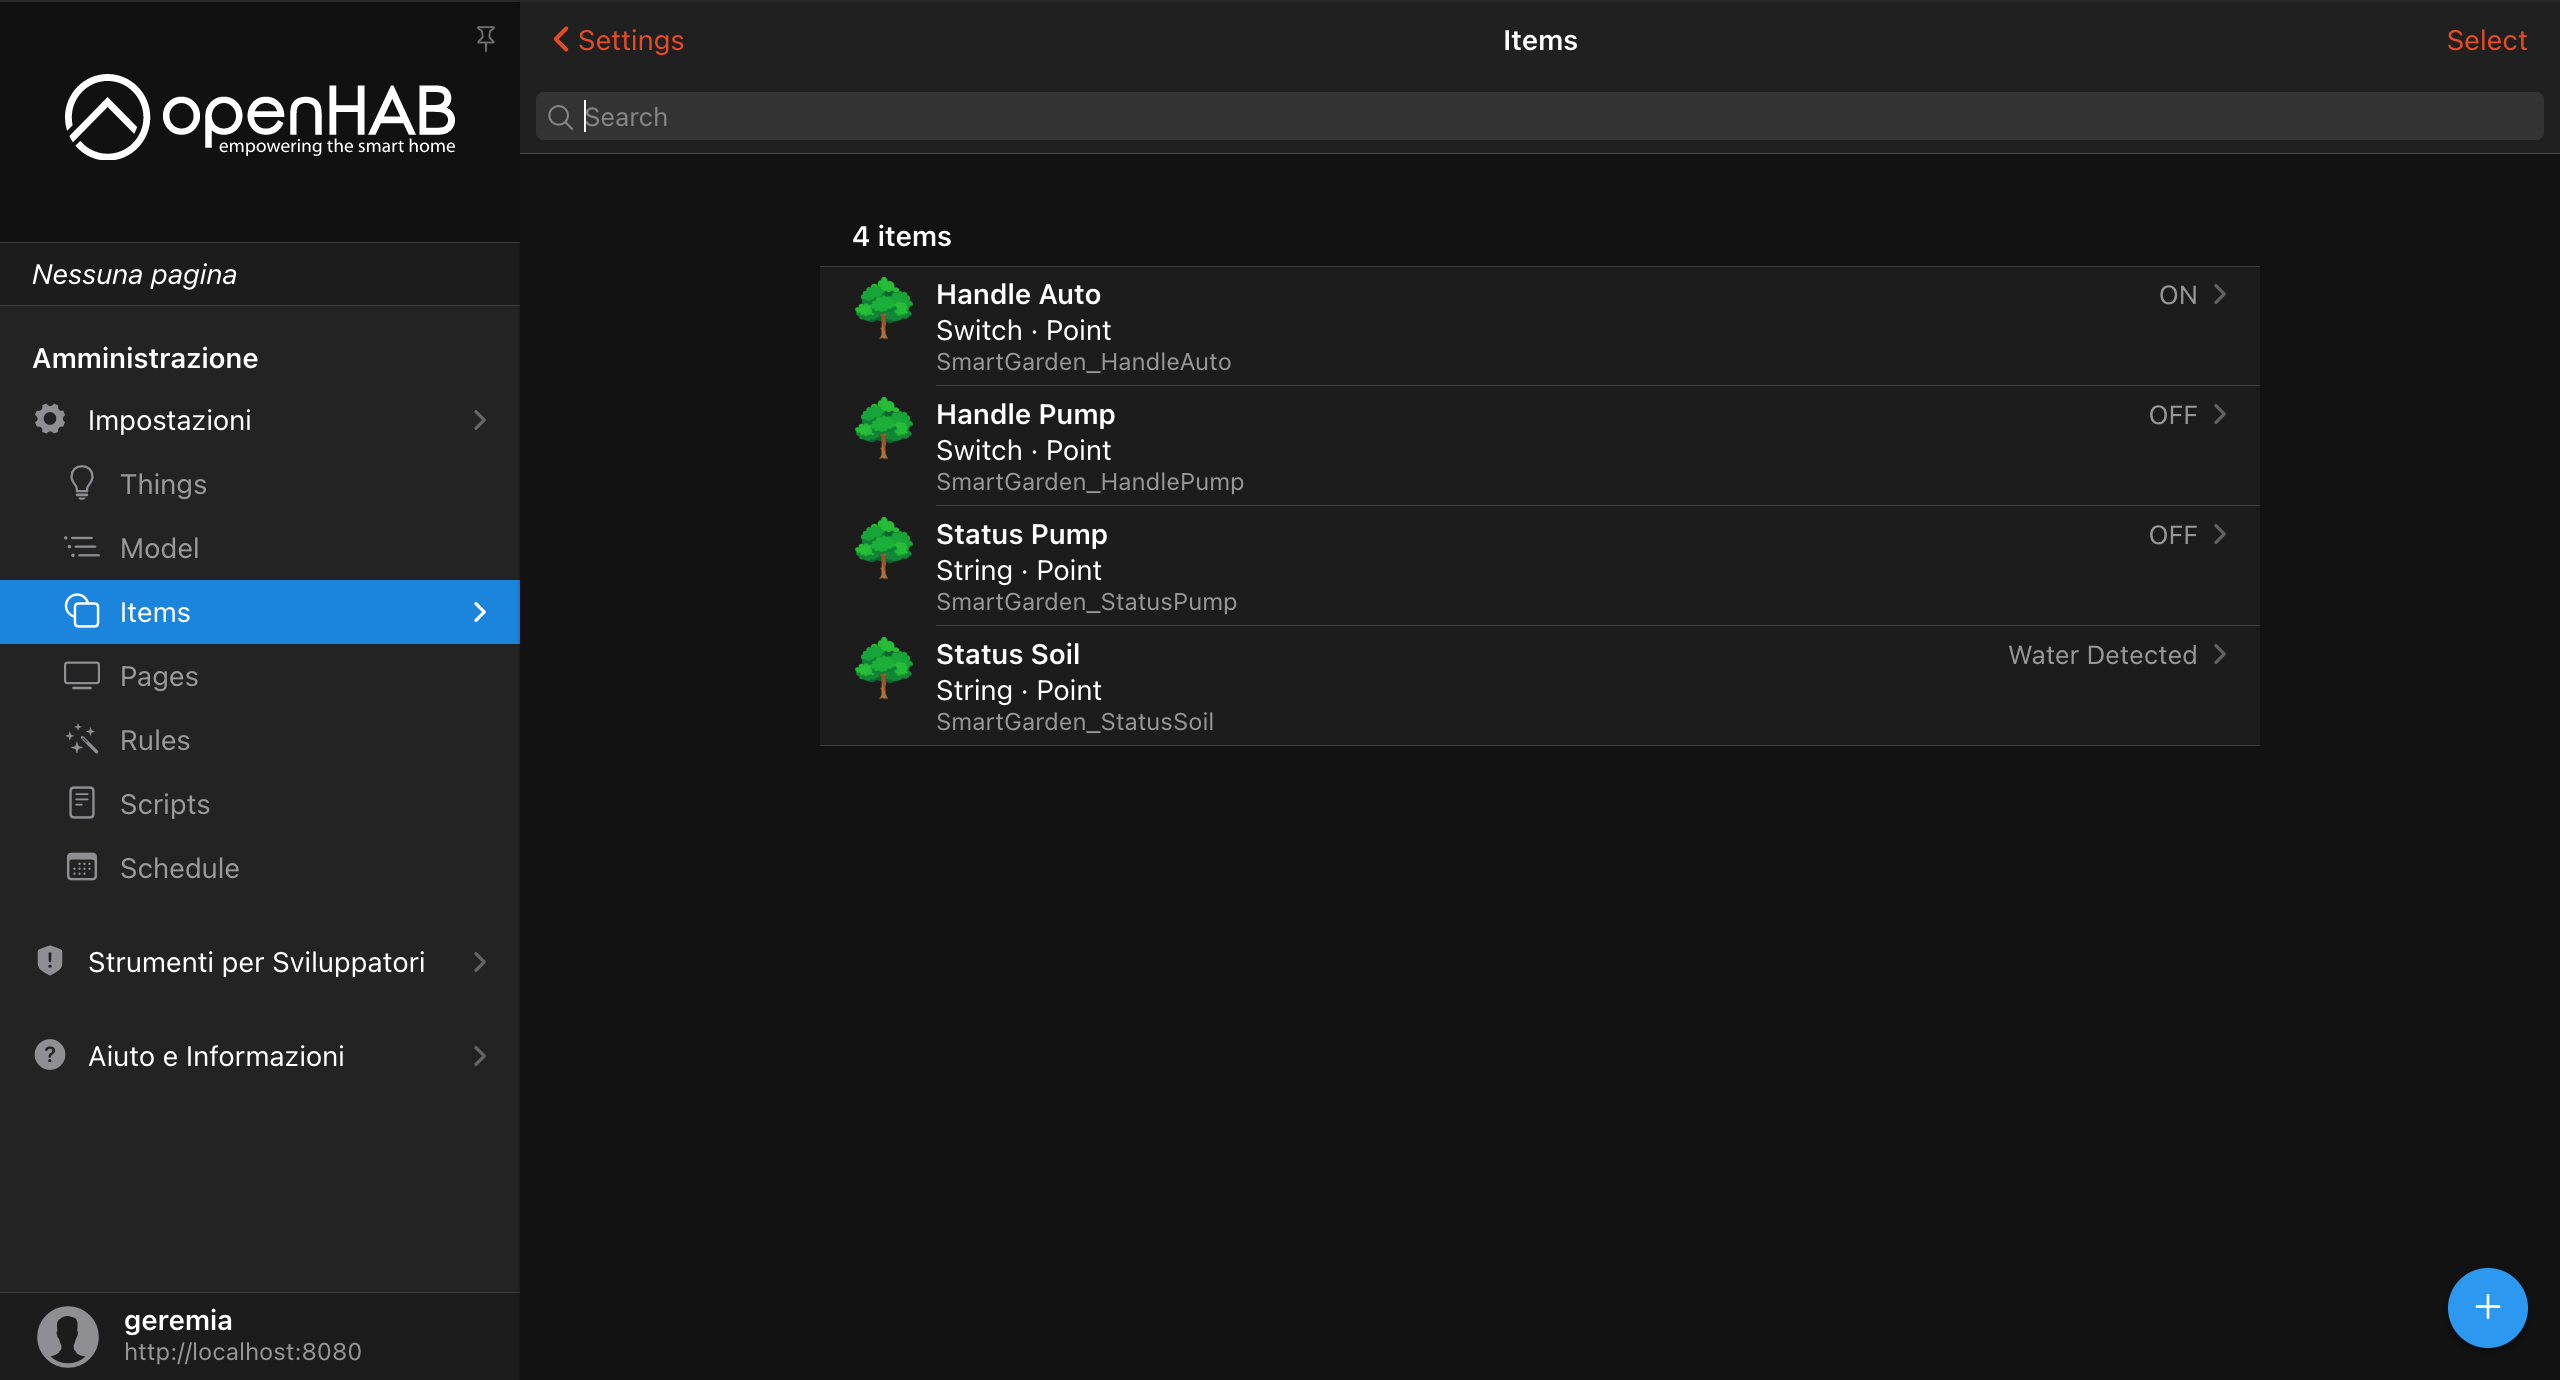
\includegraphics[width=12cm]{Immagini/configured_items}
    \caption{Items Configurati}
    \label{fig:configured_items}
\end{figure}

\subsection{Creazione Sitemap}
Per rendere il tutto pi\'u agevole e user friendly \'e possibile riportare tutto in una Sitemap. Per fare ci\'o bisogna agire all'interno della cartella ``config'' interna a sua volta alla folder principale del software openHAB. In questa cartella \'e possibile aggiungere i vari elementi di openHAB come items e things manualmente tramite file. A questo punto bisogna creare un file all'interno della cartella ``sitemaps'' nominato ``default.sitemap''. Questo \'e il file della Sitemap che andremo a creare. Il codice da scrivere all'interno sar\'a relativo agli Items aggiunti, infatti essi possono essere aggiunti tramite il loro identificativo che si trova nella propria schermata in alto. Possono essere aggiunte anche icone per rendere pi\'u immediata la schermata. In questo caso facciamo riferimento al Codice \ref{code:sitemap_smart_garden_code} dove troviamo il Frame ``Garden'' che contiene gli Items impostati precedentemente con relative icone e label (in caso di text value). \'E possibile poi visualizzare l'interfaccia web andando all'url \texttt{http://localhost:8080/basicui/app}. \'E possibile inoltre controllare ci\'o tramite smartphone installando l'applicazione di openHAB e configurandola aggiungendo indirizzo ip e porta del server openHAB interno alla propria rete locale (Figure \ref{fig:sitemap_smart_garden_ui_web} e \ref{fig:sitemap_smart_garden_ui_app}).

\begin{lstlisting}[caption=Sitemap Smart Garden Code,label=code:sitemap_smart_garden_code]
sitemap default label="Home"
{
    Frame label="Garden" 
    {
        Switch item=SmartGarden_HandlePump icon="switch"
        Switch item=SmartGarden_HandleAuto icon="switch"
        Text item=SmartGarden_StatusPump label="[%s]" icon="pump"
        Text item=SmartGarden_StatusSoil label="[%s]" icon="water"
    }
}
\end{lstlisting}

\begin{figure}
    \centering
    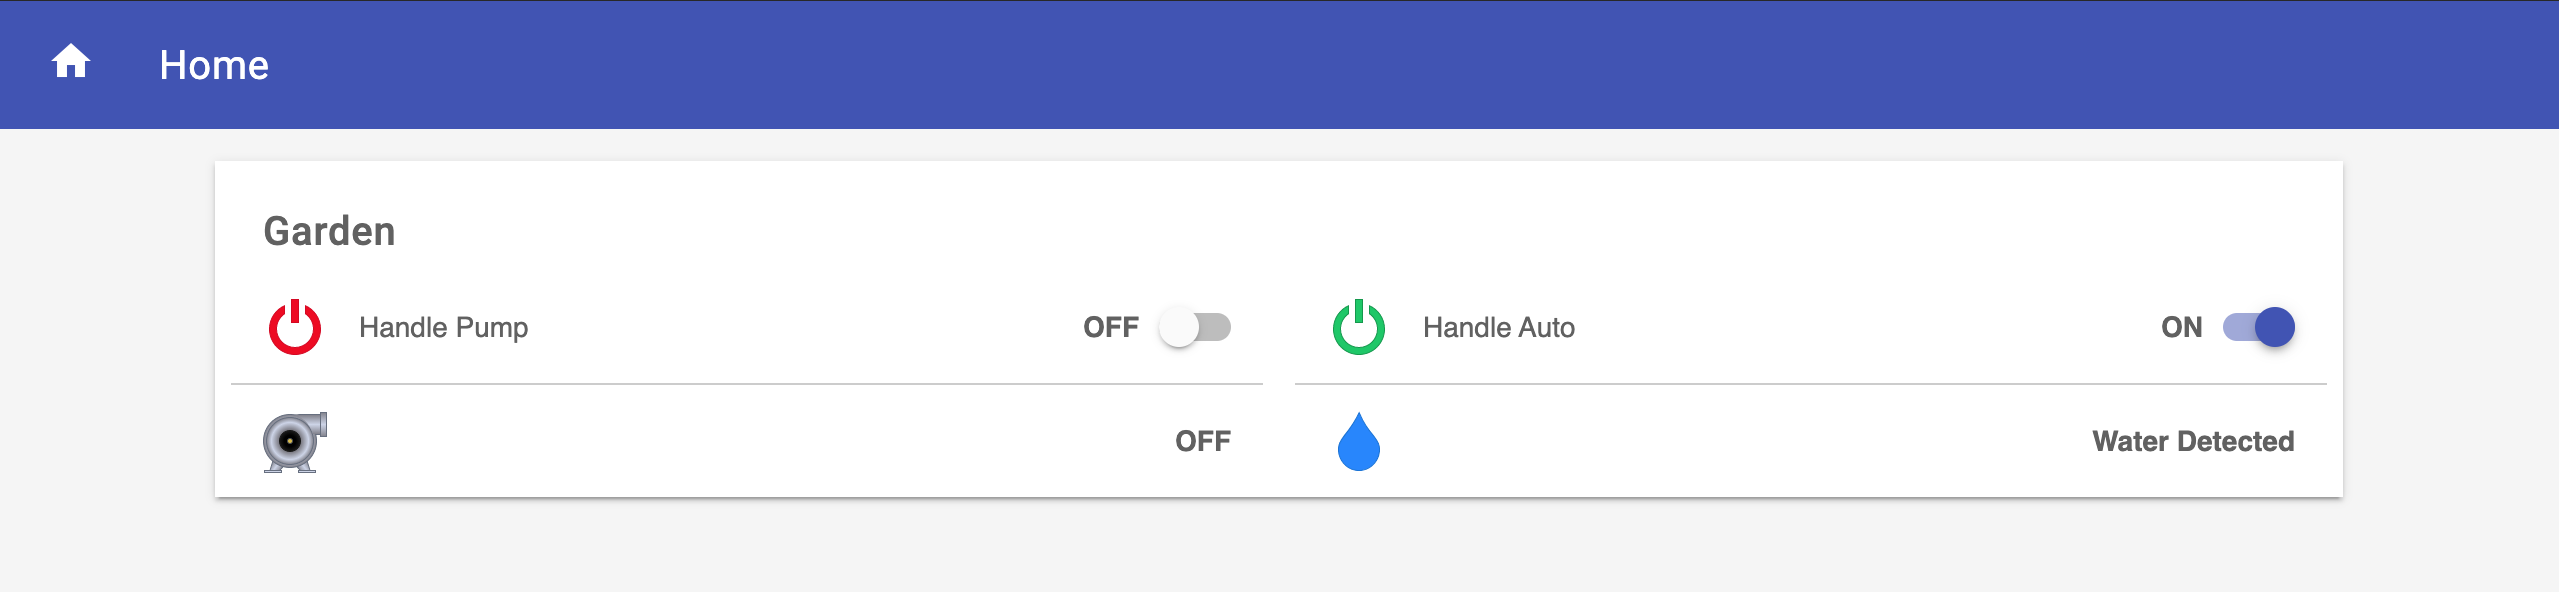
\includegraphics[width=12cm]{Immagini/sitemap_smart_garden_ui_web}
    \caption{Sitemap Smart Garden UI Web}
    \label{fig:sitemap_smart_garden_ui_web}
\end{figure}

\begin{figure}
    \centering
    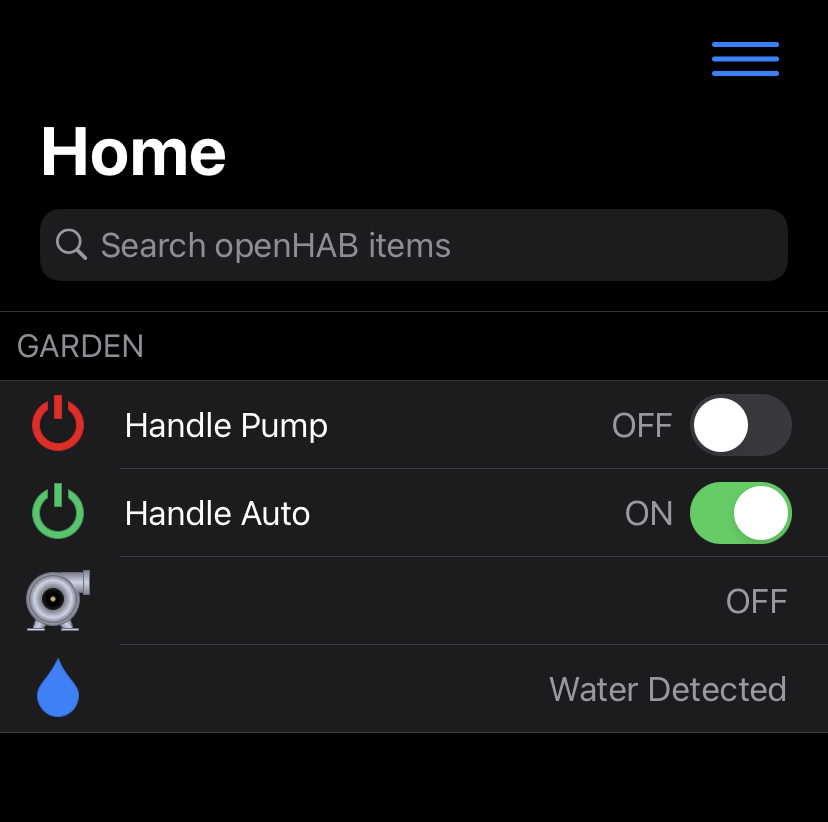
\includegraphics[width=12cm]{Immagini/sitemap_smart_garden_ui_app}
    \caption{Sitemap Smart Garden UI App}
    \label{fig:sitemap_smart_garden_ui_app}
\end{figure}
\chapter{Conclusioni}
Arrivati a questo punto si pu\'o confermare la versatilit\'a di {\em openHAB} al dialogo con qualsiasi tipo di dispositivo. Con lo sviluppo del sistema IOT e il collegamento di esso al software per la domotica si \'e riuscito a controllare l'irrigazione di un piccolo vaso di basilico. Esso quindi pu\'o essere tranquillamente gestito dal computer o dal proprio smartphone abilitando la modalit\'a automatica o accendendo e spegnendo manualmente la pompa dell'acqua. Inoltre \'e possibile anche visualizzare i vari stati relativi al sensore di umidit\'a e alla pompa dell'acqua. Possono essere visualizzati i risultati del lavoro alle Figure \ref{fig:smart_garden_1}, \ref{fig:smart_garden_2}, \ref{fig:smart_garden_3}, \ref{fig:smart_garden_4}.

\begin{figure}
    \centering
    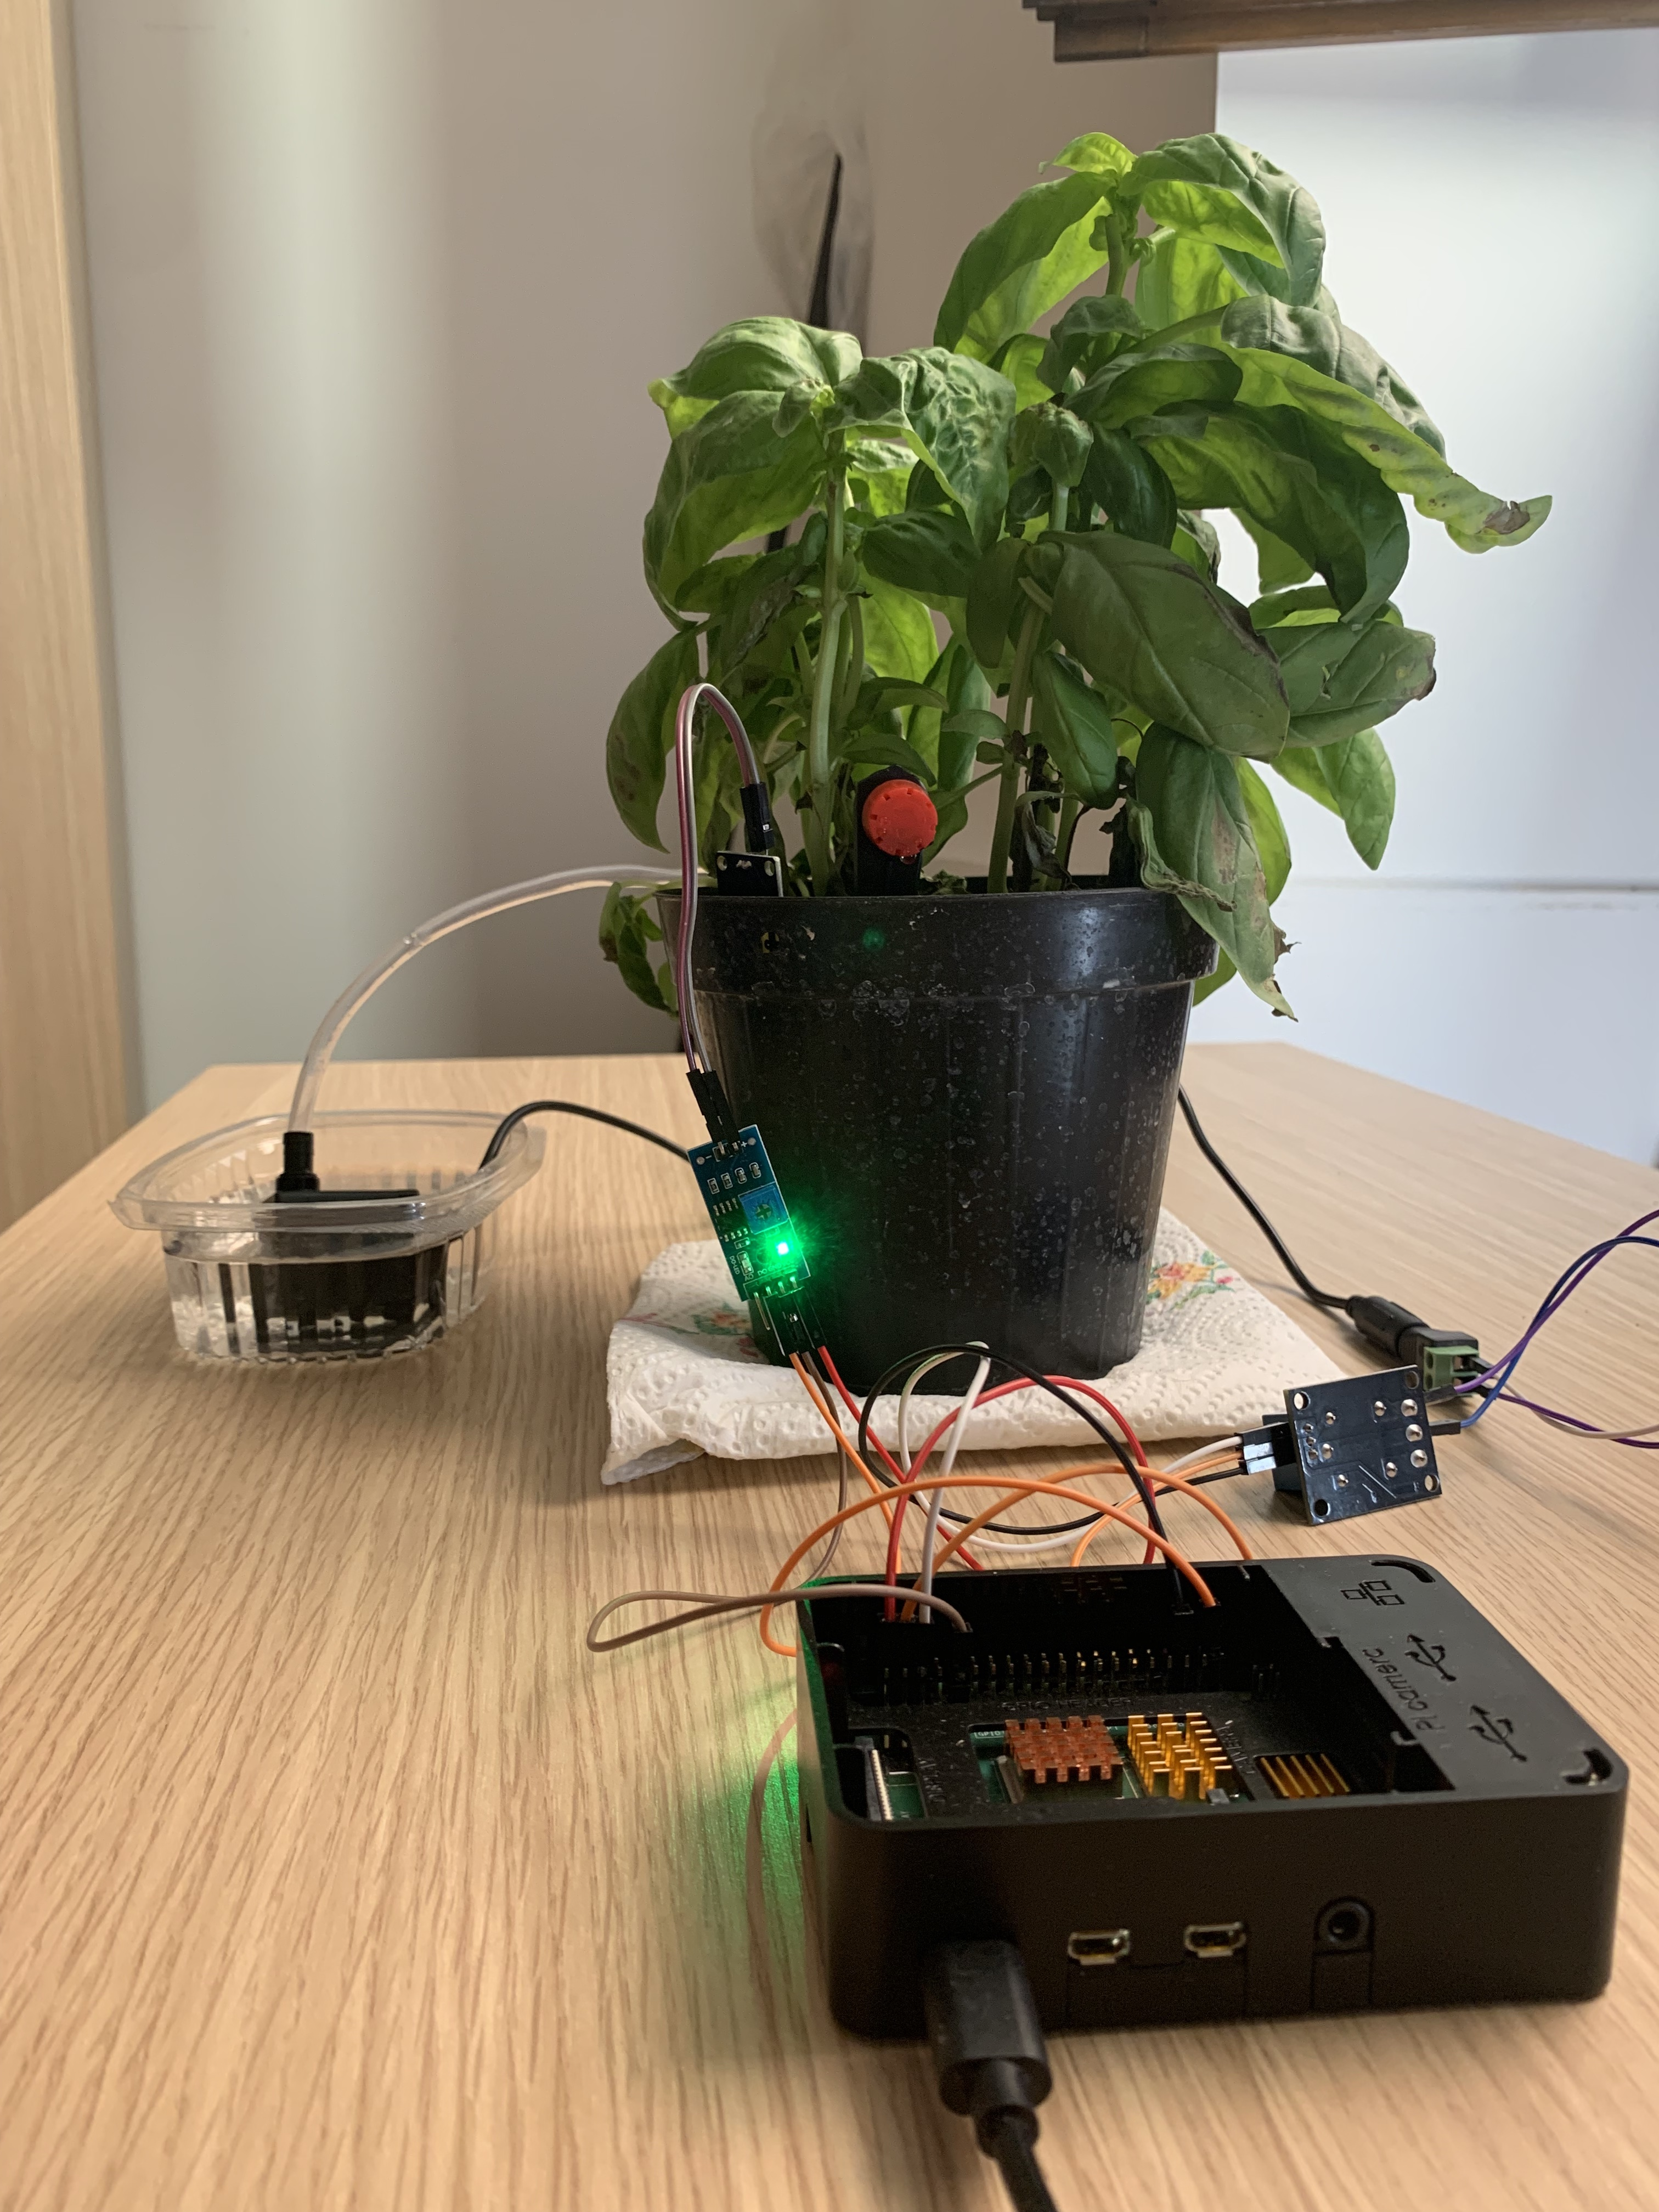
\includegraphics[width=12cm]{Immagini/smart_garden_1}
    \caption{Smart Garden di fianco}
    \label{fig:smart_garden_1}
\end{figure}

\begin{figure}
    \centering
    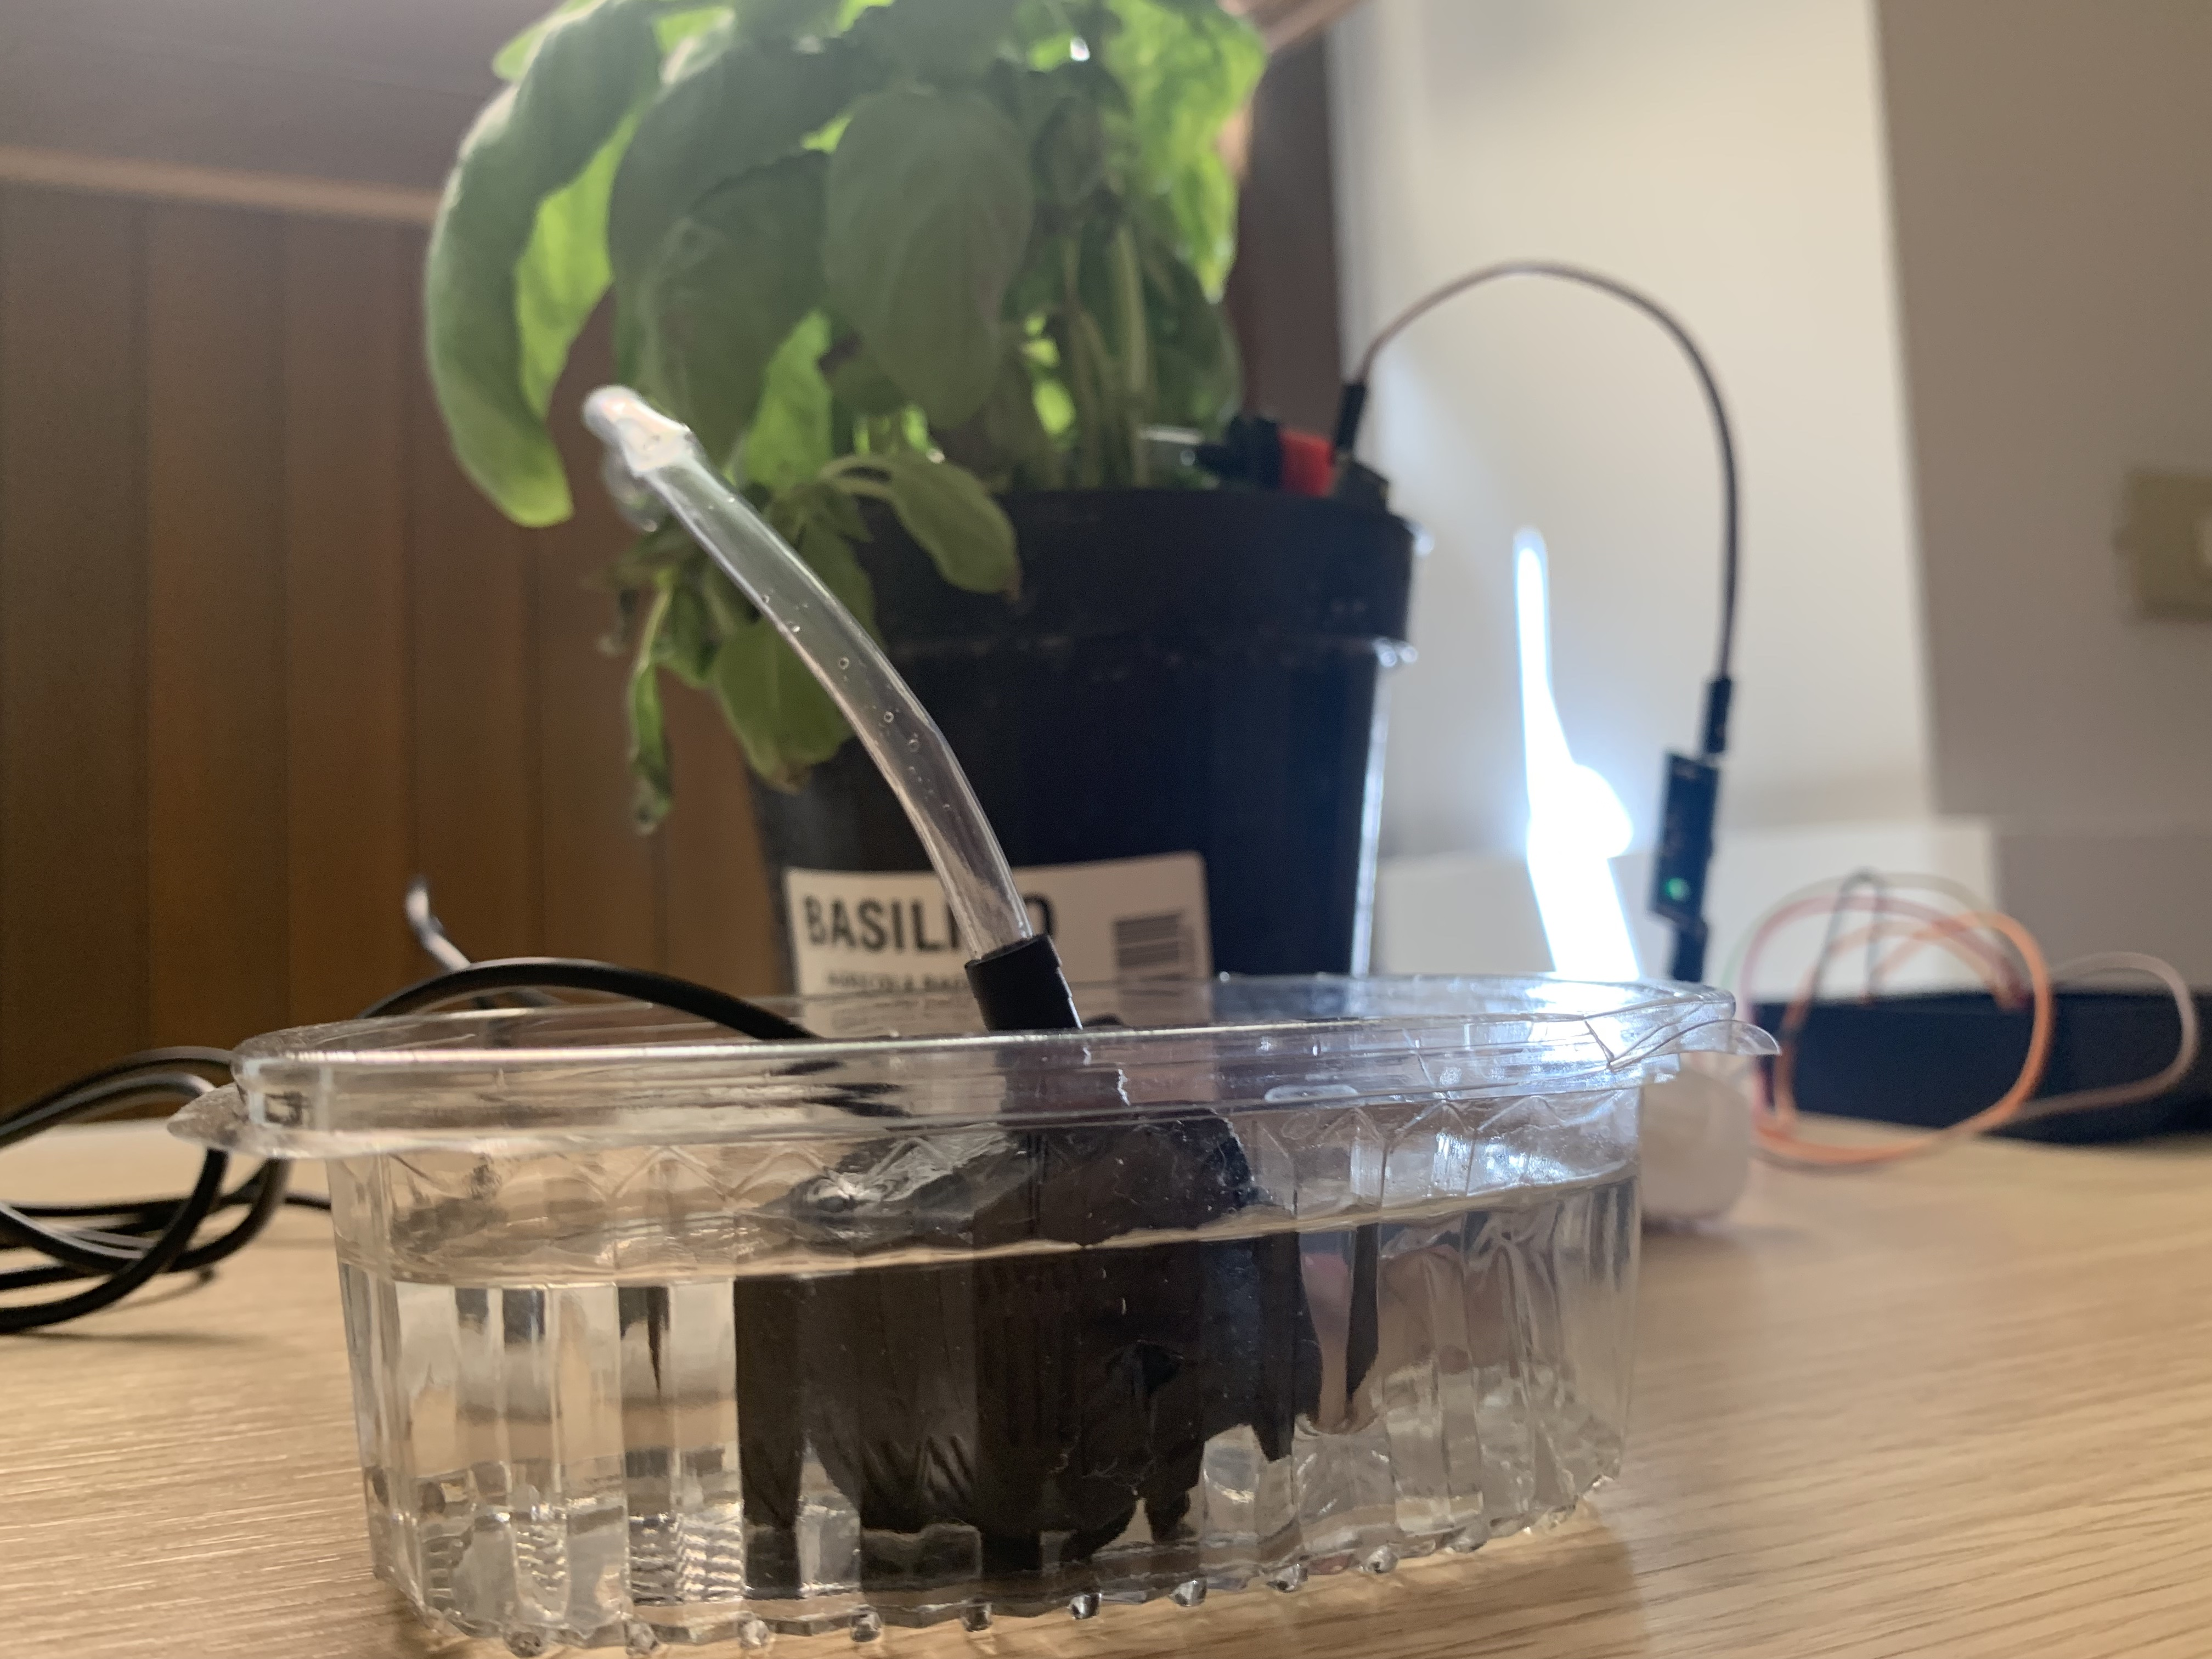
\includegraphics[width=12cm]{Immagini/smart_garden_2}
    \caption{Smart Garden pompa dell'acqua}
    \label{fig:smart_garden_2}
\end{figure}

\begin{figure}
    \centering
    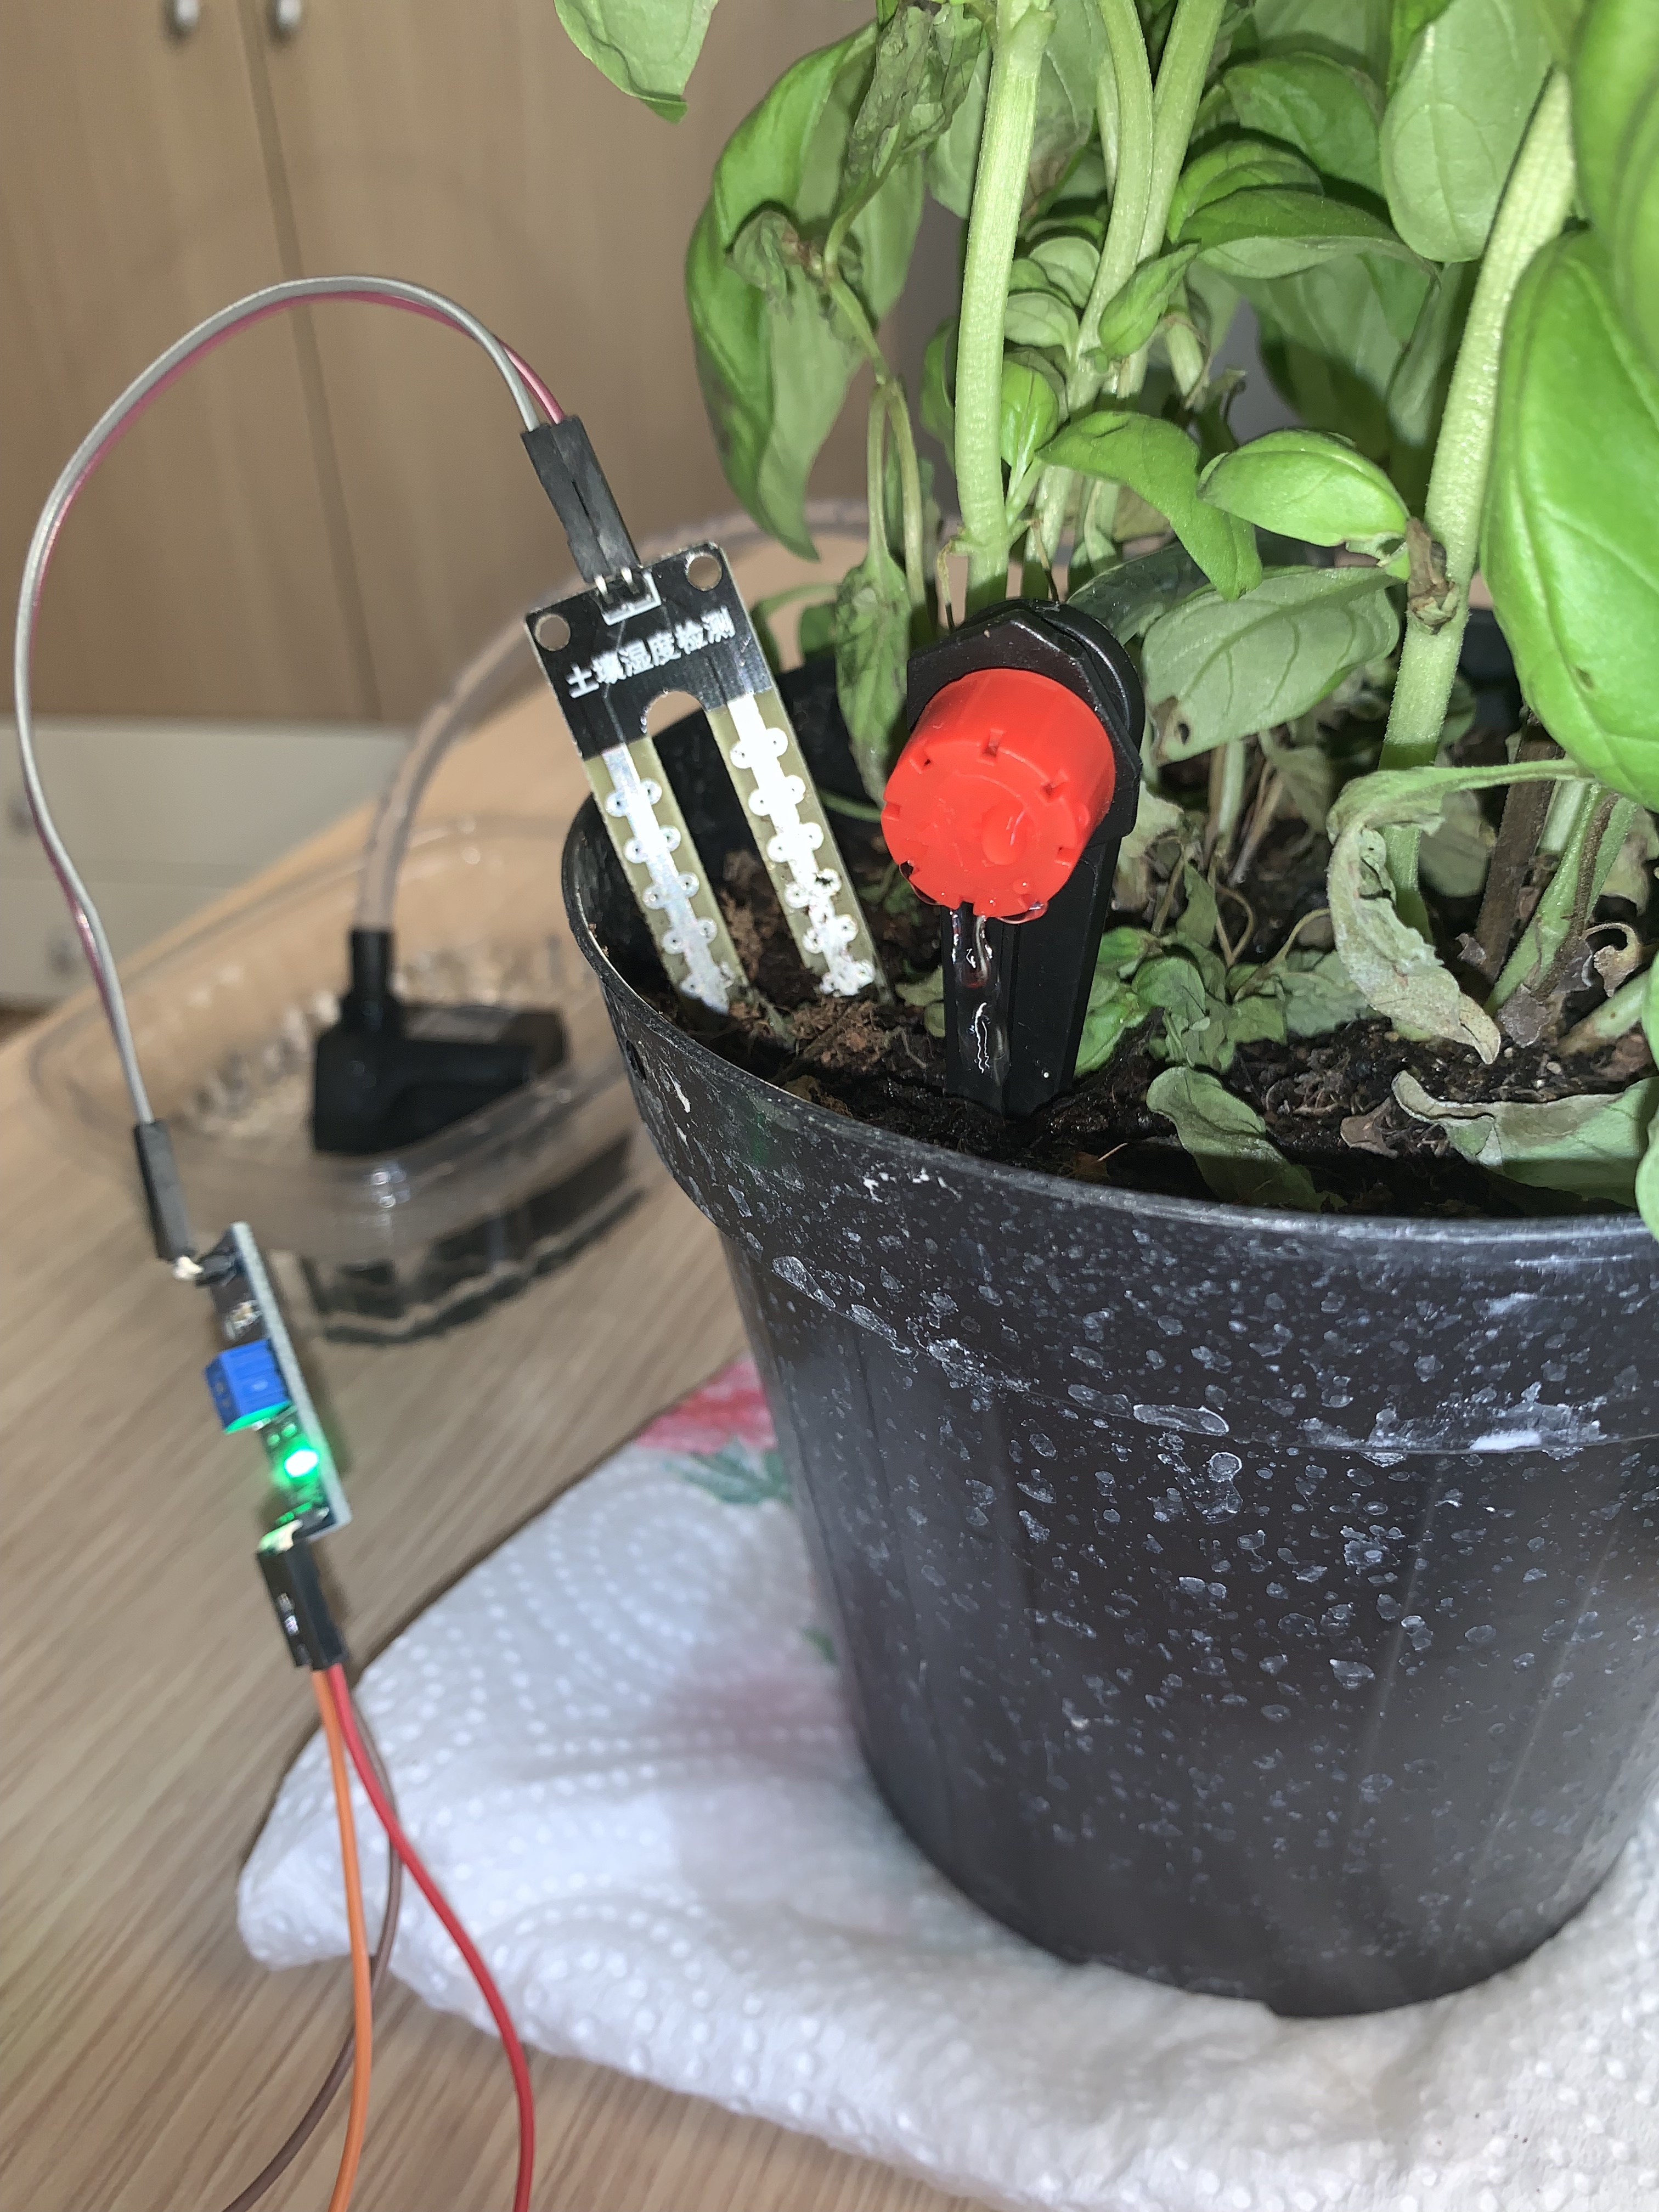
\includegraphics[width=12cm]{Immagini/smart_garden_3}
    \caption{Smart Garden sensore di umidit\'a e erogazione dell'acqua}
    \label{fig:smart_garden_3}
\end{figure}

\begin{figure}
    \centering
    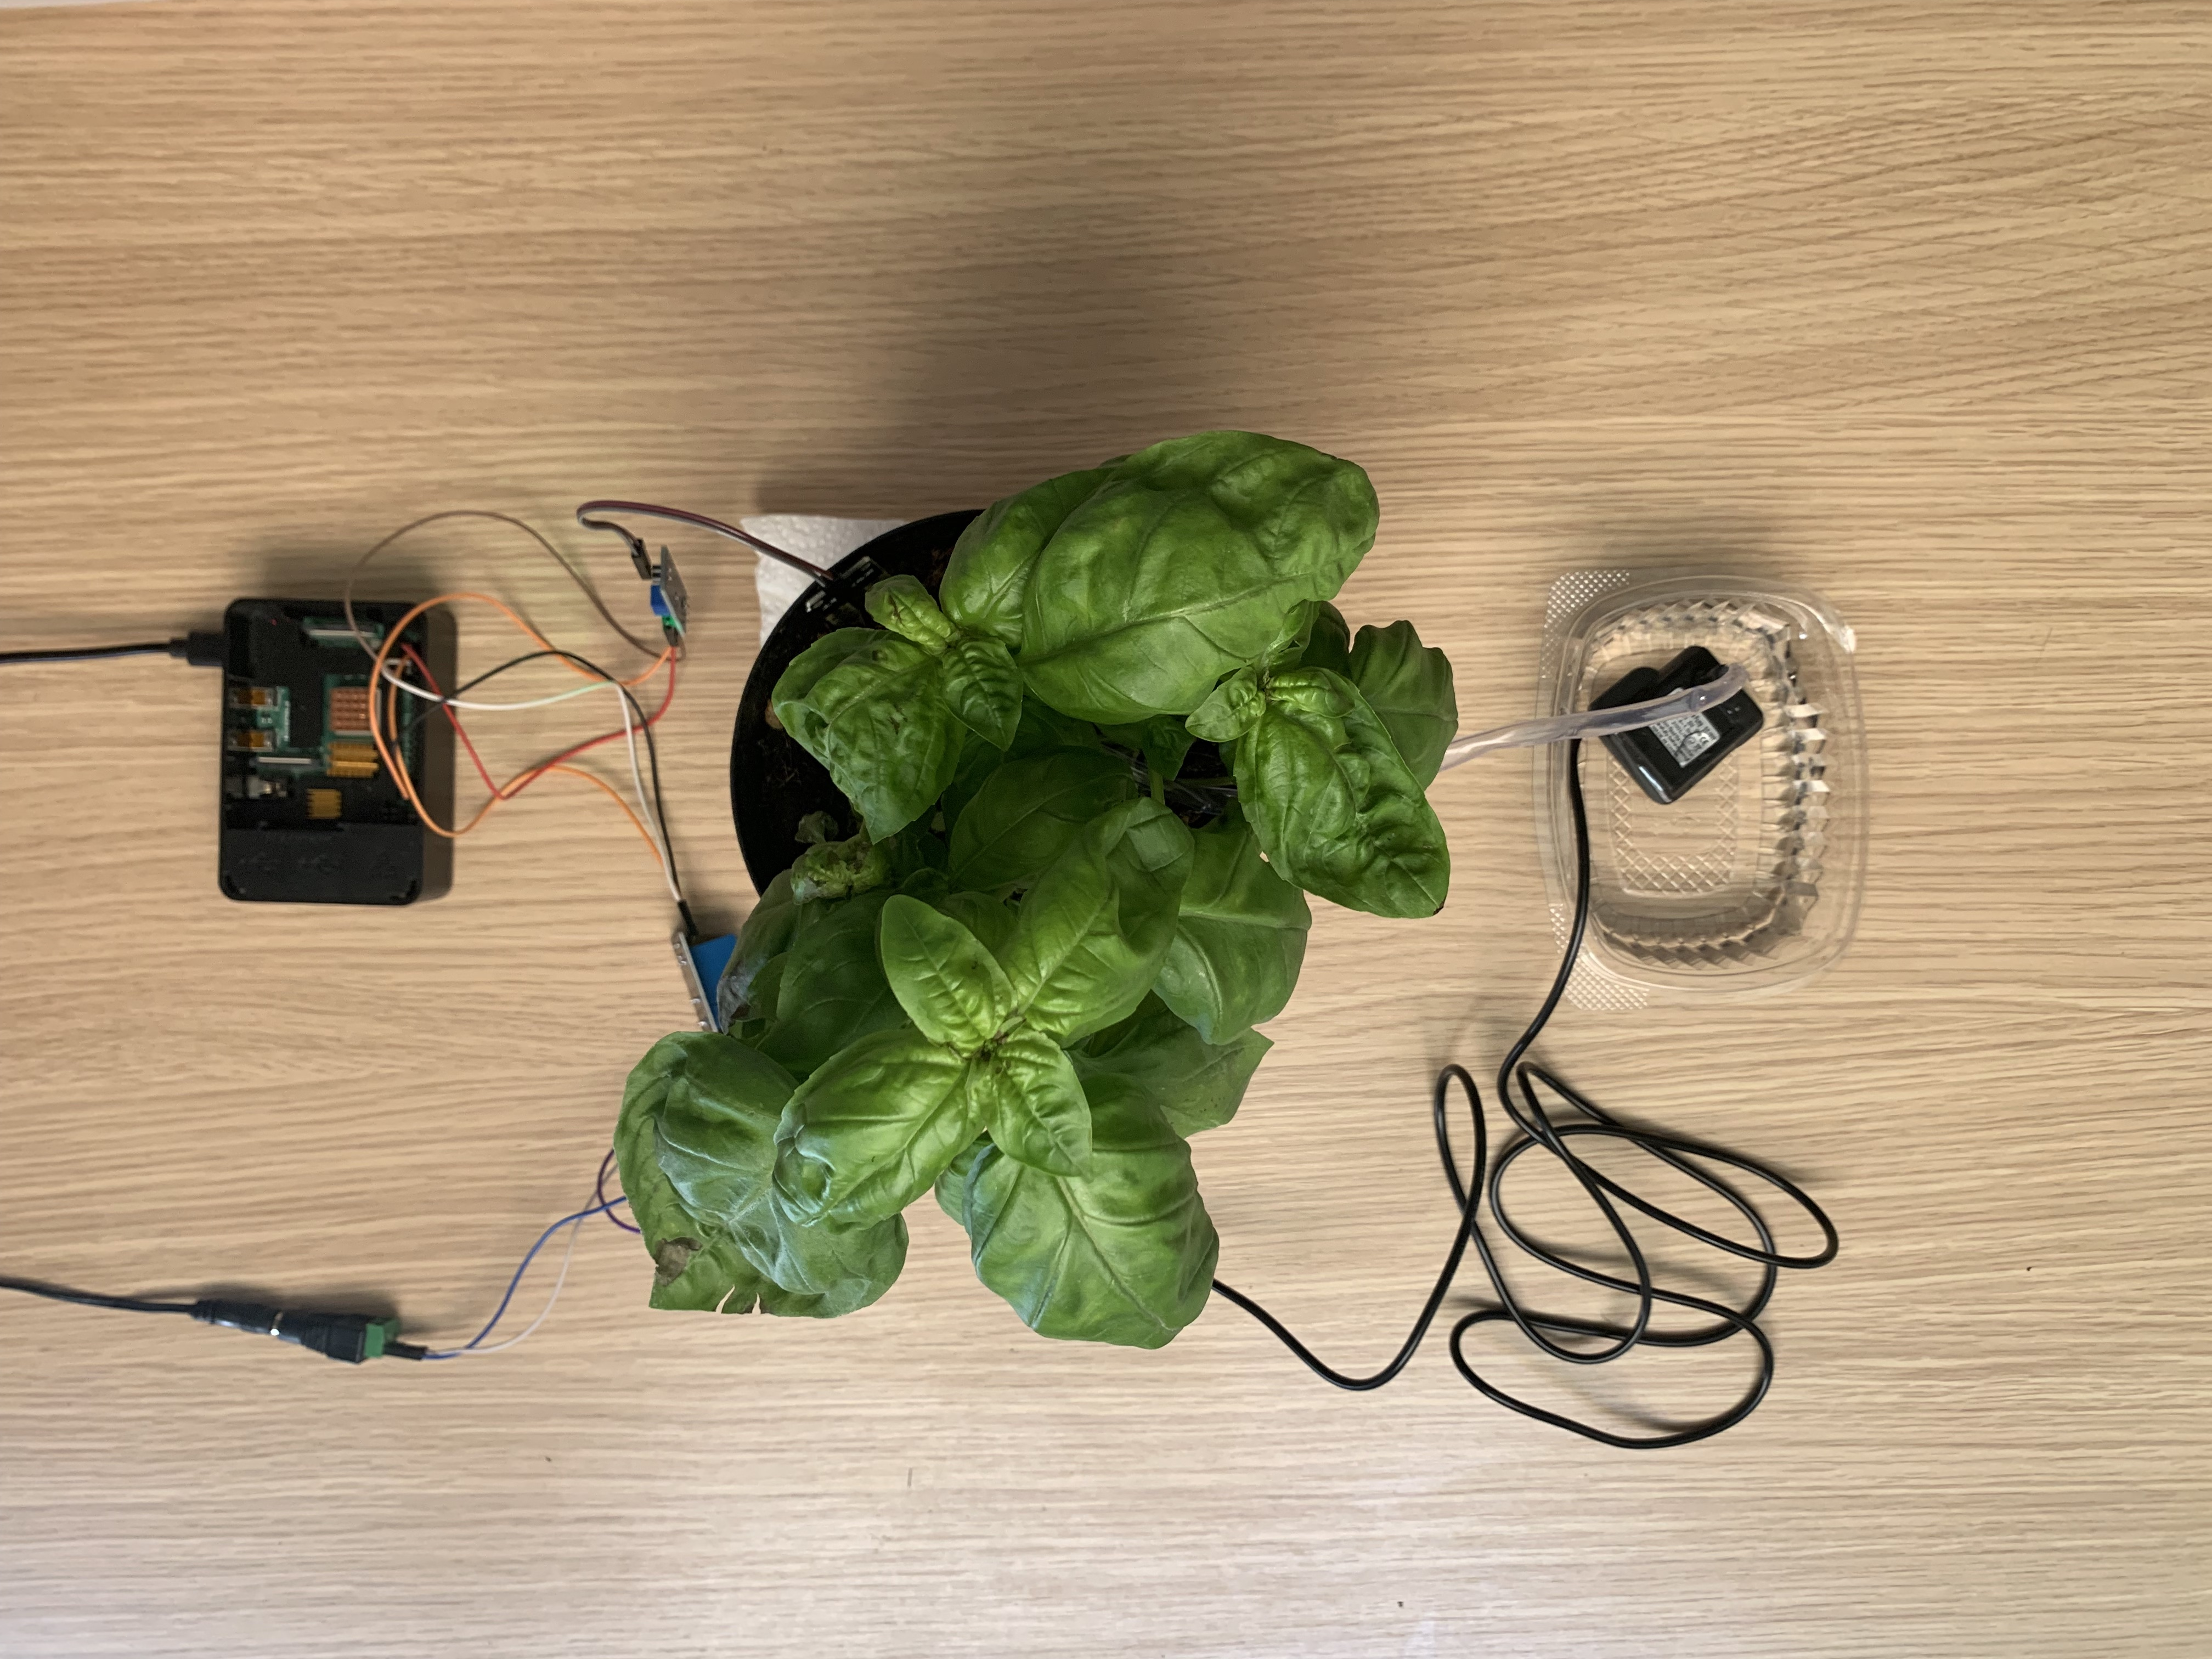
\includegraphics[width=12cm]{Immagini/smart_garden_4}
    \caption{Smart Garden dall'alto}
    \label{fig:smart_garden_4}
\end{figure}

\appendix
%\input{schema_elettrico}
%\input{Appendix1}
%\input{Appendix2}

\printbibliography

\printindex

\chapter*{Ringraziamenti}
Il mio ringraziamento va al professor Michele Loreti per avermi sostenuto e guidato durante la tesi ed il percorso di formazione universitario e a Ivan Compagnucci, studente Unicam della Magistrale che mi ha aiutato a sviluppare il sistema IOT partendo da una base gi\'a sviluppata precedentemente da lui in arduino. 

\end{document}